\documentclass[a4paper, 11pt]{article}
\pdfoutput=1 % if your are submitting a pdflatex (i.e. if you have
             % images in pdf, png or jpg format)

\usepackage{jcappub} % for details on the use of the package, please
                     % see the JCAP-author-manual

\usepackage[T1]{fontenc} % if needed

\usepackage{array}
\usepackage{enumitem}
\usepackage{graphicx}
\usepackage{epstopdf, epsfig}
\usepackage{subcaption}
\usepackage{tikz}
\usetikzlibrary{intersections}
\usepackage{pgfplots}
\usepackage{ environ}
\usepackage{framed}
\usepackage{bm}
\usepackage[us,12hr]{datetime}
\usepackage{algorithmic}
\usepackage[ruled]{algorithm2e}

\title{The statistical properties of the two-dimensional caustic skeleton}

\author[a,b]{Job Feldbrugge}
\author[c]{Rien van de Weygaert}

\affiliation[a]{Perimeter Institute for Theoretical Physics, University of Waterloo, Waterloo, Canada}
\affiliation[b]{Physics department, Carnegie Mellon University, Pittsburgh, United States}
\affiliation[c]{Kapteyn Astronomical Institute, University of Groningen, Groningen, The Netherlands}

\emailAdd{jfeldbrugge@perimeterinstitute.ca}

\newcommand{\aap}{Astron. Astrophys.}
\newcommand{\mnras}{Mon. Not. R. Astron. Soc.}
\newcommand{\apj}{Astrophys. J.}
\newcommand{\jcap}{Journal of Cosmology and Astroparticle Physics}
\newcommand{\nat}{Nature}
\newcommand{\apjs}{Astrophysical Journal, Supplement}
\newcommand{\apjl}{Astrophysical Journal, Letters}
\newcommand{\aj}{Astronomical Journal}
\newcommand{\prd}{Physical Review D}

\newcommand{\Remark}[1]      {{\small {\textcolor{red}{  \sf{[[{#1}]]}}}}} 

\newtheorem{thr}{Theorem:}
\newtheorem{lemma}{Lemma}
\newtheorem{corollary}{Corollary}

\abstract{
To Do list:
\begin{itemize}
\item Evolve the constrained initial conditions in time.
\end{itemize}

\noindent Last compiled on: {\color{red} \currenttime\ at \today}}

\graphicspath{
{./figures/}}

\begin{document}
%\pagecolor{yellow!30!orange}
\maketitle

%%%%%%%%%%%%%%%%%%%%%%%%%%%%%%%%%%%%%%%%%%%%%%%%%%%%%%%%%%%%%%%%
\section{Introduction}
The large-scale structures of our Universe are routinely observed through the distribution of galaxies, neutral gas, or dark matter. Upcoming cosmological redshift surveys will map the cosmic web in even greater detail, revealing a lot of information about the geometry of the large-scale structure, the properties of the galaxies embedded in the cosmic web, and fundamental physics. The cosmic web is not only observable through the distribution of galaxies, but, in fact, directly influences their formation processes. For example, cosmic streams following the filamentary structure of the cosmic web significantly affect the angular momentum and spin alignment of galaxies. To exploit the full information in the next generation of cosmological surveys, it is increasingly important to develop an analytic framework that models the mildly non-linear evolution of the different features of the cosmic web -- the voids, the walls, the filaments and the clusters -- and their influence on the embedded halos and galaxies. Building on work by Arnol'd, Zel'dovich and collaborators, we recently solved a long-standing problem in Lagrangian catastrophe theory, enabling us to build such a framework based on the evolution of dark matter sheet in six-dimensional \textit{phase-space} and the corresponding \textit{caustic skeleton}. In this paper, we study the statistical properties of the caustic skeleton in the two-dimensional context to highlight the different features of the caustic skeleton. The calculations can straightforwardly be extended to the three-dimensional cosmic web, following in a future publication. Note that while the results presented here form a toy-model for the three-dimensional cosmic web, the analysis has direct implications to the caustic networks emerging from strong lensing by a thin random lens screen in ray optics.

In the standard scenario of structure formation, both galaxies and the cosmic web form through the gravitational collapse of primordial density perturbations present at the epoch of recombination. These perturbations take the form of a statistically homogeneous and isotropic random process with properties inherited from the quantum physics of the early universe. In this paper, we will generally assume the primordial density field to be a realization of a Gaussian random field\footnote{The analysis can be extended to include primordial non-Gaussianities.}. As was realized early on, the stochastic properties of the initial conditions place large scale structure formation in close correspondence with the path integral methods employed in statistical and quantum field theory. In both theories, observables are expressed as expectation values, which can be evaluated by inserting them into the path integral. This has led to numerous application of Feynman rules to large scale structure formation. In particular, in the last decade, significant progress has been made on the modelling of the power spectrum and the bi-spectrum of the late time universe in the effective field theory program, pushing the predictions to increasingly smaller scales. However, notwithstanding their success, it should be stressed that the power- and bi-spectra are not necessarily sensitive probes for the geometric information encoded in the phase-correlations of the cosmic web. Though powerful, these approaches do not capture the full information of the observed non-linear structure. 

A significant effort has been made to relate the geometry of the cosmic web to the initial conditions, by associating the clusters, filaments, walls, and voids to the maxima, saddle points, and minima of the primordial density perturbation. This proposal is based on the mathematical Morse-Smale complex. However, the association of the different element of the cosmic web with the critical points of the density perturbation has no rigorous underpinning and is unable to predict the geometric properties of the late time cosmic web. In this paper, we will demonstrate that the caustic skeleton yields a more refined definition of the geometric properties of the late time cosmic web in the initial conditions through the recently derived \textit{caustic conditions} in Lagrangian fluid dynamics. These conditions are directly related to the phase-space evolution of the dark matter sheet. We study the statistical properties of the caustics in the Zel'dovich approximation of large-scale structure formation and evolve the skeleton to the present using the \textit{scotch flow}, truncating the Zel'dovich flow. In the future, this flow can be refined to include more advanced analytical approximations such as second-order Lagrangian perturbation theory (2LPT) or the recently developed effective field theory schemes. We provide a detailed comparison between this caustic skeleton and the Morse-Smale skeleton.

Besides the perturbative Feynman methods from quantum physics, the study of the cosmic web has seen the application of numerical lattice methods. In particular, noteworthy is constrained Gaussian random field theory, constructing realizations of Gaussian random fields subject to a set of constraints. Using these techniques, we can construct realizations of random fields with peaks, saddle points, and valleys at specified locations. These realizations can subsequently be studied with $N$-body simulations. This effort has recently led to the reconstruction of realistic initial conditions corresponding to cosmological surveys of our local Universe. In this paper, we will show that the same methods can be applied to the caustic skeleton, revealing the statistical properties of patches that form the walls, filaments and clusters of the cosmic web. A fine-grained and detailed description of the characteristic formation histories of walls, filaments, and clusters is a valuable step towards a first principle understanding of the interplay between the cosmic web and galaxy formation.

\begin{framed}
{\color{red}Summary of sections.}
\end{framed}

%%%%%%%%%%%%%%%%%%%%%%%%%%%%%%%%%%%%%%%%%%%%%%%%%%%%%%%%%%%%%%%%
\section{Lagrangian fluid dynamics and the caustic skeleton}
Lagrangian fluid dynamics is well-known to be an effective tool to model the cosmic web, exemplified by the famous Zel'dovich approximation, second-order Lagrangian perturbation theory ($2$LPT), and $N$-body simulations. The Lagrangian fluid consists of a collection of mass elements, evolving according to the Lagrangian map, $\bm{x}_t:\mathcal{L}\to \mathcal{E}$,
\begin{align}
\bm{x}_t(\bm{q}) \equiv \bm{q} + \bm{s}_t(\bm{q})\,,
\end{align}
with the displacement field $\bm{s}_t$, describing the motion of the mass elements, from the initial position $\bm{q}$ in Lagrangian space $\mathcal{L}$ to the position $\bm{x}_t(\bm{q})$ at time $t$ in Eulerian space $\mathcal{E}$. A $d$-dimensional fluid forms a $d$-dimensional manifold in $2d$-dimensional \textit{phase-space}. In this paper, we define phase-space as the product of the initial (Lagrangian) and final (Eulerian) position of the mass elements\footnote{This definition of phase-space is related to the more common definition in terms of the position and the momentum of particles.}. This dark matter sheet in phase-space, defined by the set $\{(\bm{q},\bm{x}') \in \mathcal{L}\times \mathcal{E}\, |\, \bm{x}_t(\bm{q})=\bm{x}'\}$ at time $t$, starts simple, \textit{i.e.}, $\bm{x}_0(\bm{q})=\bm{q}$, but can develop intricate geometries at later times. After shell-crossing, the manifold can in particular form multi-stream regions where multiple $\bm{q}$'s map to the same point in Eulerian space. The boundaries between regions with a different number of streams are known as caustics. These caustics are important features of the Lagrangian fluid, as they mark a qualitative change in the geometry and lead to a spike in the density field which accumulate mass from their environments. In this paper, we study the statistical properties of the caustics in large-scale structure formation to analyse the geometry of the cosmic web.

The Lagrangian map $\bm{x}_t$ can deform the shape of a mass element, but will always preserves its mass. As a consequence, the density of the Lagrangian fluid is determined by the Jacobian of the Lagrangian map, \textit{i.e.},
\begin{align}
\rho_t(\bm{x}) &= \sum_{\bm{q} \in A_t(\bm{x})} \frac{\bar{\rho}}{|\det \nabla_{\bm{q}} \bm{x}_t|}\nonumber \\
&= \sum_{\bm{q} \in A_t(\bm{x})} \frac{\bar{\rho}}{|\det (I + \nabla_{\bm{q}} \bm{s}_t)|}\,,
\label{eq:LagrangianDensity}
\end{align}
with $\bar{\rho}$ the mean initial density, and the pre-image
\begin{align}
A_t(\bm{x}') \equiv \bm{x}_t^{-1}(\bm{x}') = \{\bm{q} \,|\, \bm{x}_t(\bm{q})= \bm{x}'\}\,,
\end{align}
consisting of the the points in Lagrangian space, $\mathcal{L}$, that reach $\bm{x}'\in \mathcal{E}$ in time $t$. The set $A_t(\bm{x}')$ generally consists of an odd number of points, counting the number of streams in a given region. The density spikes at the caustics, when the Jacobian vanishes, \textit{i.e.}, $\det \nabla_{\bm{q}}\bm{x}_t=0$, separating two regions with a different number of streams. 

In large scale structure formation, the Lagrangian map $\bm{x}_t$ is determined by the conservation of mass, the Euler equation, and the Poisson equation. In comoving coordinates, the Euler and the Poisson equations take the form
\begin{align}
\frac{\mathrm{d} \bm{v}_t(\bm{q})}{\mathrm{d}t} + \frac{\dot{a}(t)}{a(t)}\bm{v}_t(\bm{q}) &= - \frac{1}{a(t)} \nabla_{\bm{q}} \phi_t(\bm{q})\,,\\
\nabla_{\bm{q}}^2 \phi_t(\bm{q}) &= 4 \pi G a^2(t) \rho_u(t) \delta_t(\bm{q})\,,
\end{align}
with the velocity
\begin{align}
\bm{v}_t = a(t) \frac{\mathrm{d}\bm{s}_t}{\mathrm{d}t}\,,
\end{align}
the scale factor $a$ satisfying the Friedmann-Lema\^itre equation (normalized to unity for the present epoch $a(t_0)=1$ with $t_0$ the age of the universe), the gravitational potential $\phi_t$, Newton's constant $G$, the uniform cosmic density $\rho_u$, and the density perturbation
\begin{align}
\delta_t(\bm{q}) = \frac{\rho_t(\bm{q})}{\bar{\rho}} -1\,.
\end{align}
The conservation of mass establishes a relation between the density perturbation $\delta_t$ and the displacement field $\bm{s}_t$ through the Lagrangian density \eqref{eq:LagrangianDensity}.

%%%%%%%%%%%%%%%%%%%%%%%%%%%%%%%%%%%%%%%%%%%%%%%%%%%%%%%%%%%%%%%%
\subsection{The Zel'dovich approximation}
The Zel'dovich approximation is the first order approximation in Lagrangian fluid dynamics, for which the displacement field factorizes into a spatial and a temporal part
\begin{align}
\bm{s}_t(\bm{q}) = - b_+(t) \nabla_{\bm{q}} \Psi(\bm{q})\,.
\end{align}
The growing mode $b_+$ is a natural time parameter satisfying the differential equation
\begin{align}
\frac{\mathrm{d}^2 b_+(t)}{\mathrm{d}t^2} + 2 \frac{\dot{a}(t)}{a(t)} \frac{\mathrm{d} b_+(t)}{\mathrm{d}t} = 4 \pi G \rho_u(t) b_+(t)\,.
\end{align}
The displacement potential $\Psi$ captures the geometry, and is proportional to the primordial gravitational potential
\begin{align}
\Psi(\bm{q}) &=\frac{1}{4 \pi G a^2 \rho_0}\phi_0(\bm{q})%\\
%&= \frac{2}{3\Omega_0 H_0^2}\phi_0(\bm{q})
\,,
\end{align}
expressed in terms of the current total energy density %$\Omega_0$ and
$\rho_0$,
%the current Hubble parameter $H_0$,
and the linearly extrapolated gravitational potential $\phi_0$. Note that the Poisson equation relates the primordial gravitational potential to the primordial density perturbation
\begin{align}
\nabla ^2 \phi &= 4 \pi G a^2 \rho_u \delta\,,%\\
%&= \frac{3}{2} \Omega H^2 a^2 \delta\,,
\end{align}
where we dropped the subscript. In the Zel'dovich approximation, the mass elements follow linear trajectories that are completely determined by the primordial gravitational potential. The approximation accurately describes single-stream regions but fails when mass streams overlap and gravitational interactions between mass elements become important.

The density for the two-dimensional Zel'dovich approximation takes the form
\begin{align}
\rho(\bm{x}) = \sum_{\bm{q} \in A_t(\bm{x})}\frac{\bar{\rho}}{|1-b_+(t)\lambda_1(\bm{q})||1-b_+(t)\lambda_2(\bm{q})|}\,,
\end{align}
with the eigenvalue fields $\lambda_i$ (assuming the ordering $\lambda_1(\bm{q}) \geq \lambda_2(\bm{q})$) of the deformation tensor
\begin{align}
\bm{\psi} =
\begin{pmatrix}
T_{11} & T_{12}\\
T_{12} & T_{22}
\end{pmatrix}\,,
\end{align}
with the derivatives of the displacement potential $T_{i j \dots k} = \frac{\partial}{\partial q_i}\frac{\partial}{\partial q_j}\dots \frac{\partial}{\partial q_k} \Psi$. The eigenvalue and eigenvector fields are defined by
\begin{align}
\bm{\psi}(\bm{q}) \bm{v}_i(\bm{q}) =\lambda_i(\bm{q}) \bm{v}_i(\bm{q})\,,
\end{align}
yielding the non-linear identities
\begin{align}
\lambda_{1,2} &= \frac{T_{11}+T_{22} \pm \sqrt{4T_{12}^2 + (T_{11}-T_{22})^2}}{2}\,,\\
\bm{v}_{1,2} &\propto \left(T_{11}-T_{22} \pm \sqrt{4T_{12}^2 + (T_{11}-T_{22})^2}\,,\,2 T_{12}\right)\,,
\end{align}
with the plus and the minus sign corresponding to the subscript $1$ and $2$. Note that in the eigenframe of the deformation tensor, \textit{i.e.}, $T_{12}=0$, the eigenvalue and eigenvector fields simplify to
\begin{align}
\lambda_1&=T_{11}\,, \quad \bm{v}_1=(1,0)\,,\\
\lambda_{2}&=T_{22}\,, \quad \bm{v}_2=(0,1)\,,
\end{align}
assuming without loss of generality $T_{11}\geq T_{22}$.
\begin{figure}
\centering
\begin{subfigure}[b]{0.49\textwidth}
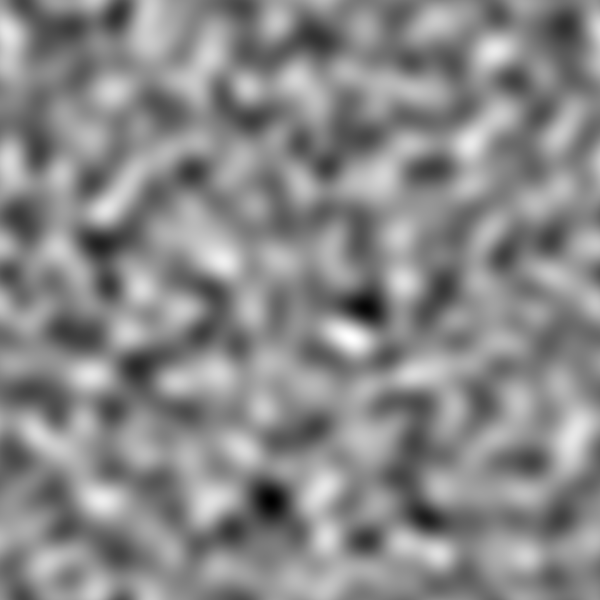
\includegraphics[width=\textwidth]{delta}
\caption{The density perturbation $\delta$}
\label{fig:delta}
\end{subfigure}
\begin{subfigure}[b]{0.49\textwidth}
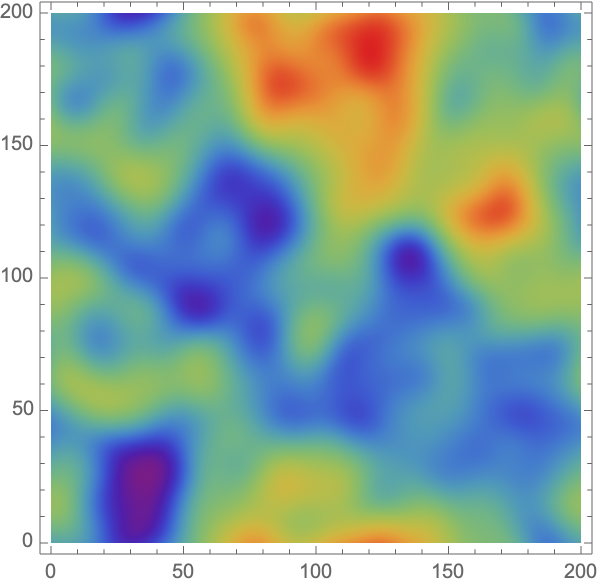
\includegraphics[width=\textwidth]{Psi}
\caption{The displacement potential $\Psi$}
\label{fig:Psi}
\end{subfigure}\\
\begin{subfigure}[b]{0.49\textwidth}
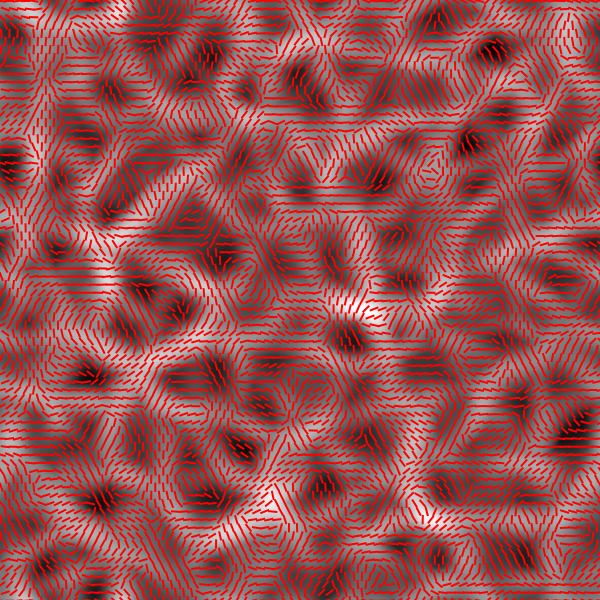
\includegraphics[width=\textwidth]{a}
\caption{The first eigenvalue and eigenvector fields $\lambda_1$, and $\bm{v}_1$}
\label{fig:lambda1}
\end{subfigure}
\begin{subfigure}[b]{0.49\textwidth}
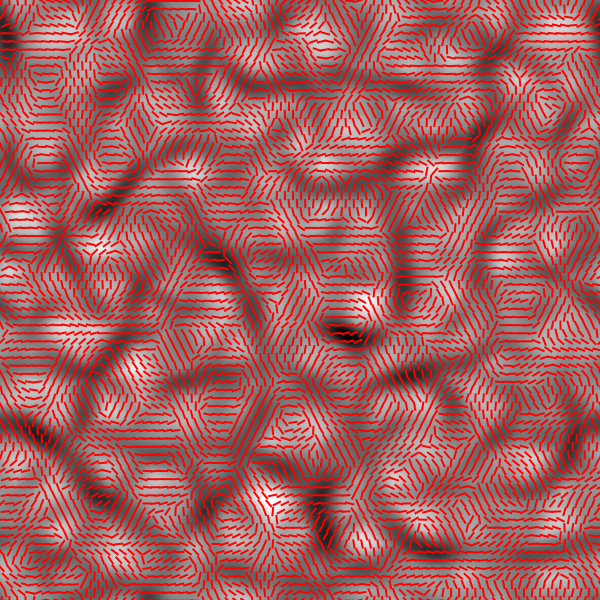
\includegraphics[width=\textwidth]{b}
\caption{The second eigenvalue and eigenvector fields $\lambda_2$, and $\bm{v}_2$}
\label{fig:lambda2}
\end{subfigure}
\caption{The initial density perturbation $\delta$, the corresponding displacement potential $\Psi$, and the eigenvalue and the eigenvector fields in a periodic $10\text{ Mpc } \times 10 \text{ Mpc}$ box with $2048 \times 2048$ grid points. The density perturbation, the displacement potential and the eigenvalue fields are displaced using different grey tones. The eigenvector fields are represented by the red lines. For this example we use the hierarchical power-law $k^{-2}$ smoothed with a Gaussian filter at scale $R=0.25 \text{ Mpc}$, \textit{i.e.}, $P_{\Psi}(k) \propto k^{-2}e^{-R^2 k^2}$.}
\label{fig:Example}
\end{figure}

By studying the geometry and topology of the deformation tensor $\bm{\psi}$, we can anticipate the structure of the cosmic web. Given the initial density perturbation $\delta$ (see figure \ref{fig:delta}) and the corresponding displacement potential $\Psi$ (see figure \ref{fig:Psi}) we evaluate the eigenvalue and eigenvector fields $\lambda_i$ and $\bm{v}_i$ of the deformation tensor $\bm{\psi}$ (figures \ref{fig:lambda1} and \ref{fig:lambda2}). Observe that while the density perturbation and the displacement potential consist of blob-like structures, the eigenvalue fields are non-Gaussian and include fibre-like structures representing the filaments and the clusters at their intersections.

%%%%%%%%%%%%%%%%%%%%%%%%%%%%%%%%%%%%%%%%%%%%%%%%%%%%%%%%%%%%%%%%
\subsection{Geometric optics}
Before describing the caustics of the Lagrangian map, we discuss a close parallel of the Zel'dovich approximation with optical systems in the ray optics. The Kichhoff-Fresnel integral for lensing of monochromatic radiation by a thin lens-plane $L$,
\begin{align}
\psi_{KF}(\bm{y}) =\mathcal{N} \int_L e^{i \nu T(\bm{x},\bm{y})}\mathrm{d}\bm{x}\,,
\end{align}
captures the the full wave nature of light as an oscillatory integral over the lens-plane, with the frequency of the radiation $\nu$, the time-delay 
\begin{align}
T(\bm{x},\bm{y}) =\frac{d_l d_s}{d_{ls}}\left( \frac{(\bm{x}-\bm{y})^2}{2} + \frac{d_{ls}}{d_ld_s}\varphi(\bm{x})\right)\,,
\end{align}
the distance between the observer and the lens-plane $d_l$, the distance between the observer and the source $d_s$, and the distance between the lens-plane and the source $d_{ls}$. The first term in the time-delay function captures the geometry of a ray passing from the source to the point on the lens-plane $\bm{x}$, to the point on the screen $\bm{y}$. The second term describes the phase variation $\varphi$ received while passing through the lens. The normalization factor $\mathcal{N} = \frac{\nu}{2 \pi i} \frac{d_l d_s}{d_{ls}}$, normalizes the intensity of the diffraction pattern $I_{KF}(\bm{y}) = |\psi_{KF}(\bm{y})|^2$ to unity in the absence of a lens, \textit{i.e.}, $I_{KF}(\bm{y})=1$ when $\varphi(\bm{x})=0$.



For high frequencies, the critical points dominate the integral. In accordance with Fermat's principle, the classical rays correspond to stationary points of the time-delay function
\begin{align}
0 &= \nabla_{\bm{x}} T(\bm{x},\bm{y})\nonumber\\
&= \bm{x} - \bm{y} + \frac{d_{ls}}{d_ld_s} \nabla \varphi(\bm{x})\,,
\end{align}
inducing the Lagrangian map
\begin{align}
\bm{\xi}(\bm{x}) = \bm{x} + \frac{d_{ls}}{d_ld_s} \nabla \varphi(\bm{x})\,.
\end{align}
A ray passing from the source to the point $\bm{x}$ on the lens $L$ intersects the screen at $\bm{\xi}(\bm{x})$. Note that the Lagrangian map $\bm{\xi}$ is independent of the frequency of the radiation. The Lagrangian map resembles the definition of the Zel'dovich approximation with the growing mode $b_+ \equiv -d_{ls}/(d_l d_s)$ and the displacement potential $\Psi \equiv \varphi$. The intensity in the geometric approximation, following from the saddle point approximation of the Kirchhoff-Frensel integral,
\begin{align}
I_{KF}(\bm{y})
&= \sum_{\bm{x} \in \bm{\xi}^{-1}(\bm{y})} \frac{1}{|\det \nabla \bm{\xi}(\bm{x})|} \nonumber\\
&=\sum_{\bm{x} \in \bm{\xi}^{-1}(\bm{y})} \frac{1}{|1+\lambda_1(\bm{x})||1+\lambda_2(\bm{x})|} \,,
\end{align}
is analogous to the density for a Lagrangian fluid, with the eigenvalue fields $\lambda_i$ of the deformation tensor,
\begin{align}
\frac{d_{ls}}{d_ld_s} \mathcal{H} \varphi(\bm{x}) \bm{v}_i(\bm{x}) = \lambda_i(\bm{x}) \bm{v}_i(\bm{x})\,,
\end{align}
with the Hessian operator $\mathcal{H}$. The intensity pattern in the geometric optics is mathematically equivalent to the density field in the Zel'dovich approximation. Consequently, the study of caustics arising in two-dimensional large scale structure formation can directly be used to understand the geometry of the caustics formed by strong lensing by a turbulent medium. Consider for example lensing by the interstellar medium or waves in a swimming pool.

%%%%%%%%%%%%%%%%%%%%%%%%%%%%%%%%%%%%%%%%%%%%%%%%%%%%%%%%%%%%%%%%
\subsection{The caustic skeleton}
The caustics in a Lagrangian fluid can arise in a number of morphologies classified by Lagrangian catastrophe theory (see table \ref{table:caustics} for an overview). In a recent paper, we showed that these morphologies are completely determined by the eigenvalue and eigenvector fields of the deformation tensor. We here summarize the various caustics arising in the two-dimensional large scale structure.

\begin{table}
\centering
{\scriptsize
\begin{tabular}{ |l | l | l | l | l|}
\hline
Symbol & Name & 2D cosmic web & 3D cosmic web & Caustic conditions\\
\hline
$A_2$ & fold & shall-crossing & shell-crossing & $\lambda_i = 1/ b_+$ \\
\hline
$A_3$ & cusp & filament & wall & $\lambda_i > 1/ b_+$, and $\lambda_{i,i} = 0$\\
\hline
$A_4$ & swallowtail & cluster & filament & $\lambda_i > 1/ b_+$, $\lambda_{i,i} = 0$, and $\lambda_{i,ii} = 0$\\
\hline
$D_4^{\pm}$ & elliptic/hyperbolic & cluster & filament & $\lambda_1 > 1/ b_+$, and $\lambda_1 = \lambda_2$\\
\hline
$A_5$ & butterfly & N.A. & cluster & $\lambda_i > 1/ b_+$, $\lambda_{i,i} = 0$, $\lambda_{i,ii} = 0$, and $\lambda_{i,iii} = 0$\\
\hline
$D_5$ & parabolic & N.A. & cluster & $\lambda_1 > 1/ b_+$, $\lambda_1 = \lambda_2$, and $\lambda_{1,11}=0$\\
\hline
\end{tabular}
}
\caption{Elements of the caustic skeleton, with the directional derivatives of the eigenvalue fields $\lambda_{i,j} \equiv \bm{v}_j \cdot \lambda_i$, $\lambda_{i,jk} \equiv \bm{v}_k \cdot \nabla \lambda_{i,j}$, and $\lambda_{i,jkl} \equiv \bm{v}_l \cdot \nabla \lambda_{i,jk}$ .}
\label{table:caustics}
\end{table}

%%%%%%%%%%%%%%%%%%%%%%%%%%%%%%%%%%%%%%%%%%%%%%%%%%%%%%%%%%%%%%%%
\subsubsection{Shell-crossing}
The density spikes during the phenomenon of shell-crossing, where different matter stream start to cross and Jacobian vanishes. Shell-crossing is the simplest catastrophe corresponding to the fold caustic $A_2$. At a given time $t$, shell-crossing takes place on the manifold
\begin{align}
A_2^i(t) = \{\bm{q}\,|\, 1- b_+(t)\lambda_i(\bm{q})=0\}\,,
\end{align}
for $i=1,2$. The fold manifold is an iso-contour of the eigenvalue field, indicating that the caustics follow the geometry of the eigenvalue field rather than the density perturbation (see the grey curves in figures \ref{fig:eigen1_1} and \ref{fig:eigen1_2}). In the Zel'dovich approximation, these fold curves bound different multi-stream regions (see the grey curves in figures \ref{fig:Zeldovich_1} and \ref{fig:Zeldovich_2}). After shell-crossing, the Zel'dovich approximation fails to capture the evolution of the mass elements. However, the fold curve in Lagrangian space is still a good marker for the mass elements that undergo shell-crossing at a given time (see figure grey curves in figures \ref{fig:Nbody_1} and \ref{fig:Nbody_2}). The region that has already shell-crossed, forming a multi-stream structure, is given by the big caustic
\begin{align}
A_2^i = \cup_{0 \leq t \leq t_0} A_2^i(t)\,,
\end{align}
with the current time $t_0$ (the regions enclosed by the grey curves in figure \ref{fig:eigen1_1} and \ref{fig:eigen1_2}). Note that the Zel'dovich approximation in figures \ref{fig:Zeldovich_1} and \ref{fig:Zeldovich_2} is an exact description of the lensing by a random screen in geometric optics.

%%%%%%%%%%%%%%%%%%%%%%%%%%%%%%%%%%%%%%%%%%%%%%%%%%%%%%%%%%%%%%%%
\subsubsection{Filaments}
The filaments in the two-dimensional cosmic web correspond to the cusp caustic $A_3$. Cusp caustics forms when the shell-crossing region $A_2^i(t)$ is mapped to a non-differential point. The cusp manifold is defined in terms of both the eigenvalue and the eigenvector fields
\begin{align}
A_3^i(t)=\{\bm{q}\,|\,1- b_+(t)\lambda_i(\bm{q})=0 \text{ and } \bm{v}_i \cdot \nabla \lambda_i(\bm{q}) = 0\}\,,
\end{align}
defining points in space. These cusp points can be observed as the intersection between the grey and red curves in the two lower rows of figure \ref{fig:visualization}. Over time, these points trace out the big cusp caustic
\begin{align}
A_3^i = \cup_{0 \leq t \leq t_0} A_3^i(t)\,,
\end{align}
corresponding to the filaments of the two-dimensional cosmic web (see the red curves in the two lower rows of figure \ref{fig:visualization}).

These cusp curves change topology at the Morse points
\begin{align}
A_3^{i+} = \{\bm{q}\,|\,\bm{q} \text{ is a maximum of } \lambda_i(\bm{q})|_{A_3^i}\}\,,
\end{align}
corresponding to the creation of a filament and
\begin{align}
A_3^{i-} = \{\bm{q}\,|\,\bm{q} \text{ is a minimum of } \lambda_i(\bm{q})|_{A_3^i}\}\,,
\end{align}
corresponding to the merger of two filaments. In these definitions, the expression $\lambda_i|_C$ indicates the restriction of the eigenvalue field $\lambda_i$ to the manifold $C$ (see the black points in the two lower rows of figure \ref{fig:visualization}). Note that the cusp curve $A_3^i$ passes through all the critical points of the eigenvalue field for which $\lambda_i \geq 1/b_+(t_0)$, since $\nabla \lambda_i=0$ implies $\bm{v}_i \cdot \nabla \lambda_i=0$. Further note that such a critical point will always correspond to a Morse point $A_3^{i\pm}$ since $\lambda_i|_{A_3^i}$ is a maximum or minimum in the critical point. However, the reverse is not true, \textit{i.e.}, a point $\bm{q} \in A_3^i$ can be a local extrema of $\lambda_i|_{A_3^i}$ while it is not a critical point of $\lambda_i$. In this case, the Morse point arises due to the geometry of the cusp curve. This can be observed when comparing the critical points of the first eigenvalue field in figure \ref{fig:eigen1_MS} with the black Morse points in figures \ref{fig:eigen1_1} and \ref{fig:eigen1_2}.

%%%%%%%%%%%%%%%%%%%%%%%%%%%%%%%%%%%%%%%%%%%%%%%%%%%%%%%%%%%%%%%%
\subsubsection{Clusters}
According to catastrophe theory, the two-dimensional cosmic web can form two types of clusters. The first, known as the swallowtail caustic $A_4$, forms when the big cusp curve forms a non-differentiable point under the Lagrangian map. These points satisfy the three conditions
\begin{align}
A_4^i(t)=\{\bm{q}\,|\,
1- b_+(t)\lambda_i(\bm{q})=0,\,
 \bm{v}_i \cdot \nabla \lambda_i(\bm{q}) = 0,\,
 \bm{v}_i \cdot \nabla(\bm{v}_i \cdot \nabla \lambda_i(\bm{q})) = 0\}\,,
\end{align}
defining points in space-time. The swallowtails trace the big caustic
\begin{align}
A_4^i = \cup_{0 \leq t \leq t_0} A_4^i(t)\,,
\end{align}
corresponding to the clusters of the two-dimensional cosmic web (see the blue points in the two lower rows of figure \ref{fig:visualization}). The swallowtail points are relatively numerous and form during the gravitational collapse along a single direction.

The second rarer and more dense cluster type is associated to the umbilic caustic $D_4^{\pm}$ where the two eigenvalue fields coincide,
\begin{align}
D_4^{12 \pm}(t) = \{\bm{q}\,|\,1 - b_+(t)\lambda_1(\bm{q}) = 1 - b_+(t) \lambda_2(\bm{q}) = 0\}\,,
\end{align}
defining points in space-time. These clusters form due to gravitational collapse along two directions. The umbilic caustic forms in two morphologies. The elliptic and the hyperbolic form distinguished by the sign of the determinant $ \mathcal{S}_{\mathcal{M}}$,
\begin{align}
\mathcal{S}_{\mathcal{M}} &= \frac{1}{2}((\lambda_i - \lambda_j)_{,j} \lambda_{i,j} - (\lambda_i - \lambda_j)_{,i} \lambda_{j,i}\nonumber\\
& = \frac{1}{2} [(T_{112}-T_{222})T_{112} - (T_{111}-T_{122})T_{122}]\,.
\end{align}
Over time, these points trace the big umbilic caustic
\begin{align}
D_4^{12 \pm} = \cup_{0 \leq t \leq t_0} D_4^{12 \pm}(t)\,.
\end{align}
See the yellow points in the two lower rows of figure \ref{fig:visualization}. The collection of these caustics form the two-dimensional caustic skeleton. In the three-dimensional case the situation is slightly more involved (see table \ref{table:caustics}).

\begin{figure}
\centering
\begin{subfigure}[b]{0.32\textwidth}
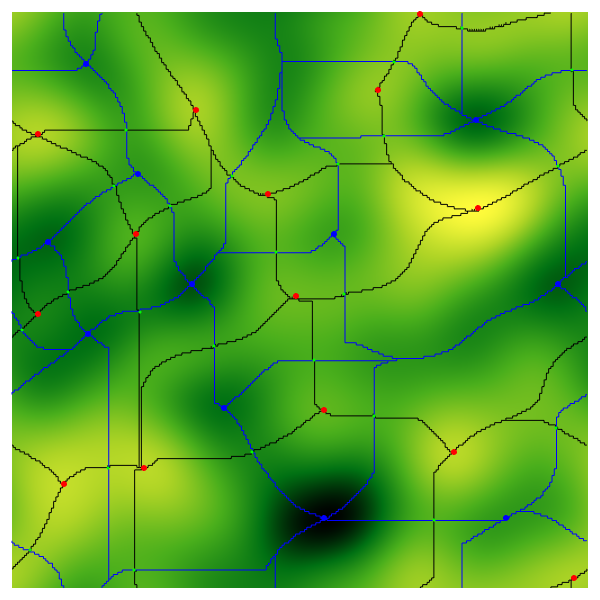
\includegraphics[width=\textwidth]{Visual_GRF}
\caption{The displacement potential}
\label{fig:GRF_MS}
\end{subfigure}
\begin{subfigure}[b]{0.32\textwidth}
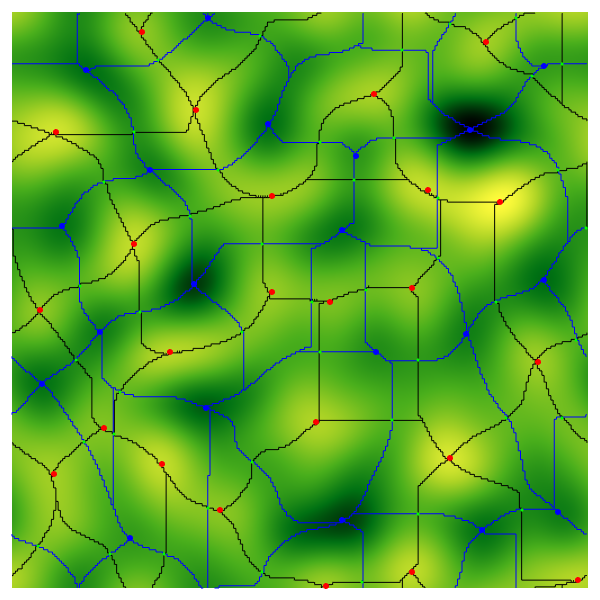
\includegraphics[width=\textwidth]{Visual_dens}
\caption{The density}
\label{fig:dens_MS}
\end{subfigure}
\begin{subfigure}[b]{0.32\textwidth}
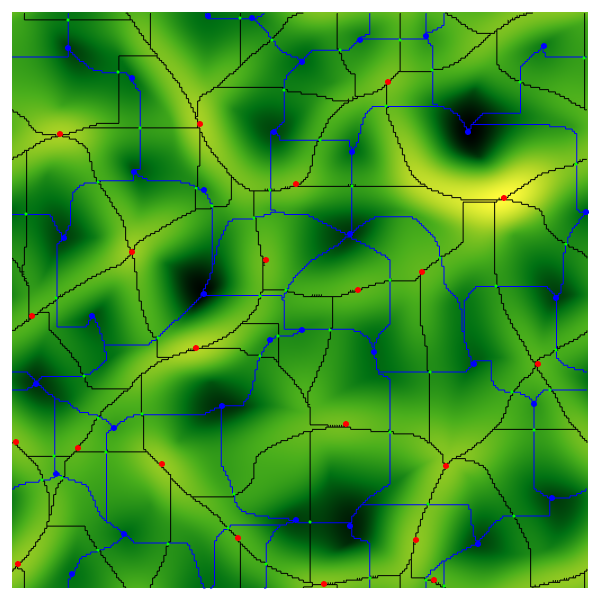
\includegraphics[width=\textwidth]{Visual_eigen1}
\caption{The first eigenvalue field}
\label{fig:eigen1_MS}
\end{subfigure}\\
\begin{subfigure}[b]{0.32\textwidth}
\includegraphics[width=\textwidth]{Visual_Lambda1_D=1}
\caption{The eigenvalue field $b_+=1$}
\label{fig:eigen1_1}
\end{subfigure}
\begin{subfigure}[b]{0.32\textwidth}
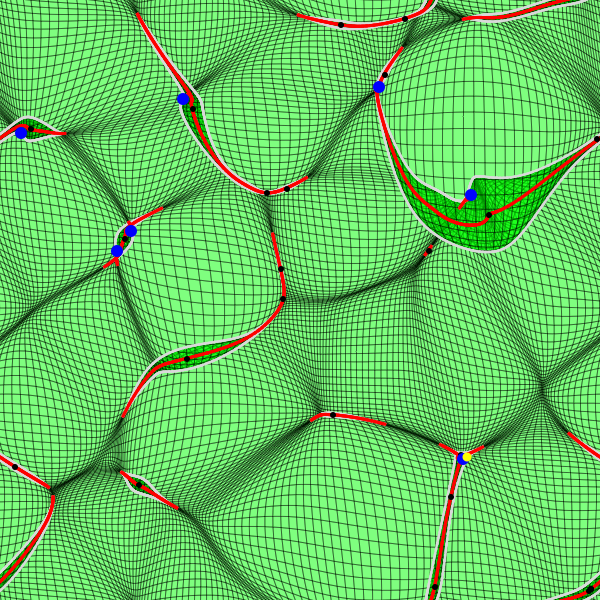
\includegraphics[width=\textwidth]{Visual_Zeldovich_D=1}
\caption{The Zel'dovich flow $b_+=1$}
\label{fig:Zeldovich_1}
\end{subfigure}
\begin{subfigure}[b]{0.32\textwidth}
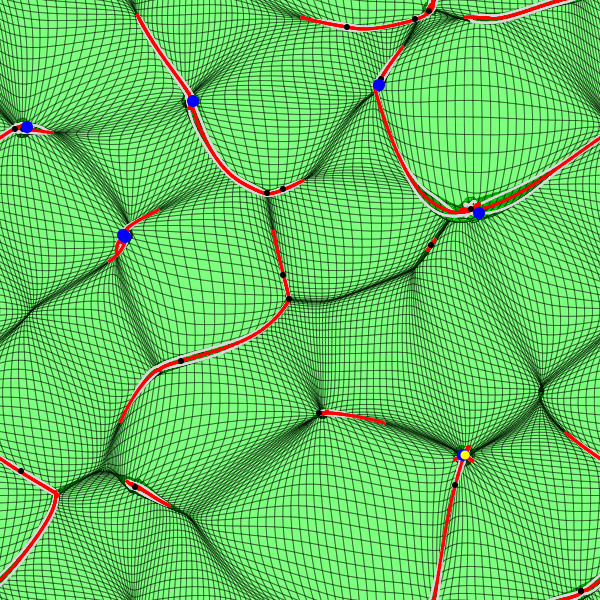
\includegraphics[width=\textwidth]{Visual_Nbody_D=1}
\caption{The $N$-body flow $b_+=1$}
\label{fig:Nbody_1}
\end{subfigure}\\
\begin{subfigure}[b]{0.32\textwidth}
\includegraphics[width=\textwidth]{Visual_Lambda1_D=2}
\caption{The eigenvalue field $b_+=2$}
\label{fig:eigen1_2}
\end{subfigure}
\begin{subfigure}[b]{0.32\textwidth}
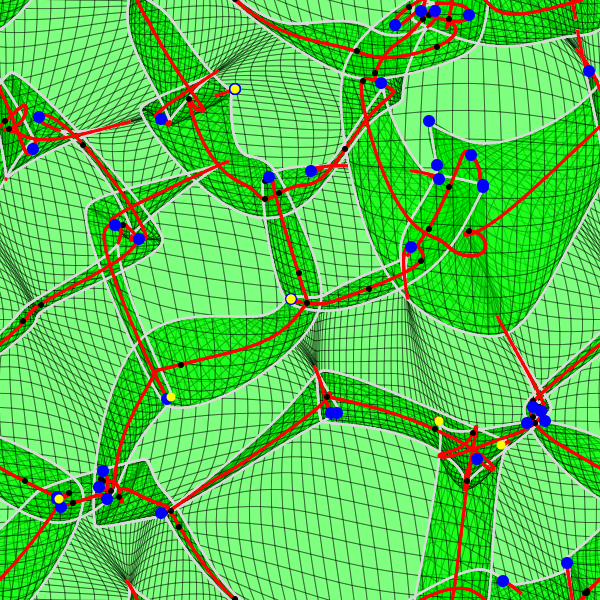
\includegraphics[width=\textwidth]{Visual_Zeldovich_D=2}
\caption{The Zel'dovich flow $b_+=2$}
\label{fig:Zeldovich_2}
\end{subfigure}
\begin{subfigure}[b]{0.32\textwidth}
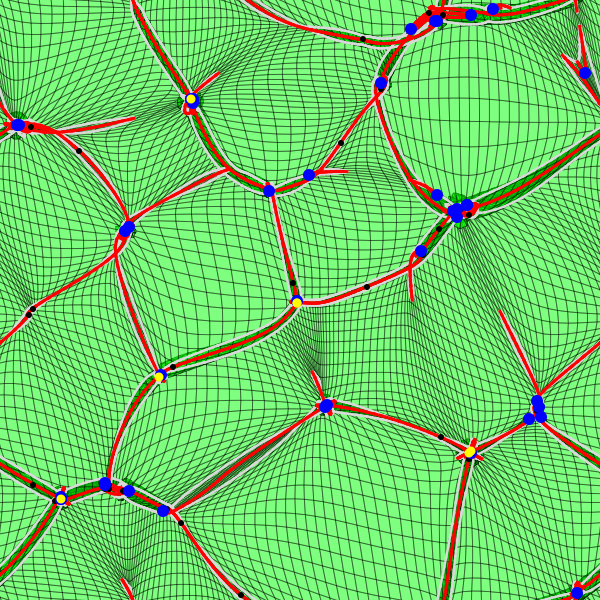
\includegraphics[width=\textwidth]{Visual_Nbody_D=2}
\caption{The $N$-body flow $b_+=2$}
\label{fig:Nbody_2}
\end{subfigure}
\caption{The caustic and the Morse-Smale skeleton. The upper panels show the primordial gravitational potential, the primordial density perturbation and the corresponding eigenvalue field with the Morse-Smale complex. The maxima, saddle points and minima are plotted by the red, green and blue points. The steepest descent and ascent curves corresponding to the saddle points are plotted with the blue and black curves. The lower two rows show the caustic skeleton for growing mode $b_+=1$ and $b_+=2$ in Lagrangian space (left), and Eulerian space (centre and right). The centre figures correspond to the Zel'dovich flow while the right figures correspond to a dark matter $N$-body simulation.}
\label{fig:visualization}
\end{figure}


%%%%%%%%%%%%%%%%%%%%%%%%%%%%%%%%%%%%%%%%%%%%%%%%%%%%%%%%%%%%%%%%
\subsection{Morse-Smale skeleton}
For completeness, we compare the caustic skeleton with the Morse-Smale skeleton which is often used as the definition of the skeleton of the cosmic web. This skeleton is based on the ansatz that the maxima and minima in the primordial density perturbation lead to the clusters, and voids of the cosmic web. In this ansatz, the filaments are associated with the steepest descent curves of the saddle points of the density perturbation field described by the Morse-Smale complex. For completeness, I will here give a concise description of the Morse-Smale complex and the corresponding skeleton.

Given the primordial density perturbation $\delta$, we define the upward flow $\gamma_\lambda$, satisfying the first order differential equation
\begin{align}
\frac{\mathrm{d}}{\mathrm{d}\lambda} \gamma_\lambda(\bm{q}_0) = \nabla \delta(\gamma_\lambda(\bm{q}_0))\,,
\label{eq:MSflow_1}
\end{align}
with the parameter $\lambda \in \mathbb{R}$. For a general point $\bm{q}_0$, the flow satisfying the initial condition
\begin{align}
\gamma_{\lambda=0}(\bm{q}_0) = \bm{q}_0\,,
\end{align}
originates at a minimum (in the limit $\lambda \to -\infty$) and terminates at a maximum (in the limit $\lambda \to + \infty$) of the density perturbation. It is customary to refer to this minimum and maximum as the \textit{origin} and \textit{destination} of the flow corresponding to the point $\bm{q}_0$, \textit{i.e.},
\begin{align}
\textit{org}(\bm{q}_0) &= \lim_{\lambda \to -\infty}\gamma_{\lambda}(\bm{q}_0)\,,\\
\textit{dest}(\bm{q}_0) &= \lim_{\lambda \to +\infty}\gamma_{\lambda}(\bm{q}_0)\,.
\end{align}
We can use these properties to partition Lagrangian space into regions of influence. Given a critical point $\bm{q}_c$, we define the \textit{stable} and the \textit{unstable manifold} by the points that flow towards and originate from the critical point
\begin{align}
S(\bm{q}_c) &= \{\bm{q}_c\} \cup \{ \bm{q}\,|\,\textit{dest}(\bm{q})=\bm{q}_c\}\,,\\
U(\bm{q}_c) &= \{\bm{q}_c\} \cup \{ \bm{q}\,|\,\ \textit{org}(\bm{q})=\bm{q}_c\}\,.
\end{align}
The intersections of these stable and unstable manifolds form the cells of the Morse-Smale complex. Two points in a single Morse-Smale cell share a common origin and destination. The boundaries of cells consist of integral lines, satisfying equation \eqref{eq:MSflow_1}, flowing from the minima to the saddle points and from the saddle points to the maxima of the density perturbation.

In figures \ref{fig:GRF_MS}, \ref{fig:dens_MS}, and \ref{fig:eigen1_MS}, we plot the Morse-Smale complex of the gravitational potential, the density perturbation, and the corresponding first eigenvalue field. The Morse-Smale skeleton consists of the maxima, the minima, and the steepest ascent contours of the saddle points of the primordial density perturbation, corresponding to the clusters, voids, and filaments of the cosmic web (figure \ref{fig:dens_MS}). The Morse-Smale skeleton has strong parallels with the richer caustic skeleton but focuses on the geometry and topology of the initial density perturbation rather than the deformation tensor. We can in fact interpret the caustic skeleton as the Morse-Smale complex of the deformation tensor, as the various caustics mark the points where the deformation tensor exhibits a qualitative change in its structure. The eigenvalue fields take the role of the Morse (height) function.

A visual comparison of the caustic skeleton (figures \ref{fig:eigen1_1} and \ref{fig:eigen1_2}) with the Morse-Smale skeleton (figure \ref{fig:dens_MS}) reveals both strong similarities and differences. The two skeletons agree on large scales. However, the caustic skeleton has generally more detail on smaller scales and includes a larger number of points at which the topology of the cosmic web changes. On a more fundamental level, the definition of the caustic skeleton is tied to the dynamics of Lagrangian fluids while the Morse-Smale skeleton is constructed on a more ad hoc ansatz. Finally note on a more technical level, note that the filaments in the caustic skeleton have a local definition in terms of the gravitational potential. The definition of the filament in the Morse-Smale skeleton is non-local since it is defined in terms of the limit $\lambda\to\infty$ of the flow $\gamma_\lambda$. This makes the filament more difficult to numerically detect and to formally analyse. On the other hand, the statistical properties of the Morse-Smale skeleton can be understood in terms of Gaussian statistics, while the caustic skeleton requires a study of the non-Gaussian eigenvalue and eigenvector fields.


%%%%%%%%%%%%%%%%%%%%%%%%%%%%%%%%%%%%%%%%%%%%%%%%%%%%%%%%%%%%%%%%
\section{The primordial density perturbation}
One of the most startling realizations in modern cosmology is that the intricate cosmic web, observed in several cosmological redshift surveys, originated from an extremely simple initial seed. At the moment of recombination, when the baryons and electrons formed neutral elements and decoupled from the photons, the energy density in our universe $\rho(\bm{q})$, was extremely homogeneous, with the mean density $\bar{\rho}$, containing only tiny perturbations
\begin{align}
\delta(\bm{q}) = \frac{\rho(\bm{q})}{\bar{\rho}} -1\,.
\end{align}
The imprints of these density perturbations in the Cosmic Microwave Background field (CMB) have over the last decades been measured with increasing accuracy. After recombination, the pressure dropped and these small density perturbations started to collapse under the force of gravity leading to the rich geometric patterns in the cosmic web we observe today. The statistics of these initial perturbations $\delta$, is very close to Gaussian. In this section, we describe several properties of Gaussian random fields which are of key importance in this paper. The study of the caustic skeleton presented here can easily be extended to include primordial non-Gaussianities.

%%%%%%%%%%%%%%%%%%%%%%%%%%%%%%%%%%%%%%%%%%%%%%%%%%%%%%%%%%%%%%%%
\subsection{Gaussian random fields}
In cosmology, the density perturbation is a realization of a statistically homogeneous and isotropic three-dimensional random field. In this paper we study a two-dimensional toy model of cosmic structure formation, where the initial density perturbation $\delta:\mathbb{R}^2 \to \mathbb{R}$ has zero mean,
\begin{align}
\langle \delta \rangle 
%&= \left\langle \rho(\bm{q})/\bar{\rho} - 1 \right\rangle\\
= \left\langle \rho(\bm{q}) \right\rangle /\bar{\rho} - 1 =0\,.
\end{align} 
and is a realization of a stationary isotropic Gaussian random field with the distribution
\begin{align}
p(\delta) = e^{-\frac{1}{2} \iint \delta(\bm{q}_1) K(\bm{q}_1,\bm{q}_2) \delta(\bm{q}_2) \mathrm{d}\bm{q}_1 \mathrm{d}\bm{q}_2}\,,
\end{align}
mirroring the Gaussian Euclidean path integral in statistical field theory, \textit{i.e.}, the probability for $\delta$ to be in the set of fields $S$ is given by the Gaussian functional integral
\begin{align}
P[\delta \in S] = \int \bm{1}_S(\delta) e^{-\frac{1}{2} \iint \delta(\bm{q}_1) K(\bm{q}_1,\bm{q}_2) \delta(\bm{q}_2) \mathrm{d}\bm{q}_1 \mathrm{d}\bm{q}_2}\,\mathcal{D}\delta\,,
\end{align}
with $\bm{1}_S$ the identity function with respect to the set $S$ and $\mathcal{D}\delta$ the path integral measure. The expectation value of an observable $Q[\delta]$ is, analogous to quantum physics, given by the insertion of the observable into the path integral
\begin{align} 
\left\langle Q[\delta] \right\rangle = \int Q[\delta]\, e^{-\frac{1}{2} \iint \delta(\bm{q}_1) K(\bm{q}_1,\bm{q}_2) \delta(\bm{q}_2) \mathrm{d}\bm{q}_1 \mathrm{d}\bm{q}_2}\,\mathcal{D}\delta\,.
\end{align}
In these path integrals, the kernel in the exponent $K$ is the inverse of the two-point correlation function $\xi(\bm{q}_1,\bm{q}_2) = \langle \delta(\bm{q}_1) \delta(\bm{q}_2)\rangle$, \textit{i.e.},
\begin{align}
\int \mathrm{d}\bm{q}\, K(\bm{q}_1,\bm{q}) \xi(\bm{q},\bm{q}_2) = \delta_D^{(2)}(\bm{q}_1-\bm{q}_2)\,,
\end{align}
with $\delta_D^{(2)}$ the two-dimensional Dirac delta function. Note that for a statistically homogeneous and isotropic random field, the two-point correlation function only depends on the magnitude of the difference of the points, \textit{i.e.},
\begin{align}
\xi(\bm{q}_1, \bm{q}_2) = \xi(\|\bm{q}_1-\bm{q}_2\|)\,.
\end{align} 

When the set $S$ restricts the density perturbation only at a finite number of spatial points, or when the observable $Q[\delta]$ only depends on the density perturbation at a finite number of points, the functional distribution reduces to the multi-dimensional Gaussian distribution, \textit{i.e.},
\begin{align}
p(\delta(\bm{q}_1), \dots, \delta(\bm{q}_n)) = \frac{\text{Exp}\left[-\frac{1}{2} \sum_{i,j}^n \delta(\bm{q}_i) (M^{-1})_{ij}\delta(\bm{q}_j)\right]}{[(2\pi)^n \det M]^{1/2}}\,,
\end{align}
with the covariance matrix $M$ expressed in terms of the \textit{two-point correlation function} $\xi$,
\begin{align}
[M]_{ij} &= \xi(\|\bm{q}_i - \bm{q}_j\|)\,.
\end{align} 
Linear statistics of the random field $Y=(Y_1,\dots,Y_n)$ follow an analogous distribution
\begin{align}
p(Y) = \frac{\text{Exp}\left[-\frac{1}{2} (Y-\bar{Y})^T M^{-1} (Y-\bar{Y})\right]}{[(2\pi)^n \det M]^{1/2}}\,,
\end{align}
with the mean statistic $\bar{Y} = \langle Y \rangle$ and the covariance matrix $M = \langle Y^T Y \rangle\,.$ Note that the calculations presented in this paper work equally well for more general random fields including non-Gaussianities.

In cosmology, it is convenient to express the two-point correlation function in terms of its Fourier transform, the \textit{power spectrum},
\begin{align}
P_\delta(k) = \int_{-\infty}^{\infty} e^{i k r} \xi(r)\mathrm{d}r\,,
\end{align}
which for a Gaussian random field captures the correlations between the Fourier modes
\begin{align}
\langle \hat{\delta}(\bm{k}_1) \hat{\delta}^*(\bm{k}_2)\rangle = (2\pi)^2 \delta_D^{(2)}(\bm{k}_1-\bm{k}_2) P_\delta(k_1)\,,
\end{align}
with the magnitude $k_1 = \|\bm{k}_1\|$, the two-dimensional Dirac delta function $\delta_D^{(2)}$, and the Fourier transform
\begin{align}
\hat{\delta}(\bm{k}) = \int \delta(\bm{x})e^{i\bm{k}\cdot \bm{x}}\mathrm{d}\bm{x}\,.
\end{align}
Note that correlations of the Fourier modes $\hat{\delta}$ and $\hat{\Psi}$ are diagonal, \textit{i.e.}, the Fourier modes are independently distributed Gaussian variates (taking into account the reality condition $\hat{f}(\bm{k})=\hat{f}^*(-\bm{k})$). We use this property to efficiently generate realizations of unconstrained Gaussian random fields, as detailed in algorithm \ref{alg:GRF} in appendix \ref{ap:GRF}.

It follows from the Poisson equation that the gravitational potential $\phi$ and the displacement potential $\Psi$ inhered the Gaussian statistics of the density perturbations $\delta$. The power spectrum of the displacement potential takes the form 
\begin{align}
P_\Psi(k) &= 16 \pi^2 G^2 \rho_0^2 \frac{P_\delta(k)}{k^4}%\\
%&= \frac{9 \Omega_0^2 H_0^2}{4} \frac{P_\delta(k)}{k^4}
\,.
\end{align}
The statistical properties of these random fields are often conveniently expressed in terms of the moments
\begin{align}
\sigma_i^2 &= \frac{1}{(2\pi)^2} \int k^{2i}P_\delta(k)\mathrm{d}\bm{k}\nonumber\\
&= \frac{1}{2\pi} \int_0^\infty k^{2i}P_\delta(k)\mathrm{d}k\,,
\end{align}
with the magnitude $k = \|\bm{k}\|$, a generalization of the variance of the field
\begin{align}
\sigma_0^2 = \langle \delta^2(\bm{q}) \rangle\,.
\end{align} 
The moments of the displacement potential are directly related to the moments of the density perturbation
\begin{align}
\tau_i^2&=\frac{1}{(2\pi)^2} \int k^{2i}P_\Psi(k)\mathrm{d}\bm{k}\nonumber\\
&=16 \pi^2 G^2 \rho_0^2 \sigma_{i-2}^2\,.
\end{align}
In appendix \ref{ap:correlations} we list closed form expressions for the moments used in this paper.


%%%%%%%%%%%%%%%%%%%%%%%%%%%%%%%%%%%%%%%%%%%%%%%%%%%%%%%%%%%%%%%%
\subsection{Scale space}
The cosmic web is a fractal like structure spanning an enormous range of scales. To trace this fractal nature, we study the cosmic web in scale space with the smoothed initial density perturbation
\begin{align}
\delta(\bm{q},R) = \int \delta(\bm{q}') W_R(\|\bm{q}' - \bm{q}\|)\,,
\end{align}
at scale $R$. In this paper we, for convenience, use the Gaussian window function
\begin{align}
W_R(r) = \frac{1}{\sqrt{2\pi R^2}}e^{-\frac{r^2}{2R^2}}\,.
\end{align}
This choice is not fundamental to our approach but simplifies the equations. Note that, using the convolution theorem, 
\begin{align}
\hat{\delta}(\bm{q},R) = \hat{\delta}(\bm{q})  \hat{W}_R(r)\,,
\end{align}
with the Fourier transform
\begin{align}
\hat{W}_R(k) = e^{-\frac{R^2 k^2}{2}}\,,
\end{align}
we can interpret the smoothed field $\delta(\bm{q},R)$ as a realization of a Gaussian random field with the power spectrum
\begin{align}
P_\delta(k) \mapsto \hat{W}_R(k)^2P_\delta(k)\,.
\end{align}

%%%%%%%%%%%%%%%%%%%%%%%%%%%%%%%%%%%%%%%%%%%%%%%%%%%%%%%%%%%%%%%%
\subsection{Constrained Gaussian random fields}\label{sec:ConstrainedGRFs}
In this paper, we study the ways in which different features of the cosmic web emerge from different patches of the Gaussian initial conditions. In order to study these patches in detail, we use constrained Gaussian random field theory following the analysis of [van de Weygaert and Bertschinger 1996]. We first summarize the theory of constrained Gaussian random fields with linear constraints. We subsequently extend the theory to a wide class of non-linear constraints.

%%%%%%%%%%%%%%%%%%%%%%%%%%%%%%%%%%%%%%%%%%%%%%%%%%%%%%%%%%%%%%%%
\subsubsection{Linear constraints}
For a random field $f$, let's consider the linear constraints
\begin{align}
C_i[f;\bm{q}_i] = c_i\,,
\end{align}
for $i=1,\dots,n$. The linear constraints can take the form of the function value, a derivative, or a convolution
\begin{align}
C[f;\bm{q}'] &= f(\bm{q}')\,,\\
C[f;\bm{q}'] &= \frac{\partial}{\partial q_i}f(\bm{q}')\,,\\
C[f;\bm{q}'] &= \int g(\bm{q}' - \bm{q})f(\bm{q})\mathrm{d}\bm{q}\,.
\end{align}

A constrained realization $f$ can be expressed as the sum
\begin{align}
f(\bm{q}) = \bar{f}(\bm{q}) + F(\bm{q})\,,
\end{align}
with the mean field $\bar{f}$ and the residue $F$. The mean field is defined as
\begin{align}
\bar{f}(\bm{q}) 
&= \left\langle f(\bm{q})|C_i[f;\bm{q}_i]=c_i \right\rangle\nonumber\\
&= \sum_{i,j=1}^n \xi_i(\bm{q}) \xi^{-1}_{ij} c_j\,,
\end{align}
where the cross-correlation between the random field and the constraints, and the cross-correlation of the constraints are defined as
\begin{align}
\xi_i(\bm{q}) &= \left\langle f(\bm{q}) C_i[f;\bm{q}_i]\right\rangle\,,\\
\xi_{ij} &= \langle C_i C_j \rangle\,.
\end{align}
In appendix \ref{ap:correlations}, we list closed form expressions for the correlation functions used in this paper. 

The mean field satisfies the consistency relation $C_i[\bar{f};\bm{q}_i]=c_i$, while the residue field $F$ vanishes on the constraint, $C_i[F;\bm{q}_i]=0$. For linear constraints, the residue $F$ turns out to be completely independent of the actual values of the constraints $c_i$. The Hoffman-Ribak method exploits this property to generate realizations of Gaussian random fields with linear constraints (see algorithm \ref{alg:HoffmanRibak} in appendix \ref{ap:GRF}). The variance of the residue takes the form
\begin{align}
\left\langle F(\bm{q})^2|C_i[f;\bm{q}_i]=c_i \right\rangle = \sigma_0^2 - \sum_{i,j=1}^n\xi_i(\bm{q}) \xi_{ij}^{-1} \xi_j(\bm{q})\,,
\end{align}
with the variance of the unconstrained field $\sigma_0^2 = \langle f(\bm{q})^2\rangle$. Note that the variance of the residue is independent of the values of the constraints $c_i$.

%%%%%%%%%%%%%%%%%%%%%%%%%%%%%%%%%%%%%%%%%%%%%%%%%%%%%%%%%%%%%%%%
\subsubsection{Non-linear constraints}
For the caustic skeleton, we will consider more general non-linear constraints. Consider a set of $n$ constraints $\mathcal{C}_i(T_{ij\dots k}) = 0$, consisting of functions in terms of a finite number of derivatives of the displacement potential $T_{ij\dots k}$. These conditions span a constraint manifold in the space of derivatives of the displacement potential
\begin{align}
\mathcal{M}_{\mathcal{C}} = 
\{(T_{ij\dots})|\mathcal{C}_j=0 \text{ for } j = 1, 2, \dots ,n\}\,.
\end{align}
For example, consider the condition on the first eigenvalue field
\begin{align}
\mathcal{C}(\lambda_i,\bm{v}_i) = \lambda_1 - \lambda\,,
\end{align}
with the constraint manifold (see figure \ref{fig:ConstrainedManifold})
\begin{align}
\mathcal{M}_\mathcal{C}=\left\{(T_{11},T_{12},T_{22})\bigg| \lambda = \frac{1}{2}\left(T_{11}+T_{22} + \sqrt{4 T_{12}^2 + (T_{11}-T_{22})^2}\right)\right \} \,.
\label{eq:exampleConstrainedManifold}
\end{align}


\begin{figure}
\centering
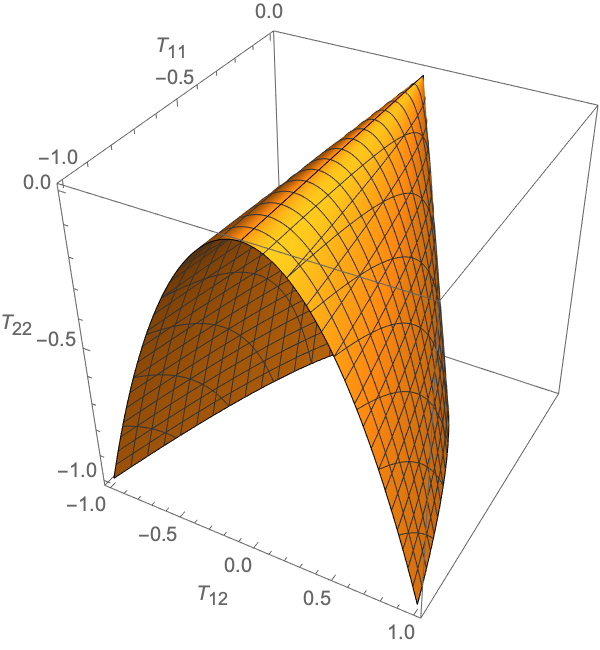
\includegraphics[width=0.5\textwidth]{ConstraintManifold}
%\begin{tikzpicture}[xscale=0.8,>=latex,scale=0.6]
%% axis
%\draw[ thick,->] (0.3,-3.5) -- +(0,7) node[yshift=7pt] {$T_{11}$};
%\draw[ thick,->] (0.3,-3.5) -- +(220:4) node[yshift=-5pt,xshift=-5pt] {$T_{12}$};
%\draw[ thick,->] (0.3,-3.5) -- +(10,0) node[xshift=10pt] {$T_{22}$};
%
%\shade[top color=gray!10,bottom color=gray!90,opacity=.90] 
%  (-1,-4) to[out=20,in=220] (3,3)  to[out=10,in=140] (9,1)
% to[out=210,in=40] (6,-7) to[out=80,in=0] (-1,-4);
% 
%% labels
%\node at (9.4,-4.5) (label) {$\mathcal{M}_{\mathcal{C}}$};
%\draw[->] (label) -- +(185:3.35);
%
%% border of the surface
%\path[draw,name path=border3] (-1,-4) to[out=20,in=220] (3,3);
%\path[draw,name path=border4] (6,-7) to[out=40,in=210] (9,1);
%\path[draw,name path=border5] (-1,-4) to[out=0,in=80] (6,-7);
%\path[draw,name path=border6] (3,3) to[out=10,in=140] (9,1);
%\end{tikzpicture}
\caption{The constraint manifold $\mathcal{M}_\mathcal{C}$ in the space of derivatives of the deformation tensor corresponding to equation \eqref{eq:exampleConstrainedManifold}.}
\label{fig:ConstrainedManifold}
\end{figure}

Using Bayes' rule, the distribution of points on the constraint manifold $\bm{c} \in \mathcal{M}_{\mathcal{C}}$ is proportional to the original Gaussian distribution
\begin{align}
p(\bm{c}\,|\,\bm{c}\in \mathcal{M}_{\mathcal{C}})  = \frac{p(\bm{c})}{\int_{\mathcal{M}_\mathcal{C}} p(\bm{c})\, \mathrm{d}\bm{c}}\,.
\end{align}
For every point $\bm{c}$ on the manifold $\mathcal{M}_{\bm{c}}$, we can use the theory of linear constrained Gaussian random fields to analyse the mean field and the residue. That is to say, for a sample $\bm{c} \in \mathcal{M}_\mathcal{C}$, we can use the Hoffman-Ribak method to generate a realization (algorithm \ref{alg:HoffmanRibak} in appendix \ref{ap:GRF}). The problem of generating a constraint realization with non-linear constraints is thus reduced to sampling points on the constraint manifold.

Conversely, given the mean field $\bar{f}_{\bm{c}}$, corresponding to the instance $\bm{c} \in \mathcal{M}_{\mathcal{C}}$, we can evaluate the mean field corresponding to the constraints $\mathcal{C}$ by integrating over the constraint manifold, \textit{i.e.},
\begin{align}
\bar{f}_{\mathcal{C}}(\bm{q}) 
&=\left\langle f(\bm{q})|\mathcal{C}\right \rangle \nonumber\\
&= \int_{\bm{c} \in \mathcal{M}_{\mathcal{C}}} \bar{f}_{\bm{c}}(\bm{q})\, p(\bm{c}|\bm{c}\in \mathcal{M}_{\mathcal{C}}) \mathrm{d}\bm{c}\nonumber\\
&= \sum_{i,j=1}^n\xi_i(\bm{q}) \xi_{ij}^{-1}\int_{\bm{c} \in \mathcal{M}_{\mathcal{C}}}  c_i\, p(\bm{c}|\bm{c}\in \mathcal{M}_{\mathcal{C}}) \mathrm{d}\bm{c}\nonumber\\
&= \sum_{i,j=1}^n \xi_i(\bm{q}) \xi_{ij}^{-1} \bar{c}_i\nonumber\\
&= \bar{f}_{\bar{\bm{c}}}(\bm{q})\,,
\end{align}
with the mean constraint
\begin{align}
\bar{\bm{c}} &\equiv \langle \bm{c} \,|\, \mathcal{C}\rangle = \int_{\bm{c} \in \mathcal{M}_{\mathcal{C}}}  \bm{c}\, p(\bm{c}\,|\,\bm{c}\in \mathcal{M}_{\mathcal{C}}) \mathrm{d}\bm{c}\,.
\end{align}
The evaluation of the mean field of a set of non-linear constraints has thus been reduced to evaluating the expectation values of the constraints with respect to the constraint manifold. Since the distribution $p(\bm{c}\,|\,\bm{c}\in \mathcal{M}_{\mathcal{C}})$ has an explicit form, we can either perform these calculations exactly with analytic or numerically with Monte Carlo methods.

The variance of the corresponding residue, $F = f - \bar{f}_{\mathcal{C}}$, coincides with the variance of residue of the corresponding constraint problem with linear constraints,
\begin{align}
\left \langle F(\bm{q})^2\,|\,\mathcal{C}\right\rangle &= \int_{\mathcal{M}_\mathcal{C}} \langle F(\bm{q})^2\, |\, \bm{c}\rangle\, p(\bm{c}\,|\, \bm{c} \in \mathcal{M}_\mathcal{C})\mathrm{d}\bm{c}\nonumber\\
&=\int_{\mathcal{M}_\mathcal{C}} 
\left( \tau_0^2 - \sum_{i,j=1}^n\xi_i(\bm{q}) \xi_{ij}^{-1} \xi_j(\bm{q})\right) p(\bm{c}\,|\,\bm{c}\in \mathcal{M}_\mathcal{C})\,\mathrm{d}\bm{c}\nonumber\\
&= \tau_0^2 - \sum_{i,j=1}^n\xi_i(\bm{q}) \xi_{ij}^{-1} \xi_j(\bm{q})\,,
\end{align}
since the variance of the linear constraint problem is independent of the value of the constraint and the variance of the sum of two distributions is the sum of their variances. 

%%%%%%%%%%%%%%%%%%%%%%%%%%%%%%%%%%%%%%%%%%%%%%%%%%%%%%%%%%%%%%%%
\section{The statistical properties of the caustic skeleton}\label{sec:causticSkeleton}
We can use the definition of the caustic skeleton in terms of the eigenvalue and eigenvector fields of the deformation tensor and the details of Gaussian random field theory to evaluate the statistical properties of the various elements of the caustic skeleton in Lagrangian space. For more detailed expressions in terms of the distribution of the underlying Gaussian random field see appendix \ref{ap:explicitFroms}.




%%%%%%%%%%%%%%%%%%%%%%%%%%%%%%%%%%%%%%%%%%%%%%%%%%%%%%%%%%%%%%%%
\subsection{Collapsed regions}
The fold manifold is intimately related to the eigenvalue fields which are distributed according to the two-dimensional Doroshkevich formula (see appendix \ref{ap:Doreskevish} for a derivation)
\begin{align}
p(\lambda_1, \lambda_2) = \frac{2\sqrt{2}}{\pi^{1/2}\tau_2^3} e^{-\frac{3(\lambda_1+\lambda_2)^2 - 8 \lambda_1 \lambda_2}{2 \tau_2^2}}(\lambda_1 - \lambda_2)\,.
\end{align}
See figure \ref{fig:Doroshkevich} for an illustration of this joined distribution.
\begin{figure}
\centering
\begin{subfigure}[b]{0.4\textwidth}
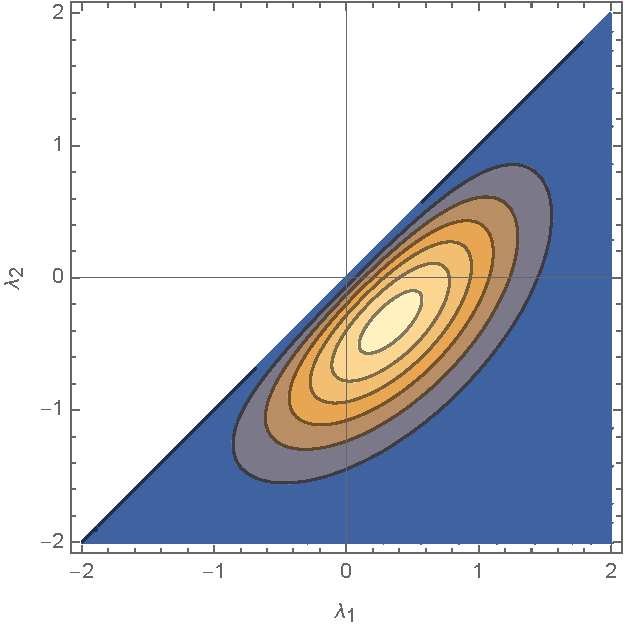
\includegraphics[width=\textwidth]{Doroshkevich}
\caption{The joint distribution of the eigenvalue fields of a Gaussian random field.\\}
\label{fig:Doroshkevich}
\end{subfigure}
\begin{subfigure}[b]{0.4\textwidth}
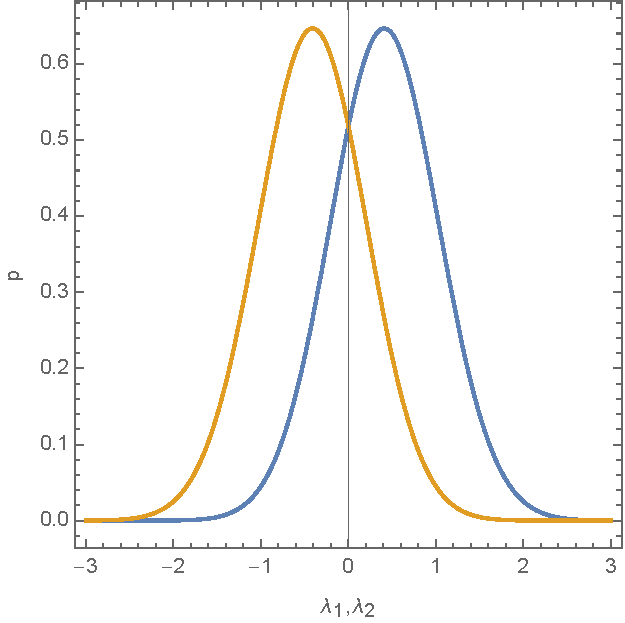
\includegraphics[width=\textwidth]{Eigenvalues}
\caption{The marginal distribution of the eigenvalue fields of a Gaussian random field (blue and yellow correspond to $\lambda_1$ and $\lambda_2$).}
\label{fig:eigenvalues}
\end{subfigure}
\caption{The distribution of eigenvalue fields in a Gaussian random field with the moment $\tau_2=1$.}
\end{figure}
The marginal distributions of the two eigenvalues are given by
\begin{align}
p(\lambda_1) &= 
\frac{1}{9\tau_2^2} e^{-\frac{2 \lambda_1^2}{\tau_2^2}}\left(
6 \sqrt{\frac{2}{\pi}} \tau_2 + 4 \sqrt{3} e^{\frac{2\lambda_1^2}{3\tau_2^2}}\lambda_1\left(1+\text{Erf}\left[\sqrt{\frac{2}{3}}\frac{1}{\tau_2} \lambda_1\right]\right)
\right)\,,\\
p(\lambda_2) &= 
\frac{1}{9\tau_2^2} e^{-\frac{2 \lambda_2^2}{\tau_2^2}}\left(
6 \sqrt{\frac{2}{\pi}} \tau_2 + 4 \sqrt{3} e^{\frac{2\lambda_2^2}{3\tau_2^2}}\lambda_2\text{Erfc}\left[\sqrt{\frac{2}{3}}\frac{1}{\tau_2} \lambda_2\right]\right)\,.
\end{align}
See Fig.\ \ref{fig:eigenvalues} for an illustration of the marginal distributions.

The percentage of the mass, and thus Lagrangian space, having experienced a single or two shell-crossings in the Zel'dovich approximation at a given time $t_0$, with $b_+(t_0)=b_+$, is given by
\begin{align}
\mathcal{A}[A_2^1] 
&= \int_{1/b_+(t)}^\infty p(\lambda_1) \mathrm{d}\lambda_1\nonumber\\
&= \frac{1}{6}\left(
\sqrt{3}e^{-\frac{4}{3b_+^2\tau_2^2}}\left(1+\text{Erf}\left[\sqrt{\frac{2}{3}}\frac{1}{b_+\tau_2}\right]\right) + 3 \,\text{Erfc}\left[\frac{\sqrt{2}}{b_+ \tau_2}\right]
\right)\,,\\
\mathcal{A}[A_2^1] 
&= \int_{1/b_+(t)}^\infty p(\lambda_2) \mathrm{d}\lambda_2\nonumber\\
&= \frac{1}{6}\left(
-\sqrt{3}e^{-\frac{4}{3b_+^2\tau_2^2}}\text{Erfc}\left[\sqrt{\frac{2}{3}}\frac{1}{b_+\tau_2}\right] + 3 \,\text{Erfc}\left[\frac{\sqrt{2}}{b_+ \tau_2}\right]\right)\,.
\end{align}
The percentage of the mass not having collapsed in the Zel'dovich approximation, most likely residing in the voids, is given by $1-\mathcal{A}[A_2^1]$. In the limit of $b_+(t) \to \infty$, 
\begin{align}
\mathcal{A}[A_2^1]  \to \frac{1}{2} + \frac{\sqrt{3}}{6}\,,\quad
\mathcal{A}[A_2^2]  \to \frac{1}{2} - \frac{\sqrt{3}}{6}\,.
\end{align}
These identities are independent of the power spectrum of the random field. Note that in a $\Lambda$CDM universe, the growing mode does not grow indefinitely. See Fig.\ \ref{fig:A2} for an illustration of the percentage of the mass in the filaments and clusters as a function of the growing mode $b_+$.

The line-length density of the shell-crossing region for a given eigenvalue is given by the expectation value
\begin{align}
L(A_2^i) = \left\langle \| \nabla \lambda_i\|\, \delta_D^{(1)}(\lambda_i - \lambda)\right \rangle\,.
\end{align}
The line length of the fold caustic is in particular of interest in optical systems. See appendix \ref{ap:explicitFroms} for detailed discussion.


\begin{figure}
\centering
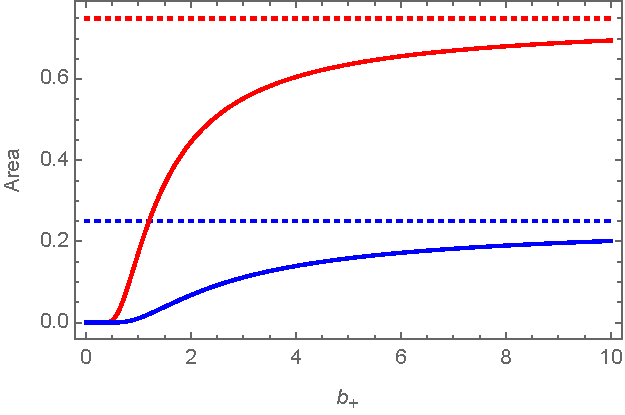
\includegraphics[width=0.5\textwidth]{A2Area}
\caption{The percentage of the mass elements having undergone a single $\mathcal{A}[A_2^1]$ (red) or two $\mathcal{A}[A_2^2]$ (blue) shell-crossings in the Zel'dovich approximation for $\tau_2=1$. The solid curves correspond to the evolution as a function of the growing mode $b_+$. The horizontal dotted lines correspond to the corresponding limits.}
\label{fig:A2}
\end{figure}

The shell-crossing regions $A_2^i(t)$ changes topology at the critical points of the eigenvalue fields. The number densities of these points at eigenvalue field $\lambda$ are given by Rice's formula
\begin{align}
\mathcal{N}_{\lambda_i}(\lambda) 
&= \left \langle 
|\det \mathcal{H} \lambda_i |\, \delta_D^{(1)}(\lambda_i - \lambda)\, \delta_D^{(2)}(\nabla \lambda_i)
\right \rangle\nonumber \\
&= \left \langle 
\left|\lambda_{i,11}\lambda_{i,22} -\lambda_{i,12}^2\right|\, 
\delta_D^{(1)}(\lambda_i - \lambda)\, 
\delta_D^{(2)}(\nabla \lambda_i)
\right \rangle \,,
\end{align}
with the Hessian operator $[\mathcal{H}]_{ij}=\frac{\partial^2}{\partial q_i \partial q_j}$, and the partial derivatives $\lambda_{i,jk}=\frac{\partial^2}{\partial q_j \partial q_k} \lambda_i$ (see appendix \ref{ap:stochasticGeometry} for a discussion of Rice's formula). We can evaluate the point density of the maxima, minima, and saddle points by restricting the integration domain to the regions where the Hessian, $\mathcal{H} \lambda_i$, is negative definite, positive definite, and has a negative determinant (see the left and the right panels of figure \ref{fig:EigenvalueCriticalPoints}). Note that the maxima and minima of the eigenvalue fields are not symmetric reflecting the non-Gaussian nature of the eigenvalue fields. We should contrast this with the distribution of critical points of the Gaussian density perturbation (see figure \ref{fig:delta_critical}), 
\begin{align}
\mathcal{N}_{\delta}(\lambda) 
&= \left \langle 
|\det \mathcal{H} \delta |\, \delta_D^{(1)}(\delta - \lambda)\, \delta_D^{(2)}(\nabla \delta)
\right \rangle\nonumber\\
&= \left \langle 
|\delta_{,11}\delta_{,22}-\delta_{,12}^2 |\, \delta_D^{(1)}(\delta - \lambda)\, \delta_D^{(2)}(\nabla \delta)
\right \rangle\,.
\end{align}

\begin{figure}
\centering
\begin{subfigure}[b]{0.32\textwidth}
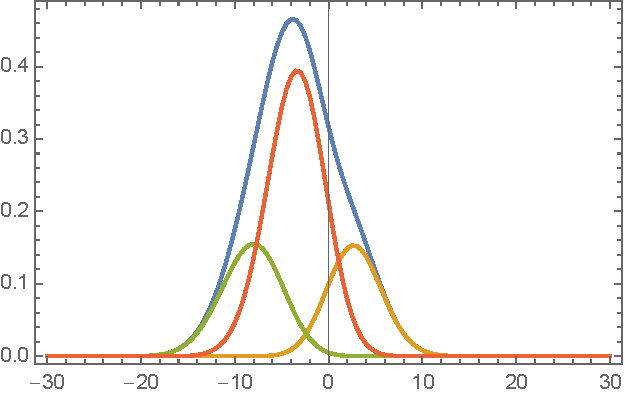
\includegraphics[width=\textwidth]{Lambda2Density}
\caption{The number density of critical points corresponding to the second eigenvalue field $\lambda_2$. All critical points (blue), the minima (green), the saddle points (orange), and the maxima (yellow).}
\end{subfigure}
\begin{subfigure}[b]{0.32\textwidth}
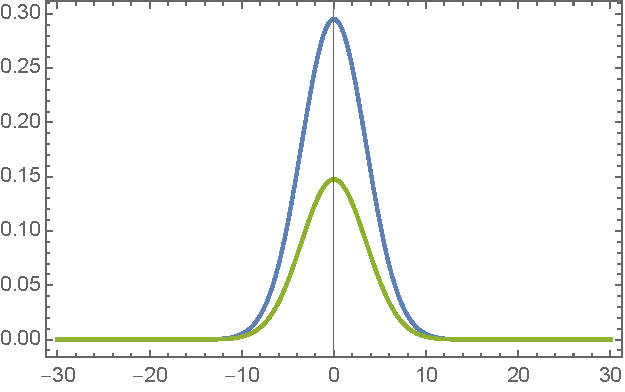
\includegraphics[width=\textwidth]{D4Density}
\caption{The number density of umbilic points $D_4^{\pm}$. All umbilic points points $D_4^{\pm}$ (blue) and the individual distributions $D_4^+$ and $D_4^-$ (green).\\$ $\\}
\end{subfigure}
\begin{subfigure}[b]{0.32\textwidth}
\includegraphics[width=\textwidth]{Lambda1Density}
\caption{The number density of critical points corresponding to the first eigenvalue field $\lambda_1$. All critical points (blue), the minima (yellow), the saddle points (orange), and the maxima (green).\\}
\end{subfigure}
\caption{The number density of topological points in the eigenvalue fields of the deformation tensor as a function of the eigenvalue field.}
\label{fig:EigenvalueCriticalPoints}
\end{figure}

The topology of the fold manifold also changes at the umbilic points $D_4^\pm$ where the two eigenvalue fields coincide, \textit{i.e.}, $T_{11}=T_{22}=\lambda$ and $T_{12}=0$. The number density of umbilic points is given by
\begin{align}
\mathcal{N}_{D_4^\pm}(\lambda) =& 
\left \langle \left|\det\left(\nabla (T_{11}-T_{22}), \nabla (T_{12})\right)\right|\, 
\delta_D^{(1)}(T_{11} - \lambda)\, 
\delta_D^{(1)}(T_{11}-T_{22})\, 
\delta_D^{(1)}(T_{12}) \right \rangle\,,
\end{align}
plotted in the central panel of figure \ref{fig:EigenvalueCriticalPoints}. For a more detailed description of the umbilic points see section \ref{sec:clustersStats}.


\begin{figure}
\centering
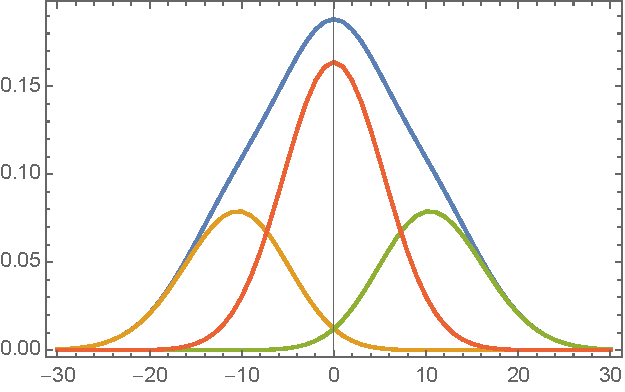
\includegraphics[width=0.5\textwidth]{DensityDensity}
\caption{The number density of critical points of the density perturbation. All critical points (blue), the minima (yellow), the saddle points (red), and the maxima (green) as a function of the density perturbation. }
\label{fig:delta_critical}
\end{figure}

%%%%%%%%%%%%%%%%%%%%%%%%%%%%%%%%%%%%%%%%%%%%%%%%%%%%%%%%%%%%%%%%
\subsection{Filaments}
The line length density per unit of area of the cusp curves in Lagrangian space is the expectation value (for details see appendix \ref{ap:stochasticGeometry})
\begin{align}
\mathcal{L}(A_3^i) 
&=  \left \langle \| \nabla (\bm{v}_i \cdot \nabla \lambda_i) \|\,
\delta_D^{(1)}(\lambda_i-\lambda)\,
\delta_D^{(1)}(\bm{v}_i \cdot \nabla \lambda_i) \right \rangle \,,
\end{align}
where $\mathcal{L}(A_3^i)$ is the differential of the length $\frac{\mathrm{d}}{\mathrm{d}\lambda} L(A_3^i)$.
See figure \ref{fig:A3LengthDensity} for an illustration of the line length density of the cusp curve corresponding to the first and the second eigenvalue fields.
\begin{figure}
\centering
\begin{subfigure}[b]{0.32\textwidth}
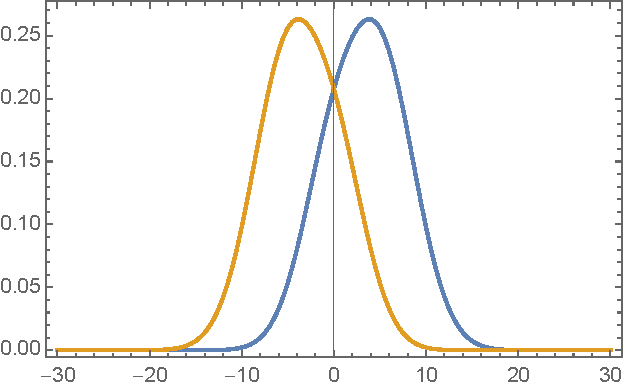
\includegraphics[width=\textwidth]{A3LengthDensity}
\caption{The line length density of the cusp curve $A_3^i$ corresponding to the first (red) and the second eigenvalue field (blue).\\}
\end{subfigure}
\begin{subfigure}[b]{0.32\textwidth}
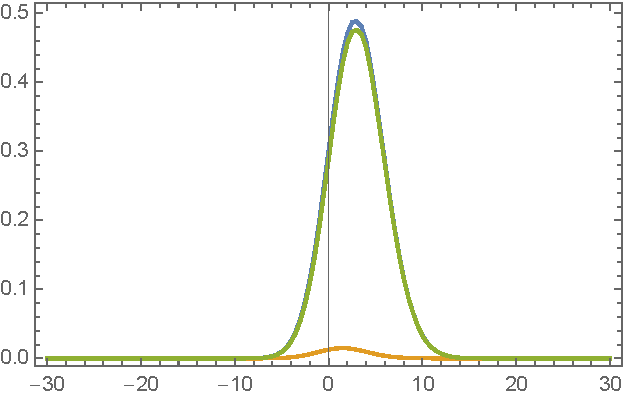
\includegraphics[width=\textwidth]{A3NumberDensity_1}
\caption{The number density of the cusp points $A_3^{1\pm}$ corresponding to the first eigenvalue fields. The total (black) the creation (red) and merger events (blue).}
\end{subfigure}
\begin{subfigure}[b]{0.32\textwidth}
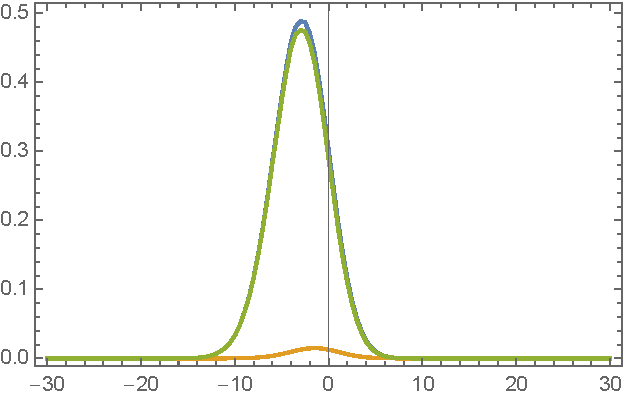
\includegraphics[width=\textwidth]{A3NumberDensity_2}
\caption{The number density of the cusp points $A_3^{2\pm}$ corresponding to the second eigenvalue fields. The total (black) the creation (red) and merger events (blue).}
\end{subfigure}
\caption{The statistics of the cusp lines $A_3^i$.}

\label{fig:A3LengthDensity}
\end{figure}

The Morse points, $A_3^{i\pm}$, where the topology of the cusp curve changes, are defined as the maxima and minima of the eigenvalue field $\lambda_i$ restricted to the cusp curve $A_3^i$. Since the $A_3^i$ curve is defined as the zero set $\bm{v}_i \cdot \nabla \lambda_i=0$, the normal to the normal direction to the $A_3^i$ curve is defined as the gradient $\nabla(\bm{v}_i \cdot \nabla \lambda_i)$. The derivative of the eigenvalue field $\lambda_i$ in the direction of the $A_3^i$ curve can thus be expressed as $(\nabla(\bm{v}_i \cdot \nabla \lambda_i))^\perp \cdot \nabla \lambda_i$, with the normal $\bm{v}^\perp$  of the vector $\bm{v}$, \textit{i.e.}, for the vector $\bm{v}=(a,b)\in \mathbb{R}^2$ we define the normal vector as $\bm{v}^\perp = (-b,a) \in \mathbb{R}^2$. The second order derivative of the eigenvalue field $\lambda_i$ in the direction of the $A_3^i$ curve is given by $(\nabla(\bm{v}_i \cdot \nabla \lambda_i))^\perp \cdot\nabla((\nabla(\bm{v}_i \cdot \nabla \lambda_i))^\perp \cdot \nabla \lambda_i)$. Using these identities, we can express the number density of these Morse points as the expectation value
\begin{align}
\mathcal{N}(A_3^{i\pm}) 
= \bigg \langle &\left|\det\left(\nabla (\bm{v}_i \cdot \nabla \lambda_i), \nabla ((\nabla (\bm{v}_i \cdot \nabla \lambda_i))^\perp \cdot \nabla \lambda_i)\right)\right|\,
 \delta_D^{(1)}(\lambda_i - \lambda)\,
  \delta_D^{(1)}(\bm{v}_i \cdot \nabla \lambda_i) \nonumber\\
&\delta_D^{(1)}((\nabla(\bm{v}_i \cdot \nabla \lambda_i))^\perp \cdot \nabla \lambda_i)) \bigg \rangle\,,
\end{align}
where the integration domain for the creation and merger points are determined by the sign
\begin{align}
\text{sign}\left[
(\nabla (\bm{v}_i \cdot \nabla \lambda_i))^\perp \cdot \nabla ((\nabla (\bm{v}_i \cdot \nabla \lambda_i))^\perp \cdot \nabla \lambda_i)
\right]=\pm 1\,.
\end{align}
For the cusp points, the determinant in the expectation value happens to coincide with the second order derivative of the eigenvalue field in the direction of the $A_3^i$ curve. For in illustration of the Morse point densities see figure \ref{fig:A3LengthDensity}.

%%%%%%%%%%%%%%%%%%%%%%%%%%%%%%%%%%%%%%%%%%%%%%%%%%%%%%%%%%%%%%%%
\subsection{Clusters}\label{sec:clustersStats}
The number density of swallowtail points is given by the expectation 
\begin{align}
\mathcal{N}(A_4^{i}) 
=&\,\bigg \langle \left|\det\left(\nabla (\bm{v}_i \cdot \nabla \lambda_i), \nabla (\bm{v}_i \cdot \nabla(\bm{v}_i \cdot \nabla \lambda_i)\right)\right|\,
 \delta_D^{(1)}(\lambda_i - \lambda)\,
  \delta_D^{(1)}(\bm{v}_i \cdot \nabla \lambda_i) \nonumber\\
&\delta_D^{(1)}(\bm{v}_i \cdot \nabla(\bm{v}_i \cdot \nabla \lambda_i)) \bigg \rangle\\
=&\, \bigg \langle \left| \left[\bm{v}_j \cdot \nabla (\bm{v}_i \cdot \nabla \lambda_i)\right]\left[ \bm{v}_i \cdot \nabla (\bm{v}_i \cdot \nabla(\bm{v}_i \cdot \nabla \lambda_i))\right]\right|\,
 \delta_D^{(1)}(\lambda_i - \lambda)\,
  \delta_D^{(1)}(\bm{v}_i \cdot \nabla \lambda_i) \nonumber\\
&\delta_D^{(1)}(\bm{v}_i \cdot \nabla(\bm{v}_i \cdot \nabla \lambda_i)) \bigg \rangle\,.
\end{align}
with $i\neq j$. The number density of umbilic points is given by the Gaussian distribution
\begin{align}
\mathcal{N}(D_4^{12\pm}) 
=&\, \left \langle \left|\det\left(\nabla (T_{11}-T_{22}), \nabla (T_{12})\right)\right|\,
 \delta_D^{(1)}(T_{11} - \lambda)\,
  \delta_D^{(1)}(T_{11}-T_{22})\,
  \delta_D^{(1)}(T_{12}) \right \rangle\nonumber\\
\propto &\, e^{-\frac{2 \lambda^2}{\tau_2^2}} \,.
\end{align}
The number density of the hyperbolic and elliptic umbilic points can be obtained by restricting the integration domain for which the sign of the determinant which coincides with $\mathcal{S}_\mathcal{M}$. From symmetry arguments, it follows that the hyperbolic and elliptic caustics are equally likely to be realized, \textit{i.e.},
\begin{align}
\mathcal{N}(D_4^{12+}) = \mathcal{N}(D_4^{12-}) =\frac{1}{2}\mathcal{N}(D_4^{12\pm})\,.
\end{align}
See figure \ref{fig:clusternumberdensities} for an illustration of the swallowtail and the umbilic number densities.

\begin{figure}
\centering
\begin{subfigure}[b]{0.49\textwidth}
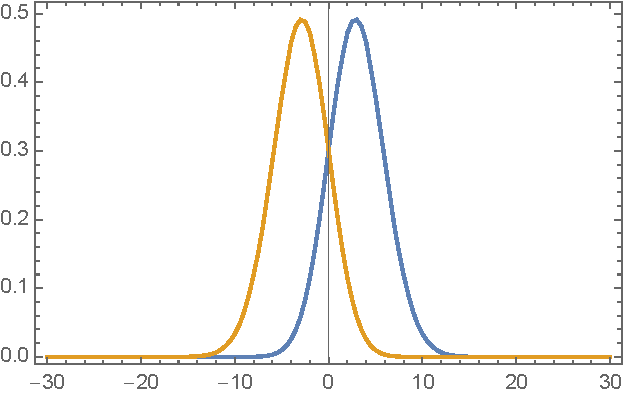
\includegraphics[width=\textwidth]{A4NumberDensity}
\caption{The swallowtail number density $\mathcal{N}(A_4^i)$ corresponding to the first and the second eigenvalue field. The swallowtail caustics corresponding to the first eigenvalue field (blue) and the second eigenvalue field (yellow).}
\end{subfigure}
\begin{subfigure}[b]{0.49\textwidth}
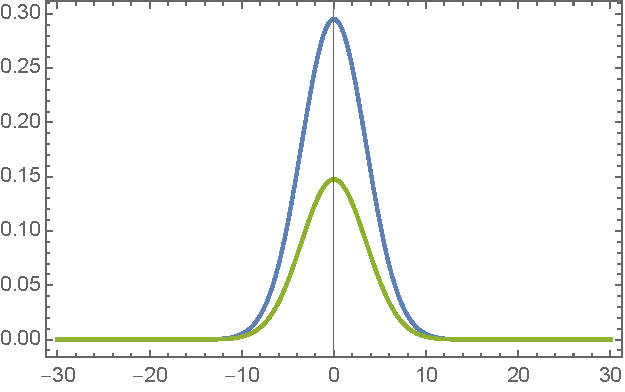
\includegraphics[width=\textwidth]{D4NumberDensity}
\caption{The number density $\mathcal{N}(D_4^{12-})$ and $\mathcal{N}(D_4^{12+})$ (blue), and $\mathcal{N}(D_4^{12\pm})$ (green) as a function of the eigenvalue $\lambda$.\\$ $\\}
\end{subfigure}
\caption{The number densities corresponding to the clusters in the caustic skeleton.}
\label{fig:clusternumberdensities}
\end{figure}


%%%%%%%%%%%%%%%%%%%%%%%%%%%%%%%%%%%%%%%%%%%%%%%%%%%%%%%%%%%%%%%%
\subsection{Numerical example}
We can study these statistics numerically for a realization of the density perturbation field. See figure \ref{fig:NumericalExample} for the caustic skeleton in Lagrangian space corresponding to the realization presented in figure \ref{fig:Example}. 

\begin{figure}
\centering
\begin{subfigure}[b]{0.49\textwidth}
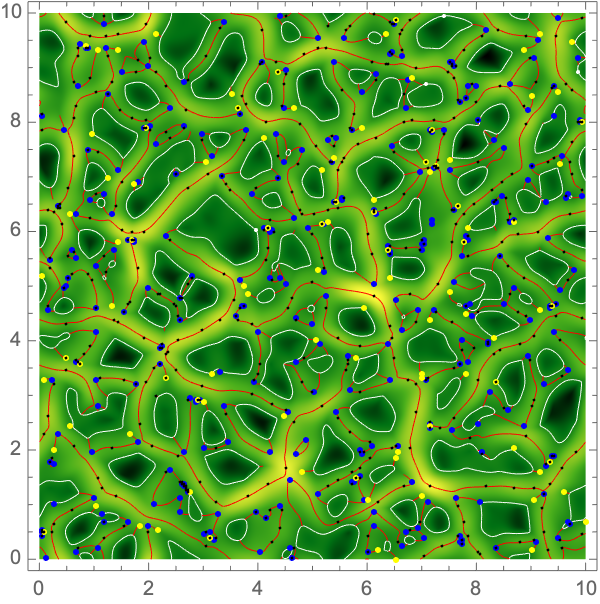
\includegraphics[width=\textwidth]{Lambda1}
\caption{The caustic skeleton corresponding to the first eigenvalue field $\lambda_1$}
\end{subfigure}
\begin{subfigure}[b]{0.49\textwidth}
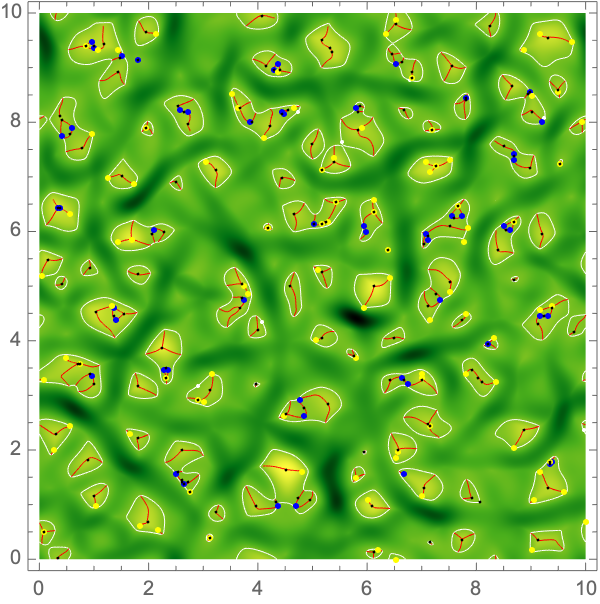
\includegraphics[width=\textwidth]{Lambda2}
\caption{The caustic skeleton corresponding to the second eigenvalue field $\lambda_2$}
\end{subfigure}
\caption{The caustic skeleton in Lagrangian space in a periodic $10\text{ Mpc } \times 10 \text{ Mpc}$ box with $2048 \times 2048$ grid points. The skeleton includes the shell-crossing curve $A_2^i$ corresponding to $b_+ \to \infty$ (white), the cusp curve $A_3^i$ (red), cusp points $A_3^{i\pm}$ (black), the swallowtail points $A_4^i$ (blue), and the umbilic points $D_4^{12}$.}
\label{fig:NumericalExample}
\vspace{1cm}
%\end{figure}
%
%\begin{figure}
%\centering
%\begin{subfigure}[b]{0.32\textwidth}
%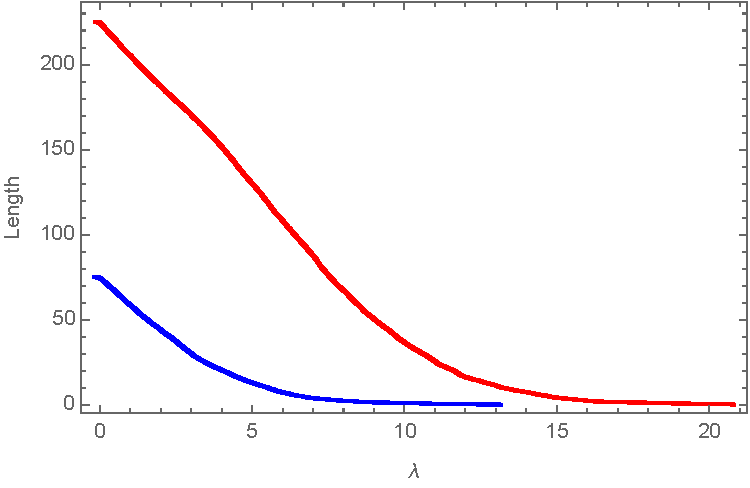
\includegraphics[width=\textwidth]{A3Length}
%\caption{The length of the $A_3$ lines as a function of the eigenvalue. The length $\mathcal{L}(A_3^1)$ in red and $\mathcal{L}(A_3^2)$ in blue.\\}
%\end{subfigure}
%\begin{subfigure}[b]{0.32\textwidth}
%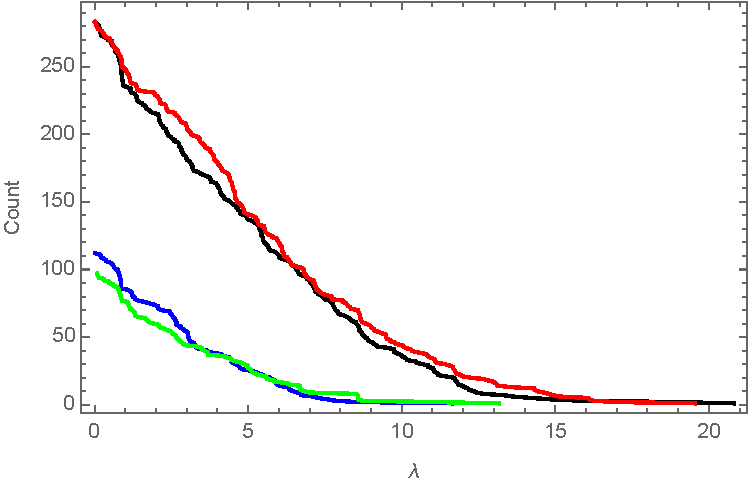
\includegraphics[width=\textwidth]{A3pm}
%\caption{The number of $A_3^{\pm}$ points as a function of the eigenvalue. The density of $A_3^{1+}$ (black), $A_3^{1-}$ (red), $A_3^{2+}$ (blue), and $A_3^{2-}$ (green) points.}
%\end{subfigure}
%\begin{subfigure}[b]{0.32\textwidth}
%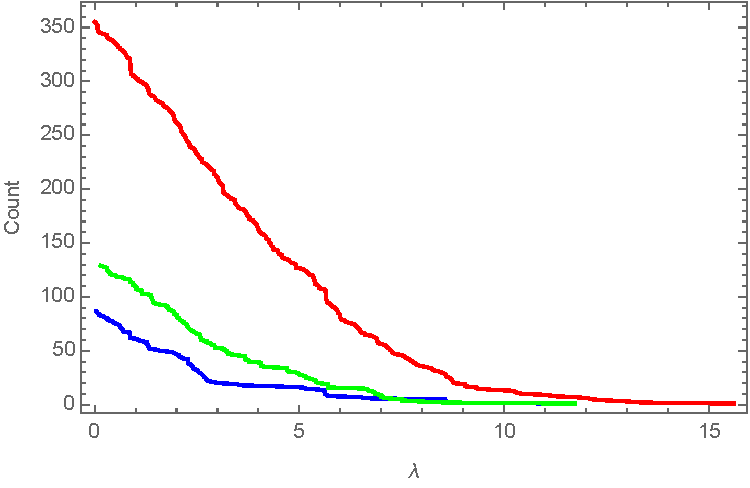
\includegraphics[width=\textwidth]{A4D4}
%\caption{The number of $A_4^1$ (red), $A_4^2$ (blue), and $D_4^{12}$ (green) points as a function of the eigenvalue.\\ $ $\\}
%\end{subfigure}
%\caption{The statistics of the caustic skeleton in Lagrangian space as a function of the eigenvalue field.}
%\label{fig:NumericalExampleStatistics}
\end{figure}


%%%%%%%%%%%%%%%%%%%%%%%%%%%%%%%%%%%%%%%%%%%%%%%%%%%%%%%%%%%%%%%%
\section{Constrained realizations}\label{sec:simulation}
Using the caustic conditions, we can find the statistical properties of patches of the initial conditions that lead to filaments and clusters.

%%%%%%%%%%%%%%%%%%%%%%%%%%%%%%%%%%%%%%%%%%%%%%%%%%%%%%%%%%%%%%%%
\subsection{Cusp caustics}
The cusp filaments are defined by the conditions $\lambda_i=\lambda$ and $\bm{v}_i \cdot \lambda_i = 0$. In the eigenframe, for the first eigenvalue field, this leads to the constraint manifold
\begin{align}
\mathcal{M}_{\mathcal{C}} = \{(T_{11},T_{12},T_{22}, T_{111})\,|\,   T_{11} = \lambda,T_{22}\leq \lambda,\text{ and }T_{12}=T_{111}=0\}\,.
\end{align}
We implement this condition in terms of the linear constraints
\begin{align}
C_1[\Psi;\bm{0}]=T_{11}\,,\quad
C_2[\Psi;\bm{0}]=T_{12}\,,\quad
C_3[\Psi;\bm{0}]=T_{22}\,,\quad
C_4[\Psi;\bm{0}]=T_{111}\,,
\end{align}
with $\bar{\bm{c}}=(\lambda,0,\bar{c}_3(\lambda),0)$. The average constraint $\bar{c}_3$ is given by the identity
\begin{align}
\bar{c}_3(\lambda) &= \int_{-\infty}^\lambda T_{22}\, p(T_{22}\,|\, T_{11}=\lambda, T_{12}=0,T_{111}=0)\mathrm{d}T_{22} \nonumber \\
&= \frac{\lambda}{3} + \tau_2^2 \frac{
 \text{Erfc}\left[\sqrt{\frac{2}{3}}\frac{\lambda}{\tau_2}\right]-2
 }{ \sqrt{\frac{6}{\pi}} \tau_2 e^{-\frac{2 \lambda^2}{3\tau_2^2}} -2 \lambda \left( \text{Erfc}\left[\sqrt{\frac{2}{3}}\frac{\lambda}{\tau_2}\right]-2 \right)}\,.
\end{align}
%See figure \ref{fig:A3_c2_constraint} for an illustration of the mean constraint $\bar{c}_3$.
%
%\begin{figure}
%\centering
%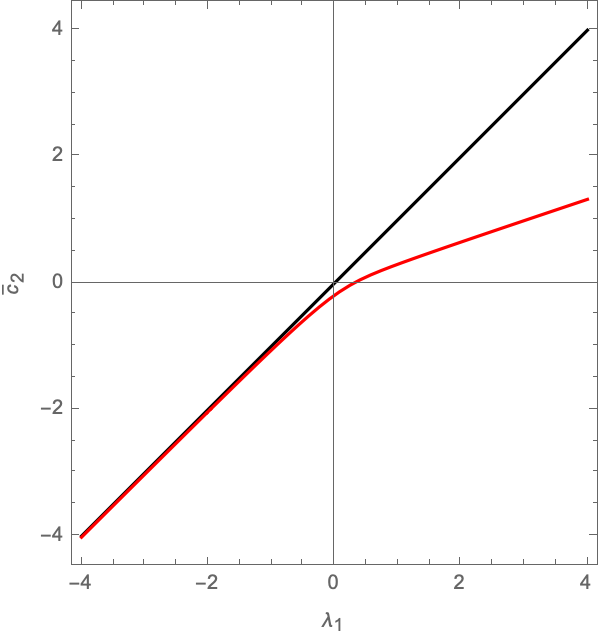
\includegraphics[width=0.45\textwidth]{A3_c2}
%\caption{The mean constraint $\bar{c}_2$ for the cusp filament for $\alpha =1$ and $R=1$.}
%\label{fig:A3_c2_constraint}
%\end{figure}


The mean displacement potential for the cusp filament  $\bar{\Psi}_{\bar{\bm{c}}}(\bm{q})$ in the initial conditions, for the power-law power spectrum smoothed by a Gaussian is given by
\begin{align}
\bar{\Psi}_{\bar{\bm{c}}}(\bm{q}) = 
-2 e^{-\frac{q^2}{8R^2}} R^2\left((\bar{c}_3(\lambda) + \lambda) I_{0}\left[\frac{q^2}{8R^2}\right]
+2 (\bar{c}_3(\lambda) - \lambda) I_{1}\left[\frac{q^2}{8R^2}\right] \cos (2\theta)\right)\,.
\end{align}
See figure \ref{fig:A3Mean} for an illustration of the mean field and the variance of the residue near the constraint.

\begin{figure}
\centering
\begin{subfigure}[b]{0.45\textwidth}
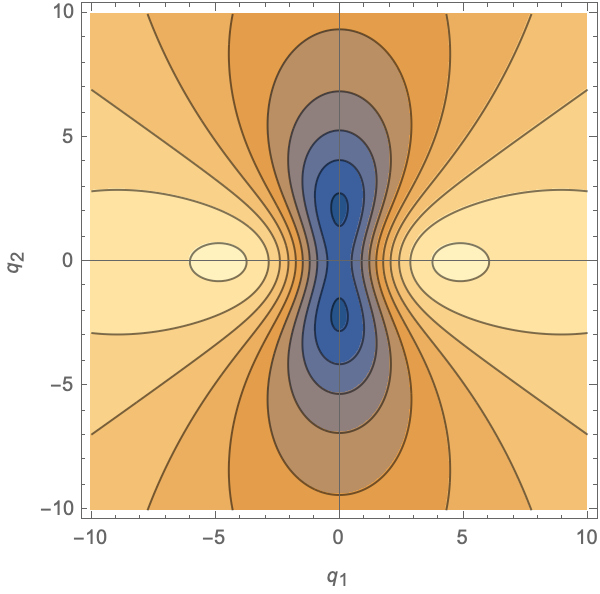
\includegraphics[width=\textwidth]{A3Mean_lambda=000}
\caption{Eigenvalue $\lambda=0$}
\end{subfigure}
\begin{subfigure}[b]{0.45\textwidth}
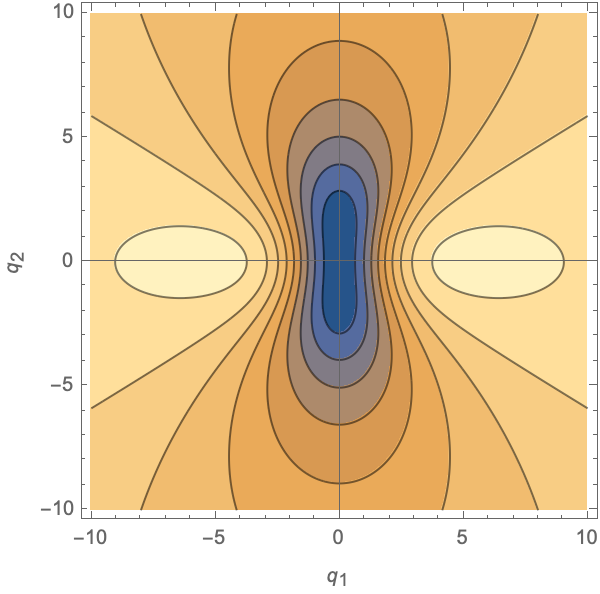
\includegraphics[width=\textwidth]{A3Mean_lambda=025}
\caption{Eigenvalue $\lambda=0.25$}
\end{subfigure}\\
\begin{subfigure}[b]{0.45\textwidth}
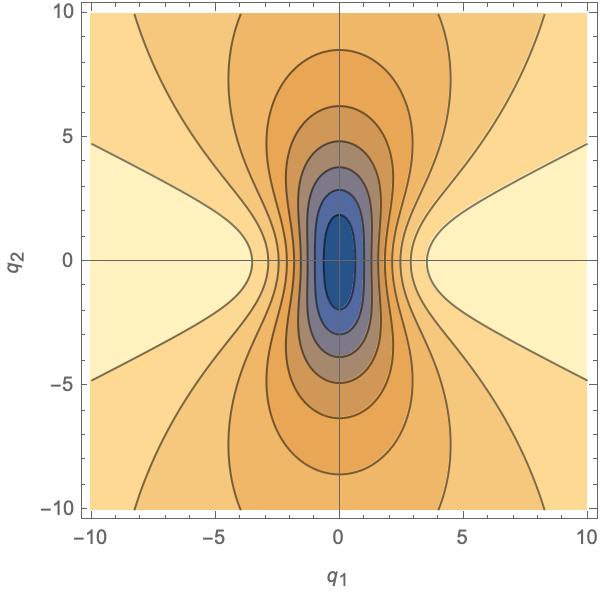
\includegraphics[width=\textwidth]{A3Mean_lambda=050}
\caption{Eigenvalue $\lambda=0.5$}
\end{subfigure}
\begin{subfigure}[b]{0.45\textwidth}
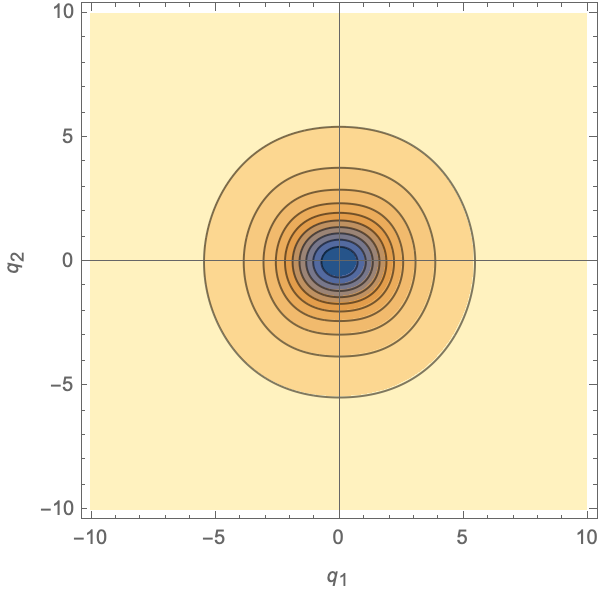
\includegraphics[width=\textwidth]{A3Variance}
\caption{Variance of the residue}
\end{subfigure}
\caption{The mean displacement potential for the cusp filament for $\alpha =1$ and $R=1$.}
\label{fig:A3Mean}
\end{figure}

%
%\begin{figure}
%\centering
%\begin{subfigure}[b]{0.45\textwidth}
%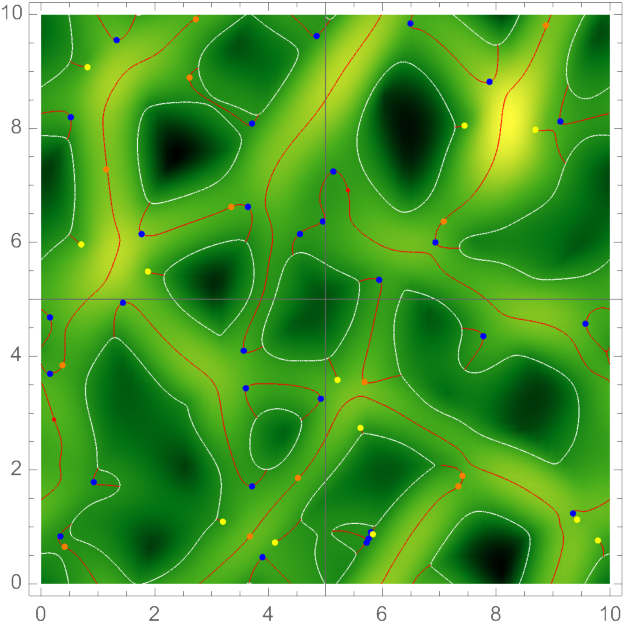
\includegraphics[width=\textwidth]{A3aGRF}
%\caption{Unstrained Gaussian random field}
%\label{fig:}
%\end{subfigure}
%\begin{subfigure}[b]{0.45\textwidth}
%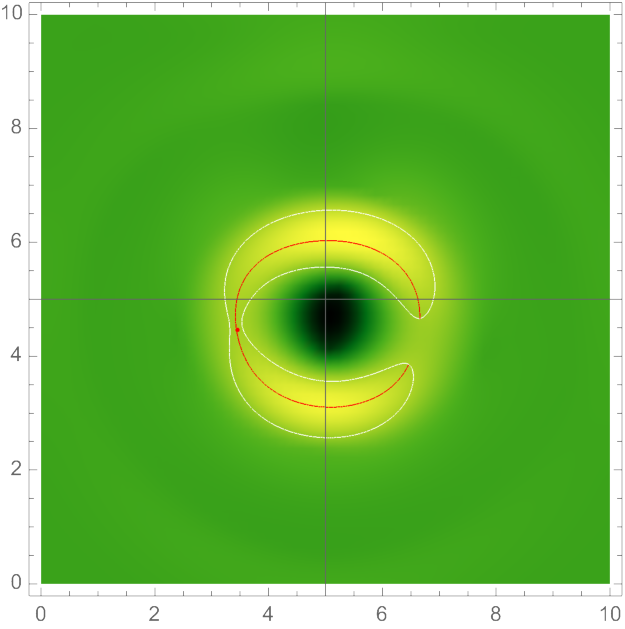
\includegraphics[width=\textwidth]{A3aFitField}
%\caption{Fit field corresponding to the GRF}
%\label{fig:}
%\end{subfigure}\\
%\begin{subfigure}[b]{0.45\textwidth}
%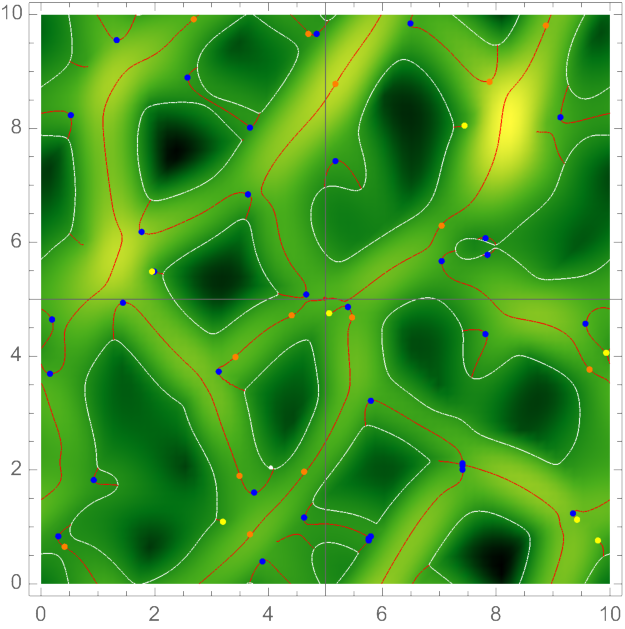
\includegraphics[width=\textwidth]{A3aCGRF}
%\caption{Constrained Gaussian random field}
%\label{fig:}
%\end{subfigure}
%\begin{subfigure}[b]{0.45\textwidth}
%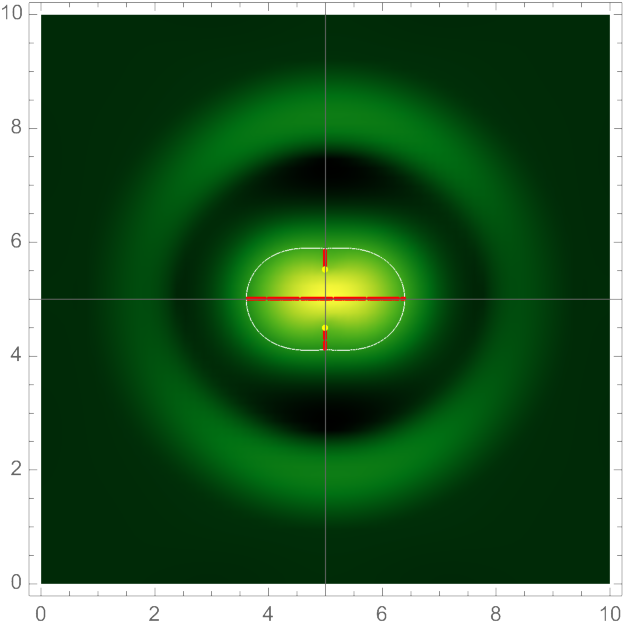
\includegraphics[width=\textwidth]{A3aMeanField}
%\caption{Mean field of the cusp filament}
%\label{fig:}
%\end{subfigure}
%\caption{$T_{11}=3, T_{22}=2,T_{12}=0$, and $T_{111}=0$.}
%\label{fig:}
%\end{figure}

The Morse-Smale points corresponding to the first eigenvalue field, $A_3^{1\pm}$, are, in the eigenframe, determined by constraint manifold
\begin{align}
\mathcal{M}_{\mathcal{C}} = \left\{(T_{11},T_{12},T_{22},T_{111},T_{112},T_{1111}) \,|\, T_{11}=\lambda, T_{12}=T_{111}=0,T_{1111}=-\frac{3T_{112}^2}{\lambda-T_{22}}\right\}\,.
\end{align}
We implement these conditions with the linear constraints
\begin{align}
C_1[\Psi;\bm{0}]&=T_{11}\,,\ \quad
C_2[\Psi;\bm{0}]=T_{12}\,,\ \quad
C_3[\Psi;\bm{0}]=T_{22}\,, \\
C_4[\Psi;\bm{0}]&=T_{111}\,,\quad
C_5[\Psi;\bm{0}]=T_{112}\,,\quad
C_6[\Psi;\bm{0}]=T_{1111}\,,
\end{align}
with the values $\bar{\bm{c}}=(\lambda, 0, \bar{c}_3(\lambda), 0, \bar{c}_5(\lambda),\bar{c}_6(\lambda))$, where
\begin{align}
\bar{c}_3(\lambda) &= \int_{\mathcal{M}_\mathcal{C}} T_{22}\,p(\bm{c}|\bm{c}\in \mathcal{M}_\mathcal{C})\mathrm{d}\bm{c}\,,\\
\bar{c}_5(\lambda) &= \int_{\mathcal{M}_\mathcal{C}} T_{112}\,p(\bm{c}|\bm{c}\in \mathcal{M}_\mathcal{C})\mathrm{d}\bm{c}\,,\\
\bar{c}_6(\lambda) &=-\frac{3\bar{c}_5(\lambda)^2}{\lambda-\bar{c}_3(\lambda)}\,.
\end{align}
The creation and merging points are selected by restricting the constraint manifold to the domain for which the determinant 
$\det\left(\nabla (\bm{v}_i \cdot \nabla \lambda_i), \nabla ((\nabla (\bm{v}_i \cdot \nabla \lambda_i))^\perp \cdot \nabla \lambda_i)\right)$ is either negative or positive.

%%%%%%%%%%%%%%%%%%%%%%%%%%%%%%%%%%%%%%%%%%%%%%%%%%%%%%%%%%%%%%%%
\subsection{Swallowtail caustics}
The swallowtail caustic is characterized by the conditions $\bm{v}_i \cdot \nabla \lambda_i=0$ and $\bm{v}_i \cdot \nabla (\bm{v}_i \cdot \nabla \lambda_i)=0$. This leads to very similar analysis as for the Morse points, where
\begin{align}
\bar{c}_3(\lambda)&= \int_{\mathcal{M}_\mathcal{C}} T_{22}\,p(\bm{c}\,|\,\bm{c}\in \mathcal{M}_\mathcal{C})\mathrm{d}\bm{c}\,,\\
\bar{c}_5(\lambda)&= \int_{\mathcal{M}_\mathcal{C}} T_{112}\,p(\bm{c}\,|\,\bm{c}\in \mathcal{M}_\mathcal{C})\mathrm{d}\bm{c}\,,\\
\bar{c}_6(\lambda)&= -\frac{3 \bar{c}_5^2}{\lambda - \bar{c}_3} \,.
\end{align}
The constraint $\bar{c}_5=0$ since $p(\bm{c}|\bm{c}\in \mathcal{M}_{\mathcal{C}})$ is symmetric under $T_{112}\to -T_{112}$. The constraint $\bar{c}_6$ vanishes since $\bar{c}_5$ does. 
%The constraint $\bar{c}_3$ is illustrated in figure \ref{fig:A4_c3_constraint}.

%\begin{figure}
%\centering
%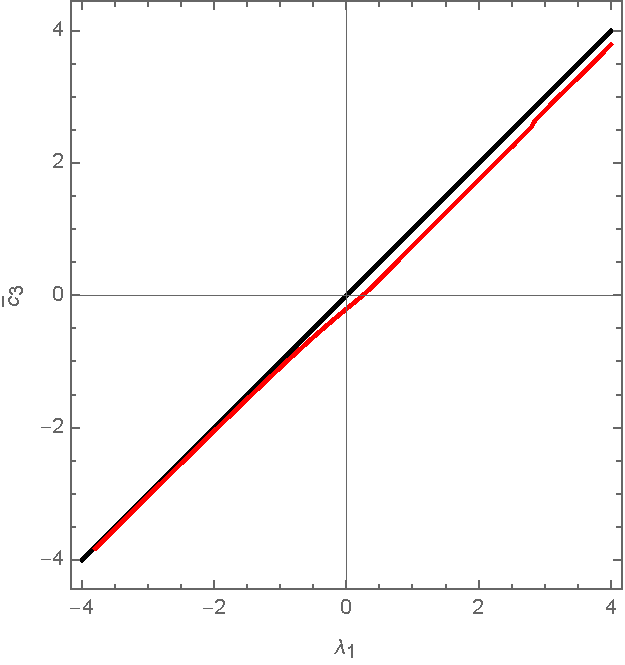
\includegraphics[width=0.45\textwidth]{A4_c3}
%\caption{The mean constraint $\bar{c}_3$ for the cusp filament for $\alpha =1$ and $R=1$.}
%\label{fig:A4_c3_constraint}
%\end{figure}

\begin{figure}
\centering
\begin{subfigure}[b]{0.45\textwidth}
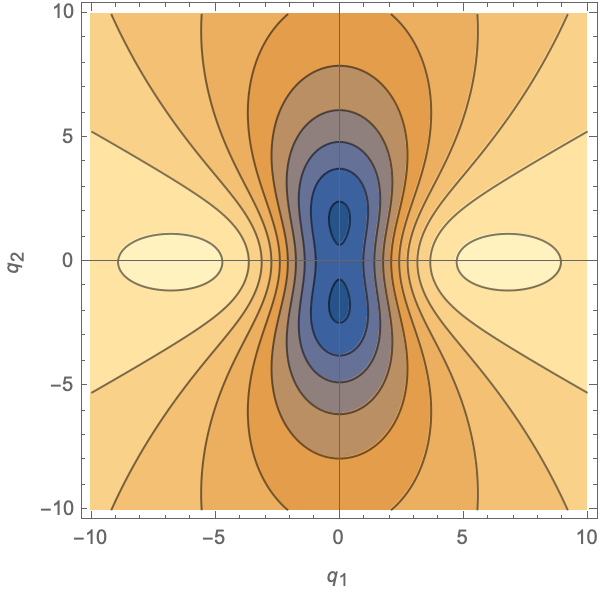
\includegraphics[width=\textwidth]{A4Mean_lambda=000}
\caption{Eigenvalue $\lambda=0$}
\end{subfigure}
\begin{subfigure}[b]{0.45\textwidth}
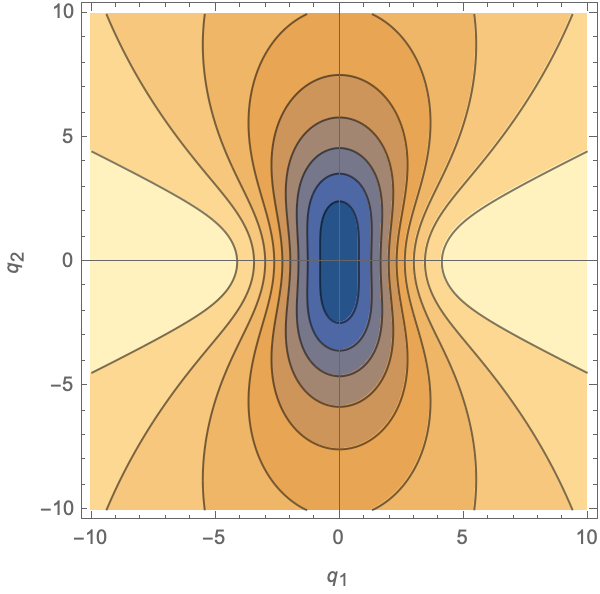
\includegraphics[width=\textwidth]{A4Mean_lambda=025}
\caption{Eigenvalue $\lambda=0.25$}
\end{subfigure}\\
\begin{subfigure}[b]{0.45\textwidth}
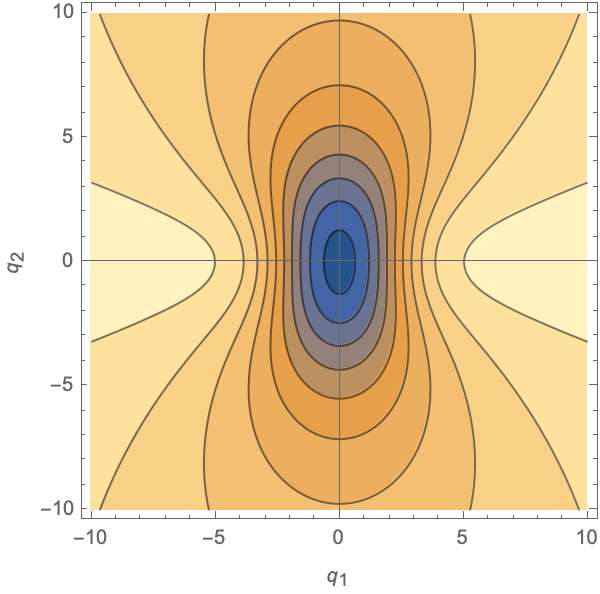
\includegraphics[width=\textwidth]{A4Mean_lambda=050}
\caption{Eigenvalue $\lambda=0.5$}
\end{subfigure}
\begin{subfigure}[b]{0.45\textwidth}
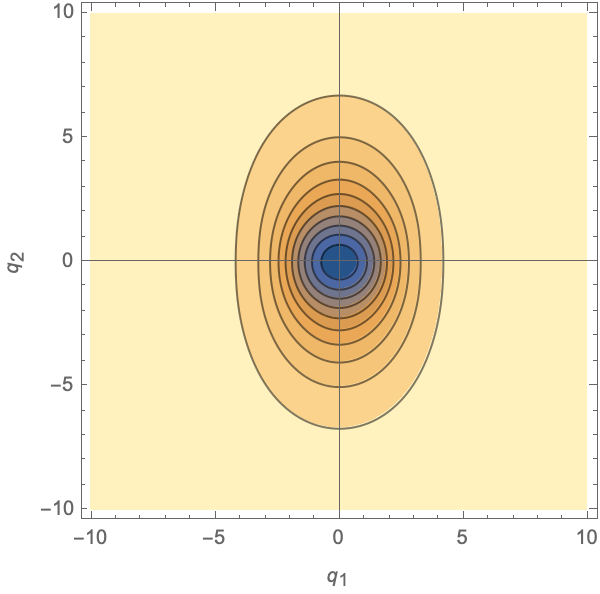
\includegraphics[width=\textwidth]{A4Variance}
\caption{Variance of the residue}
\end{subfigure}
\caption{The mean displacement potential for the swallowtail cluster for $\alpha =1$ and $R=1$.}
\label{fig:A4Mean}
\end{figure}

%%%%%%%%%%%%%%%%%%%%%%%%%%%%%%%%%%%%%%%%%%%%%%%%%%%%%%%%%%%%%%%%
\subsection{Umbilic caustics}
The umbilic caustics are defined by the linear conditions 
\begin{align}
C_1[\Psi;\bm{0}] = T_{11}\,,\quad
C_2[\Psi;\bm{0}] = T_{12}\,,\quad
C_3[\Psi;\bm{0}] = T_{22}\,.
\end{align}
with $\bm{c}=(\nu,\nu,0)$, which defines the constraint manifold 
\begin{align}
\mathcal{M}_{\mathcal{C}} = \{(T_{11},T_{12},T_{22})\,|\, T_{11}=T_{22} = \lambda, \text{ and } T_{12}=0\}\,,
\end{align}
consisting of a single point. For a random field with a power-law power spectrum with a Gaussian smoothing, the mean field
\begin{align}
\bar{\Psi}_{\mathcal{C}}(\bm{q}) =-4 e^{-\frac{q^2}{8R^2}}R^2 \lambda I_0\left[\frac{q^2}{8R^2}\right]\,,
\end{align}
with the modified Bessel function $I_0$, and $\bm{q}=(q\cos\theta, q\sin \theta)$. See \ref{fig:D4Mean} for an illustration. By specifying the third derivatives we can refine the mean field for the hyperbolic and elliptic umbilic points.



\begin{figure}
\centering
\begin{subfigure}[b]{0.45\textwidth}
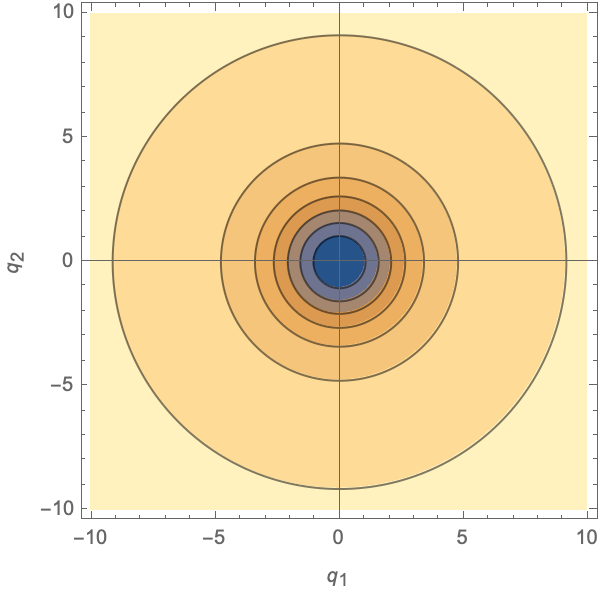
\includegraphics[width=\textwidth]{D4Mean}
\caption{Mean field}
\end{subfigure}
\begin{subfigure}[b]{0.45\textwidth}
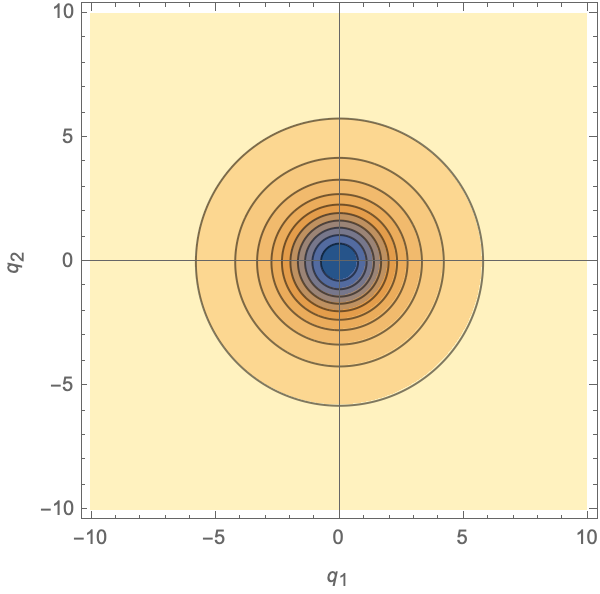
\includegraphics[width=\textwidth]{D4Variance}
\caption{Variance of the residue field}
\end{subfigure}
\caption{The mean displacement potential for the umbilic cluster for $\alpha =1$ and $R=1$.}
\label{fig:D4Mean}
\end{figure}




\begin{figure}
\vspace{-1.5cm}
\centering
\begin{subfigure}[b]{0.3\textwidth}
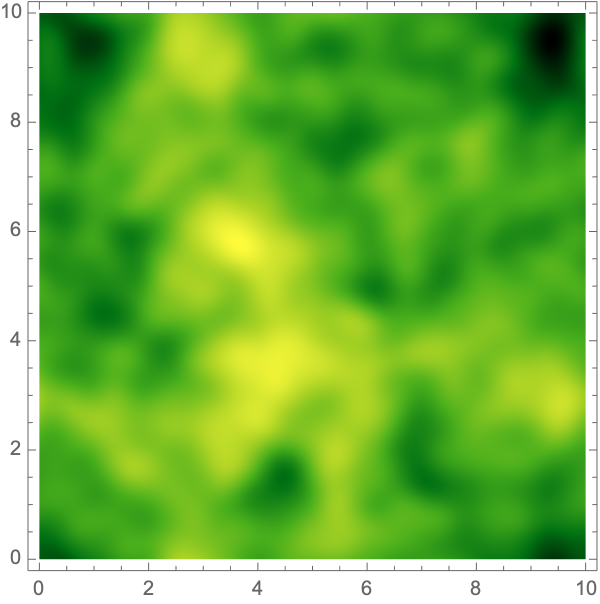
\includegraphics[width=\textwidth]{ScaleR=025_Psi}
\caption{$R=0.25\text{ Mpc}$}
\label{fig:}
\end{subfigure}
\begin{subfigure}[b]{0.3\textwidth}
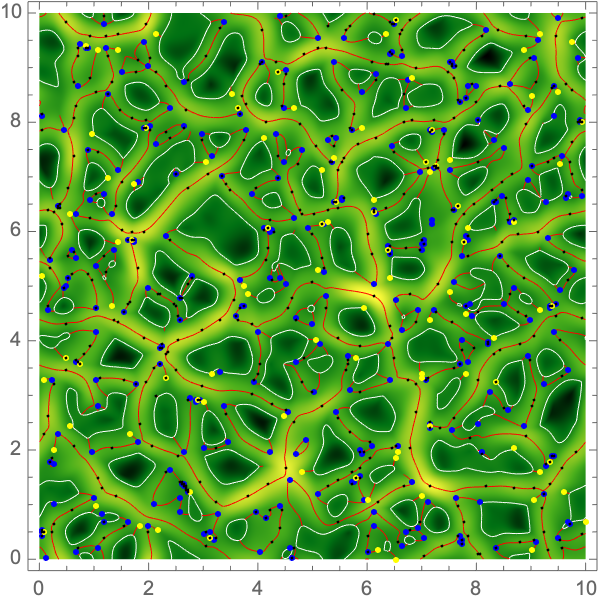
\includegraphics[width=\textwidth]{ScaleR=025_skelet}
\caption{$R=0.25\text{ Mpc}$}
\label{fig:}
\end{subfigure}
\begin{subfigure}[b]{0.3\textwidth}
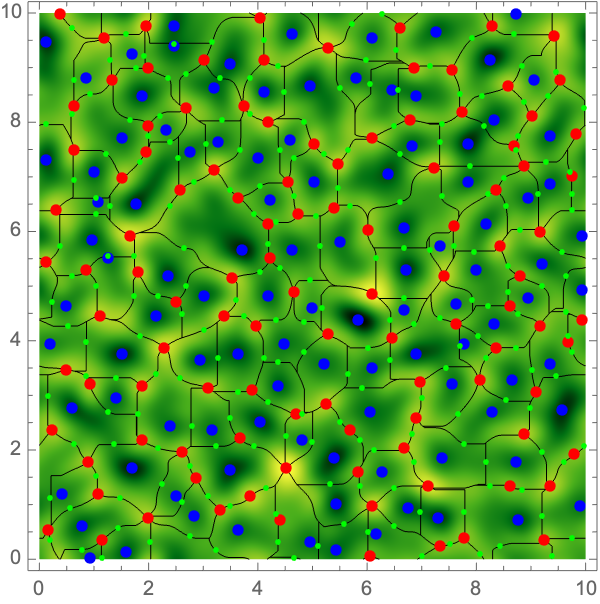
\includegraphics[width=\textwidth]{ScaleR=025_delta}
\caption{$R=0.25\text{ Mpc}$}
\label{fig:}
\end{subfigure}\\
\begin{subfigure}[b]{0.3\textwidth}
\includegraphics[width=\textwidth]{ScaleR=050_Psi}
\caption{$R=0.5\text{ Mpc}$}
\label{fig:}
\end{subfigure}
\begin{subfigure}[b]{0.3\textwidth}
\includegraphics[width=\textwidth]{ScaleR=050_skelet}
\caption{$R=0.5\text{ Mpc}$}
\label{fig:}
\end{subfigure}
\begin{subfigure}[b]{0.3\textwidth}
\includegraphics[width=\textwidth]{ScaleR=050_delta}
\caption{$R=0.5\text{ Mpc}$}
\label{fig:}
\end{subfigure}\\
\begin{subfigure}[b]{0.3\textwidth}
\includegraphics[width=\textwidth]{ScaleR=075_Psi}
\caption{$R=0.75\text{ Mpc}$}
\label{fig:}
\end{subfigure}
\begin{subfigure}[b]{0.3\textwidth}
\includegraphics[width=\textwidth]{ScaleR=075_skelet}
\caption{$R=0.75\text{ Mpc}$}
\label{fig:}
\end{subfigure}
\begin{subfigure}[b]{0.3\textwidth}
\includegraphics[width=\textwidth]{ScaleR=075_delta}
\caption{$R=0.75\text{ Mpc}$}
\label{fig:}
\end{subfigure}\\
\begin{subfigure}[b]{0.3\textwidth}
\includegraphics[width=\textwidth]{ScaleR=100_Psi}
\caption{$R=1\text{ Mpc}$}
\label{fig:}
\end{subfigure}
\begin{subfigure}[b]{0.3\textwidth}
\includegraphics[width=\textwidth]{ScaleR=100_skelet}
\caption{$R=1\text{ Mpc}$}
\label{fig:}
\end{subfigure}
\begin{subfigure}[b]{0.3\textwidth}
\includegraphics[width=\textwidth]{ScaleR=100_delta}
\caption{$R=1\text{ Mpc}$}
\label{fig:}
\end{subfigure}
\caption{The displacement potential, the caustic skeleton and the Morse-Smale complex on the density perturbations in scale space on in a $10\text{ Mpc}\times 10 \text{ Mpc}$ box with $2048 \times 2048$ grid points. The displacement potential (left), the caustic skeleton corresponding to the first eigenvalue field (centre), and the Morse-Smale skeleton corresponding to the density perturbation (right).}
\label{fig:ScaleSpace}
\vspace{-1.25cm}
\end{figure}

%%%%%%%%%%%%%%%%%%%%%%%%%%%%%%%%%%%%%%%%%%%%%%%%%%%%%%%%%%%%%%%%
\section{Scale space and Morse-Smale theory}\label{sec:ScaleSpace}
The hierarchical nature of the large scale structure is best captured by the properties of the cosmic web in scale space. In the right panels of figure \ref{fig:ScaleSpace}, we plot the displacement potential $\Psi$ corresponding to the power law $P(k) = k^{-2}$, in a periodic $10 \text{ Mpc} \times 10 \text{ Mpc}$ box with $2048^2$ lattice points, smoothed on different length scales $R=0.25,0.5,0.75$, and $1\text{ Mpc}$ with a Gaussian window function. Observe that smoothing at large length scales removes many of the fine details of the displacement potential. The same behaviour can be observed in the corresponding density perturbation field $\delta$ (the right panels of figure \ref{fig:ScaleSpace}) and the first eigenvalue field $\lambda_1$ (the central panels of figure \ref{fig:ScaleSpace}). Note that while the density perturbation corresponding to the smoothed displacement potential coincides with the smoothed density perturbation, this is not true for the eigenvalue fields due to the non-linear relations.

%%%%%%%%%%%%%%%%%%%%%%%%%%%%%%%%%%%%%%%%%%%%%%%%%%%%%%%%%%%%%%%%
\subsection{The caustic skeleton in scale space}
The caustic skeleton corresponding to the smoothed displacement potentials give a clear view of the hierarchical nature of the cosmic web. The skeleton at the scale $R=0.25$ is very fine and captures many of the features which evolve into tenuous structures. As we increase the length scale to $R=1$, the different cusp lines merge, anticipating the more global picture of the cosmic web. Note that by tracing the positions of the cusp points $A_3^\pm$ as a function of the scale $R$, we can trace the hierarchy nature of the filaments in the initial conditions. The quantitative properties of the caustic skeleton in scale space will be studied in an future publication [].


Following work by [When do cosmic peaks, filaments or walls merge? Cadiou et al. 2020], we can compute the number density of critical events of the eigenvalue fields by requiring that both the gradient vanishes and the Hessian is singular. That is to say, both the gradient
\begin{align}
\nabla \lambda_i = \bm{0}\,,
\end{align}
and the determinant of the Hessian vanishes
\begin{align}
\bm{H} &\equiv\mathcal{H}\lambda_i\,,\\
H &\equiv \det (\bm{H})\nonumber\\
&= \partial_1 \partial_1 \lambda_i\, \partial_2\partial_2 \lambda_i - (\partial_1 \partial_2 \lambda_i)^2\nonumber\\
&=0\,,
\end{align}
in the scale-space. The number density of critical events is given by
\begin{align}
\mathcal{N}_{ce} = 
\left\langle \left|J\right| \,
\delta_D^{(1)}(\lambda_i-\lambda)\,
\delta_D^{(2)}(\nabla \lambda_i)\,
\delta_D^{(1)}(H)
\right\rangle\,,
\end{align}
with the Jacobian 
\begin{align}
J &= \det 
\begin{pmatrix} 
\partial_R H 					& \nabla H \\
\partial_R \nabla \lambda_i  	& \bm{H}
\end{pmatrix}\nonumber\\
&= H(\partial_R H -\partial_R \nabla \lambda_i \cdot \bm{H}^{-1} \cdot \nabla H)\\
&= H \partial_R H
-\partial_R \partial_1 \lambda_i( 
\partial_1 H \, \partial_2 \partial_2 \lambda_i - \partial_2 H \, \partial_1 \partial_2\lambda_i    ) 
+ 
\partial_R \partial_2 \lambda_i (
 \partial_1 H \, \partial_1 \partial_2 \lambda_i 
 -
\partial_2  H \, \partial_1 \partial_1 \lambda_i )\,.\nonumber
\end{align}
Note that $H$ vanishes and $\bm{H}$ is singular at the critical events. As a consequence $H\partial_R H$ does not contribute to the expectation value and $\bm{H}^{-1}$ only makes sense in terms of the product $H \bm{H}^{-1}$. 

When scale-space is defined in terms of a Gaussian smoothing, we can use the identity
\begin{align}
\partial_R \Psi = R \nabla^2 \Psi\,,
\end{align}
to express the partial derivative of the eigenvalue fields with respect to the smoothing scale in terms of the derivatives of the displacement potential, \textit{i.e.},
\begin{align}
\partial_R \lambda_{1,2} = \frac{R}{2}\left[ \nabla^2 T_{11} + \nabla^2 T_{22} \pm \frac{4 T_{12} \nabla^2 T_{12} + (T_{11} - T_{22})(\nabla^2T_{11} - \nabla^2 T_{22})}{\sqrt{4T_{12}^2 + (T_{11}-T_{22})^2}}\right]\,.
\end{align}
The density $\mathcal{N}_{ce}$ counts both the merging and creation rate. We can distinguish between them by either integrating over positive or negative Jacobians, \textit{i.e.}
\begin{align}
\mathcal{N}_{ce \pm } = 
\left\langle \left|J\right| \,
\Theta_H(\pm J)\,
\delta_D^{(1)}(\lambda_i-\lambda)\,
 \delta_D^{(2)}(\nabla \lambda_i)\,
  \delta_D^{(1)}(H)
\right\rangle\,.
\end{align}

\begin{framed}
\noindent We should compare this with
\begin{align}
H &= \delta_{,11} \delta_{,22} - \delta_{,12}^2=0\,,
\end{align}
in the scale-space. The number density of critical events is given by
\begin{align}
\mathcal{N}_{ce} = 
\left\langle \left|J\right| \,
\delta_D^{(1)}(\delta-\lambda)\,
\delta_D^{(2)}(\nabla \delta )\,
\delta_D^{(1)}(H)
\right\rangle\,,
\end{align}
with the Jacobian 
\begin{align}
J 
&= H \partial_R H
-\partial_R \partial_1 \delta( 
\partial_1 H \, \delta_{,22} - \partial_2 H \, \delta_{,12}    ) 
+ 
\partial_R \partial_2 \delta (
 \partial_1 H \, \delta_{,12}
 -
\partial_2  H \,  \delta_{,11} )\\
&= H \partial_R H\\
&-R (\delta_{,112} + \delta_{,222})(2\delta_{,12}^2\delta_{,112} -3 \delta_{,11}\delta_{,22}\delta_{,112}-\delta_{,12}\delta_{,22}\delta_{,111} + \delta_{,11}^2 \delta_{,222})\\
&+R (\delta_{,111}+\delta_{,122})(2\delta_{,12}^2\delta_{,122} -3\delta_{,11} \delta_{,22}\delta_{,122}-\delta_{,11}\delta_{,12}\delta_{,222} + \delta_{,22}^2 \delta_{,111})\,.
\end{align}

We can simplify this calculation by inserting the identity
\begin{align}
\mathcal{I}(\delta_{,11},\delta_{,12},\delta_{,22}) = \pi (\delta_{,11}-\delta_{,22}) \Theta_H(\delta_{,11}-\delta_{,22})\delta_D^{(1)}(\delta_{,12})\,,
\end{align}
removing the integral over $\delta_{,12}$ and reducing the Jacobian to
\begin{align}
J 
&= H \partial_R H\\
&-R (\delta_{,112} + \delta_{,222})(-3 \delta_{,11}\delta_{,22}\delta_{,112} + \delta_{,11}^2 \delta_{,222})\\
&+R (\delta_{,111}+\delta_{,122})( -3\delta_{,11} \delta_{,22}\delta_{,122}+ \delta_{,22}^2 \delta_{,111})\,.
\end{align}
The integral over $\delta_{,11}$ reduces to the substitution $\delta_{,11}\to 0$ and the introduction of $\frac{1}{|\delta_{,22}|}$ since 
\begin{align}
\delta_D^{(1)}(\delta_{,11} \delta_{,22} - \delta_{,12}^2)\delta_D^{(1)}(\delta_{,12})=\frac{\delta_D^{(1)}(\delta_{,11})\delta_D^{(1)}(\delta_{,12})}{|\delta_{,22}|}\,.
\end{align}
This reduces the integral further to
\begin{align}
\mathcal{N}_{ce} &= 
\int \left|-R\delta_{,22}^2\delta_{,111}(\delta_{,111}+\delta_{,122})\right| \, \pi\, \\
&\times p(\delta,\delta_{,1}=0,\delta_{,2}=0,\delta_{,11}=0,\delta_{,12}=0,\delta_{,22},\delta_{,111},\delta_{,122})
\mathrm{d}\delta_{,22}\mathrm{d}\delta_{,111}\mathrm{d}\delta_{,122}\,.
\end{align}
integrated over $\delta_{,22}\leq 0$ since $-\delta_{,22}/|\delta_{,22}| = 1$.
\end{framed}

%%%%%%%%%%%%%%%%%%%%%%%%%%%%%%%%%%%%%%%%%%%%%%%%%%%%%%%%%%%%%%%%
\subsection{The Morse-Smale complex}
In the right panels of figure \ref{fig:ScaleSpace}, we plot the critical points of the density perturbation $\delta$ and the corresponding integral lines between the saddle points to the maxima. These integral lines separated the unstable manifolds of the minima of the field. It is often assumed that this tessellation of Lagrangian space gives an insightful picture of the seeds of the cosmic web, since the maxima and the integral lines between the saddle points and the maxima will tend to form clusters and filaments in the gravitational collapse. The minima of the density perturbation are often assumed to form void regions.

The comparison between the Morse-Smale complex of the density perturbation and the caustic skeleton of the deformation tensor is striking. The two skeletons agree on the global properties of the large-scale structure but differ in detail. The caustic skeleton shows a number of filaments and clusters that are not captured by the Morse-Smale analysis. Note that while the correspondence between the Morse-Smale skeleton is ad hoc, the caustic skeleton is directly related to the multi-stream nature of Lagrangian fluid dynamics (and the Zel'dovich approximation in particular).

The geometric differences of the two skeletons can be understood in terms of their algebraic definitions. While the critical points in the Morse-Smale skeleton are locally defined in the density perturbation field, the caustic skeleton obeys non-local and non-linear relations, relying on the gravitational potential corresponding to the density perturbation and the non-linear nature of the eigenvalue and eigenvector fields. We expect the differences to become enhanced for three-dimensional large scale structure formation. While the two-dimensional eigenvalue fields are roots of a quadratic equation, the three-dimensional eigenvalue fields are roots of a cubic equation.

At first sight, the Morse-Smale skeleton might seem computationally simpler than the caustic skeleton. This is certainly true for the clusters. However, this is not the case for the filaments and walls in the three-dimensional extension. While the filaments of the caustic skeleton are defined by a non-linear local equation in terms of the displacement potential, allowing for a fast evaluation and a detailed statistical analysis provided in this paper, the definition of the filaments in the Morse-Smale skeleton is non-local. In order for a point to be part of an integral line, we need to verify that the point flows from a saddle point to a maximum. The analysis of the filaments in the Morse-Smale skeleton, for this reason, always relies on a number of [stiff] approximations.


%%%%%%%%%%%%%%%%%%%%%%%%%%%%%%%%%%%%%%%%%%%%%%%%%%%%%%%%%%%%%%%%
\section{The late time cosmic web}
We so far studied the caustic skeleton in Lagrangian space. In order to model the formation of the filaments and clusters of the cosmic web, we push skeleton to Eulerian space with the Lagrangian map $\bm{x}_t$. We will here consider the Zel'dovich approximation
\begin{align}
\bm{x}_t(\bm{q}) =\bm{q}-b_+(t)\nabla \Psi(\bm{q})\,,
\end{align}
where the mass elements follow a ballistic trajectory, the \textit{scotch flow} where the mass elements follow the Zel'dovich approximation till shell-crossing where they freeze
\begin{align}
\bm{x}_t(\bm{q})=\bm{q}-\frac{1}{\lambda_i}\nabla\Psi(\bm{q})\,,
\end{align}
and an $N$-body simulation capturing the full non-linear evolution. 

See figure \ref{fig:EulerianSkeletonSimulation} for a visual comparison of the three skeletons in Eulerian space. We observe that skeleton corresponding to the Zel'dovich flow is accurate till the gravitational interaction turns the mass elements around. At late times, the skeleton does no longer resemble the cosmic structure. On the other hand, the skeleton corresponding to the $N$-body simulation captures the full geometry of the web demonstrating the power of the caustic skeleton. Unfortunately, we cannot use the $N$-body flow to analytically predict the statistical properties of the cosmic web. The scotch flow is an intermediate solution, which is analytically traceable and is an accurate approximation when the mass elements turn around and the Zel'dovich flow starts to fail. Note that more advanced analytic approximations of the Lagrangian fluid may lead to an even better analytic prediction of the cosmic structure.

\begin{figure}
\centering
\begin{subfigure}[b]{0.32\textwidth}
\includegraphics[width=\textwidth]{Visual_Zeldovich_D=1}
\caption{The Zel'dovich flow $b_+=1$}
\end{subfigure}
\begin{subfigure}[b]{0.32\textwidth}
\includegraphics[width=\textwidth]{Visual_Scotch_D=1}
\caption{The scotch flow $b_+=1$}
\end{subfigure}
\begin{subfigure}[b]{0.32\textwidth}
\includegraphics[width=\textwidth]{Visual_Nbody_D=1}
\caption{The $N$-body flow $b_+=1$}
\end{subfigure}\\
\begin{subfigure}[b]{0.32\textwidth}
\includegraphics[width=\textwidth]{Visual_Zeldovich_D=2}
\caption{The Zel'dovich flow $b_+=2$}
\end{subfigure}
\begin{subfigure}[b]{0.32\textwidth}
\includegraphics[width=\textwidth]{Visual_Scotch_D=2}
\caption{The scotch flow $b_+=2$}
\end{subfigure}
\begin{subfigure}[b]{0.32\textwidth}
\includegraphics[width=\textwidth]{Visual_Nbody_D=2}
\caption{The $N$-body flow $b_+=2$}
\end{subfigure}
\caption{The caustic skeleton in Eulerian space for growing mode $b_+=1$ and $b_+=2$ corresponding to the initial conditions shown in figure \ref{fig:visualization}. The caustics of the Zel'dovich approximation are pushed forward with the Zel'dovich approximation (left panels), the scotch flow (central panels), and a dark matter $N$-body simulation. The background of the left panels are virtualisations of the Zel'dovich approximation. The background in the central and right panels are visualizations of the $N$-body simulation.}
\label{fig:EulerianSkeletonSimulation}
\end{figure}

To derive the statistics of the cusp curve in Eulerian space, consider an infinitesimal line element $(\bm{q}, \bm{q}+\Delta\bm{q})$ in Lagrangian space, which mapped to the line element $(\bm{x}_t(\bm{q}), \bm{x}_t(\bm{q} + \Delta \bm{q}))$ in Eulerian space. The distance of these points is given by $\|\bm{x}_t(\bm{q}) - \bm{x}_t(\bm{q} + \Delta \bm{q})\| = \| \nabla_{\bm{q}}\bm{x}_t \Delta \bm{q}\|$ with the deformation tensor $\nabla_{\bm{q}}\bm{x}_t $. It follows, that the line length density of the cusp curves in Eulerian space takes the form
\begin{align}
\mathcal{L}_{\mathcal{E}}(A_3^i)&=
\langle \| \nabla_{\bm{q}}\bm{x}_t \nabla (\bm{v}_i \cdot \nabla \lambda_i)\|\, \delta_D^{(1)}(\lambda_i - \lambda)\,
\delta_D^{(1)}(\bm{v}_i\cdot \nabla \lambda_i)\rangle\,.
\end{align}
For the Zel'dovich approximation, the deformation tensor in the eigenframe
\begin{align}
\nabla_{\bm{q}}\bm{x}_t(\bm{q})=  \begin{pmatrix}1-b_+(t)\lambda_1(\bm{q}) & 0 \\ 0 &1-b_+(t) \lambda_2(\bm{q})\end{pmatrix}\,.
\end{align}
leads to the expectation value
\begin{align}
\mathcal{L}_{\mathcal{E}}(A_3^i)=&\,
\big \langle \sqrt{
((1-b_+(t)\lambda_1) \bm{v}_1 \cdot \nabla (\bm{v}_i \cdot \nabla \lambda_i))^2+
((1-b_+(t)\lambda_2) \bm{v}_2 \cdot \nabla (\bm{v}_i \cdot \nabla \lambda_i))^2
}\nonumber\\
&\times \delta_D^{(1)}(\lambda_i - \lambda)\,
\delta_D^{(1)}(\bm{v}_i\cdot \nabla \lambda_i)\big\rangle\,.
\end{align}

Under the Scotch flow, the deformation tensor takes the form
\begin{align}
\nabla_{\bm{q}}\bm{x}_t(\bm{q}) =I  - \frac{\bm{\psi}}{\lambda_i}  + \frac{\nabla_{\bm{q}} \lambda_i(\bm{q}) \nabla_{\bm{q}}\Psi}{\lambda_i(\bm{q})^2} \,,
\end{align}
which in the eigenframe yields
\begin{align}
\nabla_{\bm{q}}\bm{x}_t(\bm{q})
= 
\begin{pmatrix}
1 - \frac{\lambda_1}{\lambda_i} + \frac{(\bm{v}_1 \cdot \nabla \lambda_i) (\bm{v}_1 \cdot \nabla \Psi)}{\lambda_i^2} & \frac{(\bm{v}_2 \cdot \nabla \lambda_i) (\bm{v}_1 \cdot \nabla \Psi)}{\lambda_i^2} \\
\frac{(\bm{v}_1 \cdot \nabla \lambda_i) (\bm{v}_2 \cdot \nabla \Psi)}{\lambda_i^2} & 
1 - \frac{\lambda_2}{\lambda_i} + \frac{(\bm{v}_2 \cdot \nabla \lambda_i) (\bm{v}_2 \cdot \nabla \Psi)}{\lambda_i^2}
\end{pmatrix}.
\end{align}
The corresponding line length density $\mathcal{L}_{\mathcal{E}}$ is now an local expectation value in terms of the derivatives of the displacement potential at a single point. The correlation functions of the various points in the skeleton can be evaluated in a similar fashion.





%%%%%%%%%%%%%%%%%%%%%%%%%%%%%%%%%%%%%%%%%%%%%%%%%%%%%%%%%%%%%%%%
\section{Conclusion}\label{sec:conclusion}


%%%%%%%%%%%%%%%%%%%%%%%%%%%%%%%%%%%%%%%%%%%%%%%%%%%%%%%%%%%%%%%%
\section*{Acknowledgements}
We are most grateful to Johan Hidding, Bernard Jones and Neil Turok for many useful and encouraging discussions. JF acknowledges the Perimeter Institute for facilitating this research through the support by the Government of Canada through the Department of Innovation, Science and Economic Development Canada and by the Province of Ontario through the Ministry of Research, Innovation, and Science.

%\bibliographystyle{JHEP}
\bibliographystyle{plain}

\bibliography{mybibliography}

%%%%%%%%%%%%%%%%%%%%%%%%%%%%%%%%%%%%%%%%%%%%%%%%%%%%%%%%%%%%%%%%
\appendix

%%%%%%%%%%%%%%%%%%%%%%%%%%%%%%%%%%%%%%%%%%%%%%%%%%%%%%%%%%%%%%%%
\section{Gaussian random fields algorithms}\label{ap:GRF}
Realizations of Gaussian random fields on rectangular lattices can be generated using Fast Fourier Transforms using the property that the Fourier modes of a realization are samples from independent Gaussian distributions. The standard deviation of Gaussian distribution is given by the square root of the power spectrum. In this paper we use the following algorithm.\\


\begin{algorithm}[H]
\SetAlgoLined
\begin{enumerate}[itemsep=1ex, leftmargin=0cm, rightmargin=1cm]
\item Generate a realization of white noise $n_w(\bm{q})$, consisting of identically independently distributed normal numbers $\mathcal{N}(\mu=0,\sigma^2=1)$.
\item Fast Fourier transform the white noise $\hat{n}_w(\bm{k}) = \text{FFT}[n_w(\bm{q})]$. These modes are independently normally distributed with the reality condition $\hat{n}_w(\bm{k}) = \hat{n}_w^*(-\bm{k})$.
\item Rescale the Fourier modes with the power spectrum $\hat{f}(\bm{k}) = \sqrt{P(\bm{k})}\hat{n}_w(\bm{k})$.
\item Inverse fast Fourier transform the rescaled modes to obtain the realization of the unconstrained Gaussian random field $f(\bm{q}) = \text{FFT}^{-1}[\hat{f}(\bm{k})]$.
\end{enumerate}
 \caption{Generating a realization of an unconstrained Gaussian random field on a rectangular lattice}
 \label{alg:GRF}
\end{algorithm}$ $\\


Constrained Gaussian random fields are a bit more difficult to generate since the residue of the field is not stationary. In this paper, we make use of the Hoffman Ribak algorithm, leveraging the fact that the residue of a constrained Gaussian random field is independent of the value of the constraints.\\

\begin{algorithm}[H]
\SetAlgoLined
\begin{enumerate}[itemsep=1ex, leftmargin=0cm, rightmargin=1cm]
\item Generate a realization of an unconstrained Gaussian random field $g$ with the required power spectrum using algorithm \ref{alg:GRF}.
\item Evaluate the linear constraints $C_i$ of the unconstrained field $g$,
\begin{align}
d_i = C_i[g;\bm{q}_i]\,.
\end{align} 
\item Evaluate the mean field corresponding to the constraint values $d_i$,
\begin{align}
\bar{g}(\bm{q}) = \sum_{ij}\xi_i(\bm{q}) \xi^{-1}_{ij} d_j\,.
\end{align}
\item Evaluate the residue of the unconstrained field 
\begin{align}
G=g - \bar{g}\,.
\end{align}
\item Since the residue $G$ is statistically independent of the values $d_j$, we can identify $G$ with the residue $F$ of the constrained random field. The realization of the constrained Gaussian random field takes the form
\begin{align}
f(\bm{q}) = \sum_{ij}\xi_i(\bm{q}) \xi^{-1}_{ij} c_j + G(\bm{q})\,.
\end{align}
\end{enumerate}
 \caption{The Hoffman-Ribak method for Gaussian random fields with linear constraints}
 \label{alg:HoffmanRibak}
\end{algorithm}


%%%%%%%%%%%%%%%%%%%%%%%%%%%%%%%%%%%%%%%%%%%%%%%%%%%%%%%%%%%%%%%%
\section{Correlation functions of the derivatives of a Gaussian random field}\label{ap:correlations}

We here give explicit expressions for the local and the non-local correlations functions used in this paper.

%%%%%%%%%%%%%%%%%%%%%%%%%%%%%%%%%%%%%%%%%%%%%%%%%%%%%%%%%%%%%%%%
\subsection{Local correlation functions}
When evaluating the correlations between derivatives at a single points, we obtain
\begin{align}
\left\langle \frac{\partial^{n_1+m_1}\Psi(\bm{0})}{\partial q_1^{n_1}\partial q_2^{m_1}} \frac{\partial^{n_2+m_2}\Psi(\bm{0})}{\partial q_1^{n_2}\partial q_2^{m_2}}\right\rangle =&\,
\frac{1}{(2\pi)^4} \int  \langle \hat{\Psi}(\bm{k}_1)\hat{\Psi}^*(\bm{k}_2)\rangle (-i k_{1,1})^{n_1} (-i k_{1,2})^{m_1}\\
&\times(i k_{2,1})^{n_2} (i k_{2,2})^{m_2} \mathrm{d}\bm{k}_1 \mathrm{d}\bm{k}_2\nonumber\\
=&\,\frac{(-1)^{n_1+m_1}i^{n_1+m_1+n_2+m_2}}{(2\pi)^2} \int  P_\Psi(k)  k_{1}^{n_1+n_2}  k_{2}^{m_1+m_2} \mathrm{d}\bm{k}\nonumber\\
=&\,\frac{(-1)^{n_1+m_1}i^{n_1+m_1+n_2+m_2}}{(2\pi)^2} \int_0^\infty  P_\Psi(k)  k^{n_1+n_2+m_1+m_2} \mathrm{d} k\nonumber\\
&\,\times \int_0^{2\pi} \cos(\theta)^{n_1+n_2} \sin(\theta)^{m_1+m_2}\mathrm{d}\theta\nonumber\\
=&\,\frac{(-1)^{n_1+m_1}i^{n_1+m_1+n_2+m_2}}{2\pi} \tau^2_{\frac{1}{2}(n_1+n_2+m_1+n_2)}\nonumber\\
&\times \int_0^{2\pi} \cos(\theta)^{n_1+n_2} \sin(\theta)^{m_1+m_2}\mathrm{d}\theta\,.
\end{align}
Now note that
\begin{align}
\int_0^{2\pi} \cos(\theta)^{n_1+n_2} \sin(\theta)^{m_1+m_2}\mathrm{d}\theta = 0\,,
\end{align}
when $n_1+n_2$ or $m_1+m_2$ are odd. For even $n_1+n_2$ and $m_1+m_2$, the angular integral can be expressed in terms of the Gamma function
\begin{align}
\int_0^{2\pi} \cos(\theta)^{n_1+n_2} \sin(\theta)^{m_1+m_2}\mathrm{d}\theta = 
\frac{2 \Gamma\left(\frac{1}{2}(1+n_1+n_2)\right)\Gamma\left(\frac{1}{2}(1+m_1+m_2)\right)}{\Gamma\left(1+\frac{1}{2}(n_1+n_2+m_1+m_2)\right)}\,.
\end{align}
The local correlation is thus given by
\begin{align}
\left\langle \frac{\partial^{n_1+m_1}\Psi(\bm{0})}{\partial q_1^{n_1}\partial q_2^{m_1}} \frac{\partial^{n_2+m_2}\Psi(\bm{0})}{\partial q_1^{n_2}\partial q_2^{m_2}}\right\rangle 
=&\frac{(-1)^{n_1+m_1}i^{n_1+m_1+n_2+m_2}}{2\pi} \tau^2_{\frac{1}{2}(n_1+m_1+n_2+m_2)}\nonumber\\
&\times 
\frac{2 \Gamma\left(\frac{1}{2}(1+n_1+n_2)\right)\Gamma\left(\frac{1}{2}(1+m_1+m_2)\right)}{\Gamma\left(1+\frac{1}{2}(n_1+m_1+n_2+m_2)\right)}\,,
\end{align}
when $n_1+n_2$ and $m_1+m_2$ are even, and zero otherwise.

In this paper, we consider correlations of up to five derivatives. It follows from these relations that the distribution factorizes as follows
%\begin{align}
%p(&
%T;
%T_1,T_2;
%T_{11},T_{12},T_{22};
%T_{111},T_{112},T_{122},T_{222}; \nonumber\\
%&T_{1111},T_{1112},T_{1122},T_{1222},T_{2222};
%T_{11111},T_{11112},T_{11122},T_{11222},T_{12222},T_{22222})\nonumber\\
%=&\, p(T, T_{11},T_{22},T_{1111},T_{1122},T_{2222})
%\,\times p(T_{12},T_{1112}T_{1222})\nonumber\\
%&\,\times p(T_{1},T_{111},T_{122},T_{11111},T_{11122},T_{12222})\nonumber\\
%&\,\times p(T_2,T_{222},T_{112},T_{11112},T_{11222},T_{22222})
%\end{align}
\begin{align}
p(&
T;
T_1,T_2;
T_{11},T_{12},T_{22};
T_{111},T_{112},T_{122},T_{222}; 
T_{1111},T_{1112},T_{1122},T_{1222},T_{2222};
T_{11111},T_{22222})\nonumber\\
=&\, p(T, T_{11},T_{22},T_{1111},T_{1122},T_{2222})
\,\times p(T_{12},T_{1112}T_{1222})\nonumber\\
&\,\times p(T_{1},T_{111},T_{122},T_{11111})
\times p(T_2,T_{222},T_{112},T_{22222})
\end{align}
This is an useful property while evaluating the statistics of the caustic skeleton.

%%%%%%%%%%%%%%%%%%%%%%%%%%%%%%%%%%%%%%%%%%%%%%%%%%%%%%%%%%%%%%%%
\subsection{Non-local correlation functions}
For the correlation of the displacement potential and its derivatives at separate points, we obtain the relation
\begin{align}
\left\langle \Psi(\bm{q}) \frac{\partial^{n+m}\Psi(\bm{0})}{\partial q_1^n\partial q_2^m}\right\rangle &=
\frac{1}{(2\pi)^4} \int  \langle \hat{\Psi}(\bm{k}_1)\hat{\Psi}^*(\bm{k}_2)\rangle e^{-i \bm{k}_1 \cdot \bm{q}} (i k_{2,1})^n (i k_{2,2})^m \mathrm{d}\bm{k}_1 \mathrm{d}\bm{k}_2\nonumber\\
&=\frac{i^{n+m}}{(2\pi)^2} \int  P_\Psi(k) e^{-i \bm{k} \cdot \bm{q}} k_{1}^n  k_{2}^m \mathrm{d}\bm{k}\nonumber\\
&=\frac{i^{n+m}}{(2\pi)^2} \int_0^\infty  P_\Psi(k)  k^{n+m} \left[\int_0^{2\pi} e^{-i k q \cos(\alpha-\theta)} \cos^n \alpha \sin^m \alpha \mathrm{d}\alpha\right]\mathrm{d}k\,,
\end{align}
using the inner product $\bm{k}\cdot \bm{q}=k q \cos (\alpha-\theta)$ with $k=\|\bm{k}\|$ and $q=\|\bm{q}\|$. The integral over the angular variable can be expressed in terms of Bessel functions $J_n$. For the correlation of the displacement potential up to its fourth order derivative, we find the explicit expressions:
\begin{align}
\langle \Psi(\bm{q}) \Psi(\bm{0})\rangle &=\frac{1}{2\pi} \int_0^\infty P_{\Psi}(k) J_0(kq)\mathrm{d}k = \xi(q)\,,
\end{align}
the first derivative
\begin{align}
\langle \Psi(\bm{q}) T_1(\bm{0})\rangle &=\frac{\cos\theta}{2\pi} \int_0^\infty k P_{\Psi}(k) J_1(kq) \mathrm{d}k\,,\\
\langle \Psi(\bm{q}) T_2(\bm{0})\rangle &=\frac{\sin\theta}{2\pi} \int_0^\infty k P_{\Psi}(k) J_1(kq) \mathrm{d}k\,,
\end{align}
the second derivative
\begin{align}
\langle \Psi(\bm{q}) T_{11}(\bm{0})\rangle &=\frac{1}{2\pi} \int_0^\infty k^2 P_{\Psi}(k) \left( -J_0(kq)\cos^2\theta +\frac{J_1(kq) \cos 2\theta}{kq}\right)\mathrm{d}k\,,\\
\langle \Psi(\bm{q}) T_{12}(\bm{0})\rangle &=\frac{ \cos \theta \sin \theta}{2\pi} \int_0^\infty k^2 P_{\Psi}(k) J_2(kq)\mathrm{d}k\,,\\
\langle \Psi(\bm{q}) T_{22}(\bm{0})\rangle &=\frac{1}{2\pi} \int_0^\infty k^2 P_{\Psi}(k) \left(  - J_0(kq)\sin^2 \theta -\frac{J_1(kq) \cos 2\theta}{kq}\right)\mathrm{d}k\,,
\end{align}
and the third derivative
\begin{align}
\langle \Psi(\bm{q}) T_{111}(\bm{0})\rangle &=\frac{1}{2\pi} \int_0^\infty k^3 P_{\Psi}(k) \left(-J_1(kq)\cos^3 \theta + \frac{J_2(kq) \cos 3\theta}{kq} \right)\mathrm{d}k\,,\\
\langle \Psi(\bm{q}) T_{112}(\bm{0})\rangle &=\frac{1}{2\pi} \int_0^\infty k^3 P_{\Psi}(k) \left(-J_1(kq)\cos^2\theta \sin \theta + \frac{J_2(kq)\sin 3\theta}{kq} \right)\mathrm{d}k\,,\\
\langle \Psi(\bm{q}) T_{122}(\bm{0})\rangle &=\frac{1}{2\pi} \int_0^\infty k^3 P_{\Psi}(k) \left(-J_1(kq)\cos \theta \sin^2\theta -\frac{J_2(kq)\cos3\theta}{kq}\right)\mathrm{d}k\,,\\
\langle \Psi(\bm{q}) T_{222}(\bm{0})\rangle &=\frac{1}{2\pi} \int_0^\infty k^3 P_{\Psi}(k) \left( -J_1(kq) \sin^3 \theta - \frac{J_2(kq)\sin3\theta}{kq}\right)\mathrm{d}k\,.
\end{align}
%
%\begin{align}
%\langle \Psi(\bm{q}) T_{1111}(\bm{0})\rangle &=\frac{1}{2\pi} \int_0^\infty k^4 P_{\Psi}(k) \left( \right)\mathrm{d}k\\
%\langle \Psi(\bm{q}) T_{1112}(\bm{0})\rangle &=\frac{1}{2\pi} \int_0^\infty k^4 P_{\Psi}(k) \left( \right)\mathrm{d}k\\
%\langle \Psi(\bm{q}) T_{1122}(\bm{0})\rangle &=\frac{1}{2\pi} \int_0^\infty k^4 P_{\Psi}(k) \left( \right)\mathrm{d}k\\
%\langle \Psi(\bm{q}) T_{1222}(\bm{0})\rangle &=\frac{1}{2\pi} \int_0^\infty k^4 P_{\Psi}(k) \left( \right)\mathrm{d}k\\
%\langle \Psi(\bm{q}) T_{2222}(\bm{0})\rangle &=\frac{1}{2\pi} \int_0^\infty k^4 P_{\Psi}(k) \left( \right)\mathrm{d}k
%\end{align}
%

%%%%%%%%%%%%%%%%%%%%%%%%%%%%%%%%%%%%%%%%%%%%%%%%%%%%%%%%%%%%%%%%
\subsection{Power law power spectra}
\noindent For the power spectrum $k^{-2}$ smoothed on scale $R$ we use the power spectrum
\begin{align}
P_{\Psi}(k) = \alpha k^{-2} e^{-R^2k^2}\,.
\end{align}
The moments take the simple form
{\scriptsize
\begin{align}
\tau_0^2=\frac{\alpha R}{2\sqrt{\pi}}\,,\quad
\tau_1^2=\frac{\alpha}{4 \sqrt{\pi}R}\,,\quad
\tau_2^2=\frac{\alpha}{8\sqrt{\pi} R^3}\,,\quad
\tau_3^2=\frac{3 \alpha}{16 \sqrt{\pi} R^5}\,,\quad
\tau_4^2=\frac{15 \alpha}{32 \sqrt{\pi}R^7}\,, \quad
\tau_5^2=\frac{105 \alpha}{64 \sqrt{\pi}R^9}\,.
\end{align}
}
The correlations evaluated at two points take the forms
{\scriptsize
\begin{align}
\langle \Psi(\bm{q}) T_1(\bm{0})\rangle &= \alpha \frac{q}{8\sqrt{\pi}R}e^{-\frac{q^2}{8R^2}}
\left(I_0\left(\frac{q^2}{8R^2}\right) + I_1\left(\frac{q^2}{8R^2}\right)\right)\cos\theta\,,\\
\langle \Psi(\bm{q}) T_2(\bm{0})\rangle &= \alpha \frac{q}{8\sqrt{\pi}R}e^{-\frac{q^2}{8R^2}}
\left(I_0\left(\frac{q^2}{8R^2}\right) + I_1\left(\frac{q^2}{8R^2}\right)\right)\sin\theta\,,\\
%
\langle \Psi(\bm{q}) T_{11}(\bm{0})\rangle &= -\alpha \frac{1}{8\sqrt{\pi}R}e^{-\frac{q^2}{8R^2}}
\left(I_0\left(\frac{q^2}{8R^2}\right) - I_1\left(\frac{q^2}{8R^2}\right)\cos(2\theta)\right)\,,\\
\langle \Psi(\bm{q}) T_{12}(\bm{0})\rangle &= \alpha \frac{1}{4\sqrt{\pi}R}e^{-\frac{q^2}{8R^2}}
 I_1\left(\frac{q^2}{8R^2}\right)\sin (\theta)\cos(\theta)\,,\\
\langle \Psi(\bm{q}) T_{22}(\bm{0})\rangle &= -\alpha \frac{1}{8\sqrt{\pi}R}e^{-\frac{q^2}{8R^2}}
\left(I_0\left(\frac{q^2}{8R^2}\right) + I_1\left(\frac{q^2}{8R^2}\right)\cos(2\theta)\right)\,,\\
%
\langle \Psi(\bm{q}) T_{111}(\bm{0})\rangle &= -\alpha \frac{1}{16\sqrt{\pi}qR^3}e^{-\frac{q^2}{8R^2}}
\left(q^2 I_0\left(\frac{q^2}{8R^2}\right) \cos^3\theta - I_1\left(\frac{q^2}{8R^2}\right)(q^2 \cos^3 \theta + 4 R^2 \cos (3\theta))\right)\,,\\
\langle \Psi(\bm{q}) T_{112}(\bm{0})\rangle &= \alpha \frac{1}{16\sqrt{\pi}qR^3}e^{-\frac{q^2}{8R^2}}
\left(-q^2  I_0\left(\frac{q^2}{8R^2}\right)\cos^2\theta +  I_1\left(\frac{q^2}{8R^2}\right)(q^2 \cos^2 \theta + 4R^2 (1+2\cos (2\theta)))\right)\sin\theta\,,\\
\langle \Psi(\bm{q}) T_{122}(\bm{0})\rangle &= \alpha \frac{1}{16\sqrt{\pi}qR^3}e^{-\frac{q^2}{8R^2}}
\left(-q^2  I_0\left(\frac{q^2}{8R^2}\right)\cos \theta \sin^2\theta +  I_1\left(\frac{q^2}{8R^2}\right)(q^2 \cos \theta \sin^2 \theta - 4R^2 \cos(3\theta))\right)\,,\\
\langle \Psi(\bm{q}) T_{222}(\bm{0})\rangle &= -\alpha \frac{1}{16\sqrt{\pi}qR^3}e^{-\frac{q^2}{8R^2}}
\left(q^2 I_0\left(\frac{q^2}{8R^2}\right) \sin^3\theta + I_1\left(\frac{q^2}{8R^2}\right)(-q^2 \sin^3 \theta + 4 R^2 \sin (3\theta))\right)\,.
\end{align}
}



%%%%%%%%%%%%%%%%%%%%%%%%%%%%%%%%%%%%%%%%%%%%%%%%%%%%%%%%%%%%%%%%
\section{Probability distribution of the eigenvalue fields}\label{ap:Doreskevish}
For a two-dimensional universe, the deformation tensor $\bm{\psi}$ consists of three degrees of freedom $T_{11},T_{12},T_{22}$,
\begin{align}
\bm{\psi} = 
\begin{pmatrix}
T_{11} & T_{12}\\ T_{12} & T_{22}
\end{pmatrix},
\end{align}
with $T_{ij}=\frac{\partial^2 \Psi}{\partial q_i \partial q_j}$.
The corresponding eigenvalue fields take the form
\begin{align}
\lambda_1 &= \frac{1}{2}\left( T_{11}+T_{22} + \sqrt{4T_{12}^2+ (T_{11}-T_{22})^2}\right)\,,\\
\lambda_2 &= \frac{1}{2}\left( T_{11}+T_{22} - \sqrt{4T_{12}^2+ (T_{11}-T_{22})^2}\right)\,.
\end{align}
The covariance matrix of the statistic $Y=(T_{11},T_{22},T_{12})$, 
\begin{align}
M &= \langle Y^T Y \rangle \\
&=
\frac{\tau_2^2}{8}
\begin{pmatrix}
3 & 1  & 0 \\
1 & 3 & 0 \\
0 & 0 & 1
\end{pmatrix}.
\end{align}
leads to the distribution
\begin{align}
p(T_{11},T_{22},T_{12}) = \frac{2\sqrt{2}}{\pi^{3/2}\tau_2^3} e^{-\frac{3k_1^2 - 8 k_2}{2 \tau_2^2}}\,,
\end{align}
with the invariant combinations 
\begin{align}
k_1 &\equiv \text{Tr}(\bm{\psi}) = \lambda_1+\lambda_2\,,\\
k_2 &\equiv \det(\bm{\psi}) = \lambda_1 \lambda_2\,.
\end{align}
We can write the distribution in terms of the eigenvalue fields as
\begin{align}
p(\lambda_1, \lambda_2) = \frac{2\sqrt{2}}{\pi^{1/2}\tau_2^3} e^{-\frac{3(\lambda_1+\lambda_2)^2 - 8 \lambda_1 \lambda_2}{2 \tau_2^2}}(\lambda_1 - \lambda_2)\,,
\end{align}
using the transformation
\begin{align}
\mathrm{d}T_{11} \wedge \mathrm{d}T_{22} \wedge \mathrm{d}T_{12} = (\lambda_1 - \lambda_2) \mathrm{d}\lambda_1 \wedge \mathrm{d}\lambda_2 \wedge \mathrm{d}\omega\,,
\end{align}
with the orientation $\omega \in [0,\pi]$ (see appendix \ref{ap:measure}). 

%Given a two-dimensional Gaussian random field $\Psi$, I will evaluate the distribution of the displacement field $\nabla \Psi$, the eigenvalues $\lambda_1,$ and $\lambda_2$ of the deformation tensor $\psi = \mathcal{H}\Psi$ and their derivatives $\lambda_{1,1}, \lambda_{1,2},\lambda_{2,1},$ and $\lambda_{2,2}$, with $\lambda_{i,j}=\bm{v}_j \cdot \nabla \lambda_i$. For notational convenience, I will use the notation $T_{ijk\dots}=\partial_i \partial_j \partial_k \dots \Psi$ with the differential operator $\partial_i = \frac{\partial}{\partial q_i}$.
%
%Let's consider the distribution of the statistic 
%%\begin{align}
%%Y=(T_1,T_{111},T_{122}, T_2,T_{222},T_{112}, T_{11},T_{22},T_{12})\,.
%%\end{align}
%%The covariance matrix of $Y$ takes the form 
%%\begin{align}
%%M &= \langle Y^T Y \rangle \\
%%&=
%%\begin{pmatrix}
%%\frac{\tau_1^2}{2} & -\frac{3 \tau_2^2}{8} & -\frac{\tau_2^2}{8}\\
%%-\frac{3 \tau_2^2}{8} & \frac{5\tau_3^2}{16} & \frac{\tau_3^2}{16}\\
%% -\frac{\tau_2^2}{8} & \frac{\tau_3^2}{16} & \frac{\tau_3^2}{16}\\
%% & & & \frac{\tau_1^2}{2} & -\frac{3 \tau_2^2}{8} & -\frac{\tau_2^2}{8}\\
%% & & & -\frac{3 \tau_2^2}{8} & \frac{5\tau_3^2}{16} & \frac{\tau_3^2}{16}\\
%% & & &  -\frac{\tau_2^2}{8} & \frac{\tau_3^2}{16} & \frac{\tau_3^2}{16}\\
%% & & & & & & \frac{3 \tau_2^2}{8} & \frac{\tau_2^2}{8}\\
%% & & & & & & \frac{\tau_2^2}{8} & \frac{3 \tau_2^2}{8}\\
%% & & & & & & & & \frac{\tau_2^2}{8}
%%\end{pmatrix}.
%%\end{align}
%\begin{align}
%Y=(T_{111},T_{122},T_{222},T_{112}, T_{11},T_{22},T_{12})\,.
%\end{align}
%The covariance matrix of $Y$ takes the form 
%\begin{align}
%M &= \langle Y^T Y \rangle \\
%&=
%\begin{pmatrix}
% \frac{5\tau_3^2}{16} & \frac{\tau_3^2}{16}\\
%\frac{\tau_3^2}{16} & \frac{\tau_3^2}{16}\\
%& & \frac{5\tau_3^2}{16} & \frac{\tau_3^2}{16}\\
%& & \frac{\tau_3^2}{16} & \frac{\tau_3^2}{16}\\
%& & & & & \frac{3 \tau_2^2}{8} & \frac{\tau_2^2}{8}\\
%& & & & & \frac{\tau_2^2}{8} & \frac{3 \tau_2^2}{8}\\
%& & & & & & & \frac{\tau_2^2}{8}
%\end{pmatrix}.
%\end{align}
%The inverse of the covariance matrix takes the form
%\begin{align}
%M^{-1}=
%\begin{pmatrix}
%\frac{4}{t_3^2} & -\frac{4}{\tau_3^2}\\
%-\frac{4}{\tau_3^2} & \frac{20}{\tau_3^2}\\
%& & \frac{4}{t_3^2} & -\frac{4}{\tau_3^2}\\
%& & -\frac{4}{\tau_3^2} & \frac{20}{\tau_3^2}\\
%& & & & \frac{3}{\tau_2^2} & -\frac{1}{\tau_2^2}\\
%& & & & -\frac{1}{\tau_2^2} & \frac{3}{\tau_2^2}\\
%& & & & & & \frac{8}{\tau_2^2}
%\end{pmatrix}.
%\end{align}
%The density is now of the form
%\begin{align}
%p(T_{11},T_{12},T_{22},T_{111},T_{112},T_{122},T_{222}) =& \frac{32 \sqrt{2}}{\pi^{7/2}\tau_2^3 \tau_3^4}
% e^{-\frac{3 T_{11}^2+8T_{12}^2 - 2 T_{11} T_{22}+3 T_{22}^2}{2\tau_2^2}}\\
%& \times e^{-\frac{2(T_{111}^2-2T_{111}T_{122}+5(T_{112}^2+T_{122}^2) - 2T_{112}T_{222} + T_{222}^2)}{\tau_3^2}}
%\end{align}
%The expression is invariant under a rotation $(x,y)\mapsto (x \cos\theta - y \sin \theta, x \sin \theta + y \cos \theta)$. If we select a $\theta$ for which $T_{12}=0$ and $T_{11} \geq T_{22}$ and we carefully define the eigenvector fields (the eigenvector fields are normalized and a continuous deformation of $\bm{v}_1=(1,0)$ and $\bm{v}_2=(0,1)$ at the origin), then we find that
%\begin{align}
%\lambda_{i,j} = T_{iij}\,.
%\end{align}
%We can thus express the density in terms of the eigenvalue and eigenvector fields as
%\begin{align}
%p(\lambda_1,\lambda_2,\lambda_{1,1},\lambda_{1,2},\lambda_{2,1},\lambda_{2,2}) =& \frac{32 \sqrt{2}}{\pi^{5/2}\tau_2^3 \tau_3^4}(\lambda_1-\lambda_2)
% e^{-\frac{3(\lambda_1+\lambda_2)^2 - 9 \lambda_1 \lambda_2}{2 \tau_2^2}}\\
%& \times e^{-\frac{2(\lambda_{1,1}^2-2\lambda_{1,1}\lambda_{2,1}+5(\lambda_{1,2}^2+\lambda_{2,1}^2) - 2\lambda_{1,2}\lambda_{2,2} + \lambda_{2,2}^2)}{\tau_3^2}}\,.
%\end{align}
%which makes the invariance manifest.

%%%%%%%%%%%%%%%%%%%%%%%%%%%%%%%%%%%%%%%%%%%%%%%%%%%%%%%%%%%%%%%%
\section{Stochastic geometry}\label{ap:stochasticGeometry}
The geometrical properties of two-dimensional random fields can be expressed in terms of two important theorems in stochastic geometry. The density of points in random fields is described by Rice's formula:

\begin{thr}[Rice's formula]
The number density of isolated points simultaneously satisfying the constraints $f=\lambda_1$ and $g=\lambda_2$, with the two random fields $f,g:\mathbb{R}^2\to \mathbb{R}$, is given by the expectation 
\begin{align}
\mathcal{N}(\lambda_1,\lambda_2)=& \left \langle \left|\det (\nabla f, \nabla g)\right|\, \delta_D^{(1)}(f - \lambda_1)\, \delta_D^{(1)}(g - \lambda_2)\right\rangle\nonumber \\
=& \int |f_{,1}g_{,2}-f_{,2}g_{,1}|\, p(f_1=\lambda_1,f_2=\lambda_2,f_{,1},f_{,2},g_{,1},g_{,2})\nonumber \\
&\times\mathrm{d}f_{,1}\mathrm{d}f_{,2}\mathrm{d}g_{,1}\mathrm{d}g_{,2}\,,
\end{align}
with the derivatives $f_{,i}=\frac{\partial f}{\partial q_i}$ and $g_{,i}=\frac{\partial g}{\partial q_i}$.
\end{thr}
The primary property of lines is described by an analogous theorem:
\begin{thr}[Line length density]
The average line length per unit area is of the curve $f^{-1}(\lambda)$, with the differentiable random fields $f:\mathbb{R}^2\to \mathbb{R}$, is given by the expectation 
\begin{align}
\mathcal{L}(\lambda) &=\left\langle \|\nabla f\|\, \delta_D^{(1)}(f-\lambda)\right\rangle \nonumber \\
&= \int \sqrt{f_{,1}^2+f_{,2}^2}\, p(f=\lambda,f_{,1},f_{,2})\, \mathrm{d}f_1 \mathrm{d}f_2\,,
\end{align}
with the derivative $f_{,i}=\frac{\partial f}{\partial q_i}$.
\end{thr}







%%%%%%%%%%%%%%%%%%%%%%%%%%%%%%%%%%%%%%%%%%%%%%%%%%%%%%%%%%%%%%%%
\section{Non-linear eigenvalue relations}\label{ap:eigenvalueRel}
To evaluate the statistical properties of the caustics we will use shorthand for the derivatives of the displacement potential $T_{ijk\dots} = \frac{\partial}{\partial q_i}\frac{\partial}{\partial q_j}\frac{\partial}{\partial q_k}\dots \Psi$. In this notation, the deformation tensor takes the form
\begin{align}
\bm{\psi} = \begin{pmatrix} T_{11} & T_{12} \\ T_{12} & T_{22}\end{pmatrix}.
\end{align}

Under a rotation $\omega$, 
\begin{align}
(q_1,q_2) \mapsto  (q_1\cos \omega - q_2 \sin \omega, q_1 \sin \omega + q_2 \cos \omega)\,,
\end{align}
the deformation tensor transform as the doubly periodic functions
\begin{align}
T_{11} &\mapsto T_{11} \cos ^2 \omega  + T_{22} \sin^2 \omega  + T_{12}\sin 2\omega\,,\\
T_{12} &\mapsto \frac{1}{2}(T_{22}-T_{11})\sin 2 \omega + T_{12} \cos 2\omega\,,\\
T_{22} &\mapsto T_{11} \sin ^2 \omega  + T_{22} \cos^2 \omega  - T_{12} \sin 2\omega\,.
\end{align}
Note that there are two angles $\omega \in [0,\pi)$ for which the deformation tensor is in its eigenframe, \textit{i.e.}, $T_{12}=0$, one for which $T_{11}>T_{22}$ and one for which $T_{11}<T_{22}$, separated by an angle $\pi/2$. In this paper we will always use the eigenframe for which $T_{12}=0$ and $T_{11} \geq T_{22}$. In this frame, the eigenvalues and eigenvectors take the simple form 
\begin{align}
\lambda_{1} &= T_{11}\,,\quad \bm{v}_1=(1,0)\,,\\
\lambda_{2} &= T_{22}\,,\quad \bm{v}_2=(0,1)\,.
\end{align}
If we would impose the reverse condition $T_{11} \leq T_{22}$ the relations would flip.

Using the eigenvalue decomposition,
\begin{align}
\bm{\psi} = R^T \Lambda R\,,
\end{align}
with the diagonal matrix $\Lambda = \text{diag}(\lambda_1,\lambda_2)$ where $\lambda_1 \geq \lambda_2$ and the rotation matrix
\begin{align}
R = \begin{pmatrix} \cos \theta & - \sin \theta \\ \sin \theta & \cos \theta \end{pmatrix} \in SO(2),
\end{align}
we can express the components $T_{11},T_{22},T_{12}$ in terms of the eigenvalue coordinates $\lambda_1,\lambda_2,\theta$,
\begin{align}
T_{11} &= \lambda_1 \cos^2 \omega + \lambda_2 \sin^2 \theta\,,\\
T_{22} &= \lambda_1 \sin^2\omega + \lambda_2 \cos^2 \theta\,,\\
T_{12} &= (\lambda_2 - \lambda_1)\cos \theta \sin \theta\,.
\end{align}
Inverting this set of equation give the eigenvalues
\begin{align}
\lambda_1(T_{11},T_{22},T_{12}) &= \frac{1}{2}\left(T_{11}+T_{22} + \sqrt{4 T_{12}^2 +(T_{11}-T_{22})^2}\right)\,,\\
\lambda_2(T_{11},T_{22},T_{12}) &= \frac{1}{2}\left(T_{11}+T_{22} - \sqrt{4 T_{12}^2 +(T_{11}-T_{22})^2}\right)\,,
\end{align}
and the normalized eigenvector fields
\begin{align}
\bm{v}_1 &= (\cos(\theta), -\sin(\theta))\,,\\
\bm{v}_2 &= (\sin(\theta),\ \ \ \cos(\theta))\,,
\end{align}
with
\begin{align}
\cos(\theta) &= \frac{\sqrt{T_{11} - T_{22} + \sqrt{4 T_{12}^2 +(T_{11}-T_{22})^2}}}{\sqrt{2} \sqrt[4]{4T_{12}^2 + (T_{11}-T_{22})^2}}\,,\\
\sin(\theta) &= \frac{\sqrt{2}T_{12}}{\sqrt[4]{4T_{12}^2+(T_{11}-T_{22})^2}\sqrt{T_{11}-T_{22} + \sqrt{4T_{12}^2 + (T_{11}-T_{22})^2}}}\,.
\end{align}
Given the eigenvalue and eigenvector fields in terms of the second order derivatives of the displacement potential, we can evaluate the directional derivatives of the eigenvalue fields in the eigenframe $T_{12}=0, T_{11} \geq T_{22}$.

The first and second order derivatives of the eigenvalue fields in the eigenvector frame take the form
\begin{align}
\frac{\partial}{\partial q_1} \lambda_1&= T_{111}\,,\quad
\frac{\partial}{\partial q_2} \lambda_1= T_{112}\,,\\
\frac{\partial}{\partial q_1} \lambda_2&= T_{122}\,,\quad
\frac{\partial}{\partial q_2} \lambda_2= T_{222}\,,
\end{align}
and 
\begin{align}
\frac{\partial^2}{\partial q_1^2} \lambda_1&= T_{1111} + \frac{2 T_{112}^2}{T_{11}-T_{22}}\,,\\
\frac{\partial^2}{\partial q_1 \partial q_2} \lambda_1&= T_{1112} + \frac{2 T_{112}T_{122}}{T_{11}-T_{22}}\,,\\
\frac{\partial^2}{\partial q_2^2} \lambda_1&= T_{1122} + \frac{2T_{122}^2}{T_{11}-T_{22}}\,,\\
\frac{\partial^2}{\partial q_1^2} \lambda_2&= T_{1122} - \frac{2 T_{112}^2}{T_{11}-T_{22}}\,,\\
\frac{\partial^2}{\partial q_1 \partial q_2} \lambda_2&= T_{1222} - \frac{2 T_{112}T_{122}}{T_{11}-T_{22}}\,,\\
\frac{\partial^2}{\partial q_2^2} \lambda_2&= T_{2222} - \frac{2T_{122}^2}{T_{11}-T_{22}}\,.
\end{align}

These expressions differ from the directional derivatives in the eigenframe. The first order derivatives coincides with the gradient of the eigenvalue field
\begin{align}
\bm{v}_1 \cdot \nabla \lambda_1 &= T_{111}\,,\quad
\bm{v}_2 \cdot \nabla \lambda_1 = T_{112}\,,\\
\bm{v}_1 \cdot \nabla \lambda_2 &= T_{122}\,,\quad
\bm{v}_2 \cdot \nabla \lambda_2 = T_{222}\,.
\end{align}
The second order derivatives assume the different non-linear form
\begin{align}
\bm{v}_1 \cdot \nabla (\bm{v}_1 \cdot \nabla \lambda_1) &= T_{1111} + \frac{3T_{112}^2}{T_{11}-T_{22}}\,,\\
\bm{v}_2 \cdot \nabla (\bm{v}_1 \cdot \nabla \lambda_1) &= T_{1112} + \frac{3T_{112}T_{122}}{T_{11}-T_{22}}\,,\\
\bm{v}_1 \cdot \nabla (\bm{v}_2 \cdot \nabla \lambda_1) &= T_{1112} - \frac{T_{112}(T_{111}-2T_{122})}{T_{11}-T_{22}}\,,\\
\bm{v}_2 \cdot \nabla (\bm{v}_2 \cdot \nabla \lambda_1) &= T_{1122} - \frac{T_{122}(T_{111}-2T_{122})}{T_{11}-T_{22}}\,,\\
\bm{v}_1 \cdot \nabla (\bm{v}_1 \cdot \nabla \lambda_2) &= T_{1122} + \frac{T_{112}(T_{222}-2T_{112})}{T_{11}-T_{22}}\,,\\
\bm{v}_2 \cdot \nabla (\bm{v}_1 \cdot \nabla \lambda_2) &= T_{1222} + \frac{T_{122}(T_{222}-2T_{112})}{T_{11}-T_{22}}\,,\\
\bm{v}_1 \cdot \nabla (\bm{v}_2 \cdot \nabla \lambda_2) &= T_{1222} - \frac{3T_{112}T_{122}}{T_{11}-T_{22}}\,,\\
\bm{v}_2 \cdot \nabla (\bm{v}_2 \cdot \nabla \lambda_2) &= T_{2222} - \frac{3T_{122}^2}{T_{11}-T_{22}}\,.
\end{align}
The third order derivatives used in this paper takes the form
\begin{align}
\bm{v}_1\cdot \nabla(\bm{v}_1 \cdot \nabla (\bm{v}_1 \cdot \nabla \lambda_1)) &=
T_{11111}+
\frac{10T_{112}T_{1112}}{T_{11}-T_{22}}+
\frac{15 T_{112}^2T_{122}-9T_{111}T_{112}^2}{(T_{11}-T_{22})^2}\,,\\
\bm{v}_2\cdot \nabla(\bm{v}_2 \cdot \nabla (\bm{v}_2 \cdot \nabla \lambda_2)) &=
T_{22222} -\frac{10T_{122}T_{1222}}{T_{11}-T_{22}}
+ \frac{15T_{112}T_{122}^2-9T_{122}^2T_{222}}{(T_{11}-T_{22})^2}\,.
\end{align}
For the $A_3^\pm$ points, we require the derivative of the eigenvalue field in the direction of the $A_3$ curve. In the eigenframe, this derivative takes the form
\begin{align}
(\nabla(\bm{v}_1 \cdot \nabla \lambda_1))^\perp \cdot \nabla \lambda_1 
&=(\bm{v}_2 \cdot \nabla \lambda_1) (\bm{v}_1 \cdot \nabla (\bm{v}_1 \cdot \nabla \lambda_1))
-(\bm{v}_1 \cdot \nabla \lambda_1)(\bm{v}_2 \cdot \nabla (\bm{v}_1 \cdot \nabla \lambda_1))\nonumber\\
&=T_{112} \left(T_{1111}+\frac{3T_{112}^2}{T_{11}-T_{22}}\right)-T_{111}\left(T_{1112}+\frac{3T_{112}T_{122}}{T_{11}-T_{22}}\right)\,,\\
(\nabla(\bm{v}_2 \cdot \nabla \lambda_2))^\perp \cdot \nabla \lambda_2 
&=(\bm{v}_1 \cdot \nabla \lambda_2) (\bm{v}_2 \cdot \nabla (\bm{v}_2 \cdot \nabla \lambda_2))
-(\bm{v}_2 \cdot \nabla \lambda_2)(\bm{v}_1 \cdot \nabla (\bm{v}_2 \cdot \nabla \lambda_2))\nonumber\\
&=T_{122} \left(T_{2222}-\frac{3T_{122}^2}{T_{11}-T_{22}}\right)-T_{222}\left(T_{1222}-\frac{3T_{112}T_{122}}{T_{11}-T_{22}}\right)\,.
\end{align}

%%%%%%%%%%%%%%%%%%%%%%%%%%%%%%%%%%%%%%%%%%%%%%%%%%%%%%%%%%%%%%%%
\section{Rotating to the eigenframe}\label{ap:measure}
The caustics are most naturally defined in terms of the eigenvalue fields, which are non-linearly to the second order derivatives of the displacement potential. We here derive the change in the measure for the two-dimensional case, following Bardeen et al.\ 1986, appendix B. Given the transformation
\begin{align}
(\lambda_1,\lambda_2,\omega)  \mapsto (T_{11},T_{22},T_{12}) = \left(\lambda_1 \cos^2 \omega + \lambda_2 \sin^2 \omega, \lambda_1 \sin^2\omega + \lambda_2 \cos^2 \omega, (\lambda_2 - \lambda_1)\cos \omega \sin \omega\right)\,,
\end{align}
with the orientation $\omega \in (-\pi/2,\pi/2)$, the Jacobian of this transformation gives the change in the measure
\begin{align}
\mathrm{d}T_{11}\wedge \mathrm{d}T_{22} \wedge \mathrm{d}T_{12} = (\lambda_1 - \lambda_2) \mathrm{d}\lambda_1 \wedge \mathrm{d}\lambda_2 \wedge \mathrm{d} \omega\,.
\end{align}
When the integral over the derivatives of the displacement potential is invariant under rotations, we can simplify the integral by rotating to the eigenframe by inserting the identity
\begin{align}
\mathcal{I}(T_{11},T_{12},T_{22}) = \pi(T_{11}-T_{22})\, \delta_D^{(1)}(T_{12})\, \Theta_H(T_{11}-T_{22})\,,
\end{align}
with the one-dimensional Dirac delta function $\delta_D^{(1)}$ and the Heaviside step function $\Theta_H$. In three dimensions, an analogue calculation gives the Jacobian $(\lambda_1-\lambda_2)(\lambda_1-\lambda_3)(\lambda_2-\lambda_3)$ and the identity
\begin{align}
\mathcal{I}(T_{11},T_{12},T_{13},T_{22},T_{23},T_{33})
=&\,2 \pi^2 (T_{11}-T_{22})(T_{11}-T_{33})(T_{22}-T_{33}) \nonumber\\
&\times \delta_D^{(1)}(T_{12})\, \delta_D^{(1)}(T_{13})\, \delta_D^{(1)}(T_{23}) \nonumber\\
&\times \Theta_H(T_{11}-T_{22})\, \Theta_H(T_{22}-T_{33})\,.
\end{align}

%%%%%%%%%%%%%%%%%%%%%%%%%%%%%%%%%%%%%%%%%%%%%%%%%%%%%%%%%%%%%%%%
\section{Explicit forms of the statistics of the caustic skeleton}\label{ap:explicitFroms}
We here provide explicit expressions for the statistics of the caustic skeleton.

%%%%%%%%%%%%%%%%%%%%%%%%%%%%%%%%%%%%%%%%%%%%%%%%%%%%%%%%%%%%%%%%
\subsection{Critical point densities}
The number density of critical points of the density perturbation can be written as the three-dimensional integral
\begin{align}
\mathcal{N}_{\delta}(\lambda) 
&= \left \langle 
|\det \mathcal{H} \delta |\, \delta_D^{(1)}(\delta - \lambda)\, \delta_D^{(2)}(\nabla \delta)
\right \rangle\nonumber\\
&=\int |\delta_{,11}\delta_{,22}-\delta_{,12}^2|\, p(\delta = \lambda, \delta_{,1}=0, \delta_{,2}=0, \delta_{,11},\delta_{,12},\delta_{,22})\,
\mathrm{d}\delta_{,11}\mathrm{d}\delta_{,12}\mathrm{d}\delta_{,22}\,,
\end{align}
where $\delta_{,i} = \frac{\partial \delta}{\partial q_i}$ and $\delta_{,ij} = \frac{\partial^2 \delta}{\partial q_i \partial q_j}$. Since both the determinant of the Hessian and the distribution are invariant under rotations, we simplify the integral by inserting the Dirac delta function 
\begin{align}
\mathcal{I}(\delta_{,11},\delta_{,12},\delta_{,22})=\pi (\delta_{,11} - \delta_{,22})\,\delta_D^{(1)}(\delta_{,12})\,\Theta_H(\delta_{,11}-\delta_{,22})\,,
\end{align}
into the expectation value (see appendix \ref{ap:measure}). This yields the simpler two-dimensional integral 
\begin{align}
\mathcal{N}_{\delta}(\lambda) 
&= \int \pi (\delta_{,11} - \delta_{,22})|\delta_{,11}\delta_{,22}| p(\delta = \lambda, \delta_{,1}=0, \delta_{,2}=0, \delta_{,11},\delta_{,12}=0,\delta_{,22})
\mathrm{d}\delta_{,11}\mathrm{d}\delta_{,22}\,,
\end{align}
over the domain $\delta_{,11}\geq \delta_{,22}$.
The maxima, minima and saddle point densities are obtained by restricting the integration domain to the intervals $\delta_{,22} \leq \delta_{,11} \leq 0$, $\delta_{,22} \leq 0 \leq \delta_{,11}$, and $ 0  \leq \delta_{,22} \leq \delta_{,11}$.

The number density of critical points corresponding to the first and second eigenvalue fields are given by
\begin{align}
\mathcal{N}_{\lambda_1}(\lambda) 
&= \left \langle 
|\det \mathcal{H} \lambda_1 |\, \delta_D^{(1)}(\lambda_1 - \lambda)\, \delta_D^{(2)}(\nabla \lambda_1)
\right \rangle\nonumber\\
=&\int  
\left|
T_{1111}\left(T_{1122}+\frac{2T_{122}^2}{\lambda-T_{22}}\right)-T_{1112}^2
\right|\pi(\lambda-T_{22})\nonumber\\
&\times p(T_{11}=\lambda, T_{12}=0,T_{22},T_{111}=0,T_{112}=0,T_{122},T_{1111},T_{1112},T_{1122})\nonumber\\
&\times \mathrm{d}T_{22}\mathrm{d}T_{122}\mathrm{d}T_{1111}\mathrm{d}T_{1112}\mathrm{d}T_{1122}\,,\\
\mathcal{N}_{\lambda_2}(\lambda) 
&= \left \langle 
|\det \mathcal{H} \lambda_2 |\, \delta_D^{(1)}(\lambda_2 - \lambda)\, \delta_D^{(2)}(\nabla \lambda_2)
\right \rangle\nonumber\\
&= \int \bigg|
T_{2222}\left(T_{1122} - \frac{2 T_{112}^2}{T_{11}-\lambda}\right)
-T_{1222} ^2
 \bigg| \pi (T_{11}-\lambda)\nonumber\\
 &\times p(T_{11},T_{12}=0, T_{22}=\lambda, T_{112},T_{122}=0,T_{222}=0,T_{1122},T_{1222},T_{2222})\nonumber\\
 &\times \mathrm{d}T_{11}\mathrm{d}T_{112}\mathrm{d}T_{1122}\mathrm{d}T_{1222}\mathrm{d}T_{2222}\,,
\end{align}
where we work in the eigenframe $T_{12}=0$ and $T_{11} \geq T_{22}$ and use the relation between the eigenvalues and the derivatives of the displacement potential derived in appendix \ref{ap:eigenvalueRel}. The maxima, minima and saddle point densities are obtained by restricting the integration domain to the situations in which the Hessian $\mathcal{H}\lambda_i$ is negative, positive, and the determinant of the Hessian is negative. In terms of the trace $J_1 = \text{Tr}[ \mathcal{H}\lambda_1]$ and the determinant $J_2=\det [\mathcal{H}\lambda_1]$, the integration domains for the maxima, minima and saddle points correspond to the restrictions $(J_1,J_2) \in (-\infty,0)\times (0,\infty)$, $(J_1,J_2) \in (0,\infty)\times (0,\infty)$, and $J_2 \in (-\infty,0)$.


%%%%%%%%%%%%%%%%%%%%%%%%%%%%%%%%%%%%%%%%%%%%%%%%%%%%%%%%%%%%%%%%
\subsection{Statistics of the caustic skeleton}
Using the relations between the eigenvalue and eigenvector fields in the eigenframe (appendix \ref{ap:eigenvalueRel}) and the measure of the eigenframe  (appendix \ref{ap:measure}), we can derive explicit integrals for the statistical properties of the caustic skeleton.

%%%%%%%%%%%%%%%%%%%%%%%%%%%%%%%%%%%%%%%%%%%%%%%%%%%%%%%%%%%%%%%%
\subsubsection{Collapsed regions}
The regions at which the Zel'dovich approximation leads to shell-crossing is captured by the fold caustic $A_2^i$ with the length
\begin{align}
\mathcal{L}(A_2^i) = \left\langle \|\nabla \lambda_i\|\, \delta_D^{(1)}(\lambda_i - \lambda)\right \rangle\,.
\end{align}
The length of the fold caustic for the first and the second eigenvalue field is given by the integrals
\begin{align}
\mathcal{L}(A_1^1)&=\int \sqrt{T_{111}^2+T_{112}^2}\, \pi (\lambda-T_{22})\, p(T_{11}=\lambda, T_{12}=0,T_{22},T_{111},T_{112})\mathrm{d}T_{22}\mathrm{d}T_{111}\mathrm{d}T_{112}\,,\\
\mathcal{L}(A_1^2)&=\int \sqrt{T_{122}^2 + T_{222}^2}\, \pi (T_{11}-\lambda)\, p(T_{11},T_{12}=0,T_{22}=\lambda, T_{122},T_{222})
\mathrm{d}T_{11}\mathrm{d}T_{122}\mathrm{d}T_{222}\,,
\end{align}
where we integrate over the region $T_{11} \geq T_{22}$.

%%%%%%%%%%%%%%%%%%%%%%%%%%%%%%%%%%%%%%%%%%%%%%%%%%%%%%%%%%%%%%%%
\subsubsection{Filaments}
The line density of the cusp curve 
\begin{align}
\mathcal{L}(A_3^i) 
&=  \left \langle \| \nabla (\bm{v}_i \cdot \nabla \lambda_i) \|\, \delta_D^{(1)}(\lambda_i-\lambda)\, \delta_D^{(1)}(\bm{v}_i \cdot \nabla \lambda_i) \right \rangle \,,
\end{align}
is in the the eigenframe determined by the linear conditions
\begin{align}
\lambda_{i}&\equiv T_{ii} = \lambda\,,\\
\bm{v}_i \cdot \nabla \lambda_i(\bm{q}) &\equiv T_{iii} = 0\,.
\end{align}
We can write the line density of the cusp curves corresponding to the first and the second eigenvalue fields as
\begin{align}
\mathcal{L}(A_3^1) 
=& \int\sqrt{\left(T_{1111} + \frac{3T_{112}^2}{\lambda-T_{22}}\right)^2 + \left(T_{1112} + \frac{3T_{112}T_{122}}{\lambda-T_{22}}\right)^2} \pi (\lambda-T_{22}) \nonumber\\
&\times p(T_{11}=\lambda,T_{12}=0,T_{22},T_{111}=0,T_{112},T_{122},T_{1111},T_{1112})\nonumber\\
&\times \mathrm{d}T_{22} \mathrm{d}T_{112}\mathrm{d}T_{122}\mathrm{d}T_{1111}\mathrm{d}T_{1112} \,,
\end{align}
evaluated over the domain $\lambda \geq T_{22}$ and
\begin{align}
\mathcal{L}(A_3^2) 
=&  \int\sqrt{\left(T_{2222} + \frac{3T_{122}^2}{T_{11}-\lambda}\right)^2 + \left(T_{1222} + \frac{3T_{112}T_{122}}{T_{11}-\lambda}\right)^2}\pi (T_{11}-\lambda) \nonumber\\
&\times p(T_{11},T_{12}=0,T_{22}=\lambda,T_{222}=0,T_{112},T_{122},T_{1222},T_{2222})\nonumber\\
&\times \mathrm{d}T_{11} \mathrm{d}T_{112}\mathrm{d}T_{122}\mathrm{d}T_{1222}\mathrm{d}T_{2222} \,,
\end{align}
evaluated over the domain $\lambda \leq T_{11}$.

The number density of the Morse-points 
\begin{align}
\mathcal{N}(A_3^{i\pm}) 
= \bigg \langle &\left|\det\left(\nabla (\bm{v}_i \cdot \nabla \lambda_i), \nabla ((\nabla (\bm{v}_i \cdot \nabla \lambda_i))^\perp \cdot \nabla \lambda_i)\right)\right| \delta_D^{(1)}(\lambda_i - \lambda)\, \delta_D^{(1)}(\bm{v}_i \cdot \nabla \lambda_i) \nonumber\\
&\times \delta_D^{(1)}((\nabla(\bm{v}_i \cdot \nabla \lambda_i))^\perp \cdot \nabla \lambda_i)) \bigg \rangle\,,
\end{align}
can be evaluated in the eigenframe. For the first eigenvalue field, we obtain the relation
\begin{align}
T_{11}&=\lambda\,,\\
T_{111}&=0\,,\\
(\nabla(\bm{v}_1 \cdot \nabla \lambda_1))^\perp \cdot \nabla \lambda_1 
&=T_{112} \left(T_{1111}+\frac{3T_{112}^2}{\lambda-T_{22}}\right)\,.
\end{align}
Note that the integral over the Dirac delta function of the last term gives
\begin{align}
\delta_D^{(1)}\left(T_{112} \left(T_{1111}+\frac{3T_{112}^2}{\lambda-T_{22}}\right)\right) =
\frac{1}{|T_{112}|}\delta_D^{(1)}\left(T_{1111}+\frac{3T_{112}^2}{\lambda-T_{22}}\right)\,.
\end{align}
With the restriction that $T_{1111}=-\frac{3T_{112}^2}{\lambda-T_{22}}$, the determinant takes the form
\begin{align}
\det\left(\nabla (\bm{v}_1 \cdot \nabla \lambda_1), \nabla ((\nabla (\bm{v}_1 \cdot \nabla \lambda_1))^\perp \cdot \nabla \lambda_1)\right)=&\,
-\frac{45 T_{112}^4 T_{122}^2}{(\lambda-T_{22})^3}
-\frac{45 T_{112}^3T_{122}T_{1112}}{(\lambda-T_{22})^2}\nonumber\\
&
-\frac{T_{112}^2(10T_{1112}^2 + 3 T_{122}T_{11111})}{\lambda-T_{22}}\nonumber\\
&-T_{112}T_{1112}T_{11111}\,,
\end{align}
yielding the number density
\begin{align}
\mathcal{N}(A_3^{1\pm}) 
=&\, \int \bigg|
-\frac{45 T_{112}^3 T_{122}^2}{(\lambda-T_{22})^3}
-\frac{45 T_{112}^2T_{122}T_{1112}}{(\lambda-T_{22})^2}
-\frac{T_{112}(10T_{1112}^2 + 3 T_{122}T_{11111})}{\lambda-T_{22}}
-T_{1112}T_{11111}
\bigg| \nonumber\\
&\times \pi(\lambda-T_{22})\,p(T_{11}=\lambda,T_{12}=0,T_{22},T_{111}=0,T_{112},T_{122},\nonumber\\
&T_{1111}=-\frac{3T_{112}^2}{\lambda-T_{22}},T_{1112},T_{11111})\mathrm{d}T_{22}\mathrm{d}T_{112}\mathrm{d}T_{122}\mathrm{d}T_{1112}\mathrm{d}T_{11111}\,.
\end{align}
The creation and merger points can be obtained by restricting the integral to either positive or negative determinants. The Morse point number densities corresponding to the second eigenvalue field follow with an analogous calculation
\begin{align}
\mathcal{N}(A_3^{2\pm}) 
=&\, \int \bigg|
-\frac{45 T_{122}^3 T_{112}^2}{(T_{11}-\lambda)^3}
-\frac{45 T_{122}^2T_{112}T_{1222}}{(T_{11}-\lambda)^2}
-\frac{T_{122}(10T_{1222}^2 + 3 T_{112}T_{22222})}{T_{11}-\lambda}
-T_{1222}T_{22222}
\bigg| \nonumber\\
&\times \pi(T_{11}-\lambda)\,p(T_{11},T_{12}=0,T_{22}=\lambda,T_{112},T_{122},T_{222}=0,\nonumber\\
&T_{1222}, T_{2222}=\frac{3T_{122}^2}{\lambda-T_{22}},T_{22222})\, \mathrm{d}T_{22}\mathrm{d}T_{112}\mathrm{d}T_{122}\mathrm{d}T_{1222}\mathrm{d}T_{22222}\,.
\end{align}

%%%%%%%%%%%%%%%%%%%%%%%%%%%%%%%%%%%%%%%%%%%%%%%%%%%%%%%%%%%%%%%%
\subsubsection{Clusters}

The $A_4$ caustics corresponding to the first eigenvalue field
\begin{align}
\mathcal{N}(A_4^{i}) 
=&\, \bigg \langle \big| \left[\bm{v}_j \cdot \nabla (\bm{v}_i \cdot \nabla \lambda_i)\right]\left[ \bm{v}_i \cdot \nabla (\bm{v}_i \cdot \nabla(\bm{v}_i \cdot \nabla \lambda_i))\right]\big|\,
 \delta_D^{(1)}(\lambda_i - \lambda) \,
 \delta_D^{(1)}(\bm{v}_i \cdot \nabla \lambda_i) \nonumber\\
&\times \delta_D^{(1)}(\bm{v}_i \cdot \nabla(\bm{v}_i \cdot \nabla \lambda_i)) \bigg \rangle\,,
\end{align}
in the eigenframe of the Hessian, can be written as a five-dimensional integral. The number density corresponding to the the first eigenvalue field, takes the form
\begin{align}
\mathcal{N}(A_4^{1}) 
=&\, \int \left| 
\left[T_{1112}+\frac{3T_{112}T_{122}}{\lambda-T_{22}}\right]
\left[T_{11111}+\frac{T_{112}( 15 T_{112}T_{122} + 10 T_{1112}(\lambda-T_{22}))}{(\lambda-T_{22})^2}\right]\right|\nonumber\\
&p(T_{11}=\lambda,T_{12} = 0, T_{22},T_{111}=0,T_{112},T_{122},T_{1111} = -\frac{3 T_{112}^2}{\lambda-T_{22}},T_{1112},T_{11111})\nonumber\\
&\pi(\lambda-T_{22})\,\mathrm{d}T_{22} \mathrm{d}T_{112}\mathrm{d}T_{122}\mathrm{d}T_{1112}\mathrm{d}T_{11111}\,.
\end{align}
For the number density of swallowtail points corresponding to the second eigenvalue field yields
\begin{align}
\mathcal{N}(A_4^{2}) 
=&\, \int \left| 
\left[T_{1222}+\frac{3T_{112}T_{122}}{T_{11}-\lambda}\right]
\left[T_{22222}+\frac{T_{122}( 15 T_{112}T_{122} + 10 T_{1222}(T_{11}-\lambda))}{(T_{11}-\lambda)^2}\right]\right|\nonumber\\
&p(T_{11},T_{12} = 0, T_{22}=\lambda,T_{112},T_{122},T_{222}=0,T_{2222} = \frac{3 T_{122}^2}{T_{11}-\lambda},T_{1222},T_{22222})\nonumber\\
&\pi(T_{11}-\lambda)\,\mathrm{d}T_{11} \mathrm{d}T_{112}\mathrm{d}T_{122}\mathrm{d}T_{1222}\mathrm{d}T_{22222}\,.
\end{align}

Finally, the number density of hyperbolic and elliptic umbilic points is given by
\begin{align}
\mathcal{N}(D_4^{12\pm}) 
=&\, \left \langle \left|\det\left(\nabla (T_{11}-T_{22}), \nabla (T_{12})\right)\right|\, \delta_D^{(1)}(T_{11} - \lambda)\, \delta_D^{(1)}(T_{11}-T_{22})\, \delta_D^{(1)}(T_{12}) \right \rangle\nonumber\\
=&\, \int \left|(T_{111}-T_{122})T_{122} -(T_{222}-T_{112})T_{112}\right| \nonumber\\
&\times p(T_{11}=\lambda, T_{12} = 0, T_{22}=\lambda, T_{111},T_{112},T_{122},T_{222})\nonumber\\
&\times \mathrm{d}T_{111}\mathrm{d}T_{112}\mathrm{d}T_{122}\mathrm{d}T_{222}\,.
\end{align}
Since the distribution factorizes into a distribution for the second order derivatives and a distribution for the third order derivatives, the number density is proportional to the distribution $p(T_{11}=\lambda,T_{12}=0,T_{22}=\lambda)$, 
\begin{align}
\mathcal{N}(D_4^{12\pm})  \propto e^{-\frac{2 \lambda^2}{\tau_2^2}} 
\end{align}
The hyperbolic and elliptic umbilic points densities can be obtained by integrating over the domain for which the determinant is either positive or negative. Due to the symmetry of the distribution, under the transformation $(T_{111},T_{112},T_{122},T_{222})\mapsto (T_{222},T_{122},T_{112},T_{111})$,  the two umbilic points are equally likely to form.
\end{document}
